%Sample for icsthesis.cls
%Author: JCEPlaras
%Reminders: Omit \lipsum commands

\documentclass{icsthesis}
\usepackage{lipsum} %for generating dummy text
\usepackage{amsmath}
\usepackage{array}
\usepackage{graphicx}
\usepackage{float}
\usepackage{multirow}
\usepackage{longtable}
\usepackage{courier}
\usepackage{listings}
\lstset{
  language=Python,
  basicstyle=\ttfamily\footnotesize,
  keywordstyle=\bfseries,
  breaklines=true,
  breakatwhitespace=false,
  frame=single,
  numbers=left,
  numberstyle=\tiny,
  xleftmargin=2em,
  framexleftmargin=2em,
  numbersep=7pt,
  showstringspaces=false,
}

%\usepackage{showframe} %for debugging the margins
                              
                              
%Replace the values here, various commands depend on this variables                                                                                                                                                            
\renewcommand{\TITLE}{RESOURCE CONCENTRATION ON ETHICAL AGENT OUTCOMES IN THE SUGARSCAPE \mbox{DIGITAL} TERRARIUM SIMULATION}
\renewcommand{\AUTHOR}{JOMAR MONREAL}
\renewcommand{\DEGREE}{BACHELOR OF SCIENCE}
\renewcommand{\MAJOR}{Computer Science}
\renewcommand{\MONTH}{MAY}
\renewcommand{\YEAR}{2026}

% Add \sloppy to adjust spacing more flexibly
\sloppy

% Add custom hyphenation points for long words
\hyphenation{pla-tea dic-tu-mst in-te-ger tem-pus con-val-lis au-gue fa-ci-li-sis ele-men-tum fer-men-tum so-ci-etal en-vi-ron-men-tal in-fras-truc-ture pol-icy out-comes sim-u-la-tion}

\begin{document}
	
	\begin{frontmatter}
		%create title
		\maketitle
				
		\begin{approvalpage}
			The thesis hereto attached entitled \TITLE , prepared and submitted by \AUTHOR , in partial fulfillment of the requirements for the degree of \DEGREE\ (\MAJOR) is hereby accepted.
			
			\begin{multicols}{2}
				\centering
				\addsignature{ARIAN J. JACILDO}{Adviser, Assistant Professor}
				\columnbreak
				\addsignature{ZENITH O. ARNEJO}{Assistant Professor}
			\end{multicols}
			\addsignature{RODOLFO C. CAMACLANG}{Assistant Professor}

			Accepted in partial fulfillment of the requirements for the degree of \DEGREE\ (\MAJOR).
			\addsignature{RACHEL EDITA O. ROXAS}{Director, Professor\\Institute of Computer Science}
		\end{approvalpage}
		
		\begin{biosketch}
			Jomar Monreal is a Computer Science student at the University of the Philippines Los Ba\~{n}os with a strong interest in software development, artificial intelligence, and human-centered computing. His academic background is supported by consistent scholastic achievement, including high general averages during his secondary education and recognition as class valedictorian during his elementary studies. He has developed practical experience in frontend, full-stack, Android, and game development through several university projects, including an online room reservation system for the Institute of Computer Science, a farm-to-table web application, a donation-management mobile application, and an offline two-player dodgeball game. These projects strengthened his skills in collaborative software engineering, Agile Scrum, user interface development, database-backed applications, and rapid feature integration. Beyond technical work, he has experience in scriptwriting, administrative work, entrepreneurship, and varsity athletics, which contributed to his communication, leadership, organization, and teamwork skills. These experiences shaped his interest in building computational systems that are not only functional, but also socially aware, adaptive, and useful in practical contexts.

			\addauthorsignaturefield
		\end{biosketch}

		%acknowledgement
		\begin{acknowledgement}
			I would like to express my deepest gratitude to my family, whose unwavering support and encouragement provided me with the necessary motivation to complete this study on time. Their belief in my capabilities was the driving force behind my perseverance.

			I am profoundly grateful to my adviser, Sir Arian J. Jacildo, for supporting this research as an initiative I personally started and for providing the guidance that made its completion possible.

			I would also like to thank Doc.\ Hjalmar Hernandez, my ENG 10 professor, for providing the motivation and knowledge that helped me write this paper effectively.

			To my superclassmates at the University of the Philippines Los Ba\~{n}os and my high school friends, thank you for the constant reminders and the camaraderie that kept me focused on my paper. Your presence made the journey much more bearable.

			I also want to acknowledge the UPLB Game Development Society. As a member of this organization, I am thankful for the community and the support they provided throughout the development of my thesis.

			Finally, I extend my gratitude to the entire Institute of Computer Science for providing me with the foundational knowledge and the academic environment that made this research possible.
		\end{acknowledgement}
		
		%TOC
		\maketableofcontents
		
		%LOT
		\makelistoftables

		%LOF
		\makelistoffigures
	
		%ABSTRACT
		
		\begin{abstractwithpageno}	
			
Agent-based simulations let researchers test how different decision models affect a population. Previous studies used only evenly distributed resources, leaving it unclear whether results would hold under different layouts. This study observed how three types of simulated agents performed inside the Sugarscape Digital Terrarium across three resource layouts: distributed, moderately concentrated, and concentrated. A utilitarian agent gave equal weight to its own needs and those of its neighbors. An altruistic agent prioritized the welfare of others. An egoistic agent cared only about itself. Each agent type in each layout was tested across 100 simulation runs, for 900 runs in total, with statistical tests used to verify whether differences were real and large enough to matter.

Under the distributed layout, utilitarian agents had the largest population and went extinct in only 1\% of runs, while altruistic and egoistic agents went extinct in 44\% and 47\%, matching earlier studies. When resources were concentrated, the ranking reversed: utilitarian agents had the smallest population and the most unequal wealth distribution. Under the moderately concentrated layout, utilitarian agents still had the highest per-agent mean wealth; under the concentrated layout, that lead was no longer statistically detectable. Agent longevity appeared highest under the distributed layout, but this mainly reflects mass extinction rather than individual survival gains.

These results suggest that the utilitarian advantage may not be a fixed property of the decision model itself. It appears to depend on the resource layout used in the experiment. As concentration increases, that advantage appears to disappear and reverse. Among the three layouts, the moderately concentrated layout produced the strongest behavioral differences in societies where all three models consistently survived, making it the most informative test environment for future experiments. Resource layout may not be a neutral background condition but a structural variable that shapes which ethical orientation wins.
\end{abstractwithpageno}

	\end{frontmatter}
	
	%BODY OF THESIS HERE (Use up to 3 levels only, (sec -> subsec -> subsubsec)
	\begin{mainmatter}
		\section{INTRODUCTION}
			\subsection{Background of the Study}
Ethical decision-making is a central challenge in the design and development of modern computational systems \citep{Miranda2010,Majot2014,KremerHerman2024,Bontempi2025}. It refers to selecting among possible actions in a manner consistent with accepted moral principles \citep{Pembi2024,MacDougall2014}. Yet, studying how ethical rules produce collective consequences in real populations is difficult because direct experimentation often carries prohibitive risks, may cause harm, or violates consent \citep{LasquetyReyes2018,Slater2006,Groff2019}. Agent-based modeling (ABM) provides a controlled alternative: it lets researchers simulate societies of interacting agents and observe how individual decision rules produce macro-level social outcomes without real-world consequences \citep{Scalco2015,Tolk2022}.

The Sugarscape simulation, originally developed by \citet{EpsteinAxtell1996}, is a widely used benchmark agent-based simulation in which resource-seeking agents interact on a grid environment. \citet{KremerHerman2024} extended it with the Digital Terrarium, replacing the standard greedy movement rule with an ethical decision procedure based on Bentham's felicific calculus, a formal method for scoring how much pleasure or pain an action causes to all agents involved \citep{Bentham1907,Baujard2009}.

Each agent in the Digital Terrarium is assigned a selfishness factor $\phi \in [0, 1]$ that determines how much weight it places on its own welfare versus the welfare of its neighbors. A fully egoistic agent ($\phi = 1.0$) considers only itself. A Bentham utilitarian agent ($\phi = 0.5$) weighs its own welfare and its neighbors' welfare equally. A fully altruistic agent ($\phi = 0.0$) considers only its neighbors. \citet{KremerHerman2024} found that utilitarian societies consistently achieved the largest populations, the greatest accumulated wealth, and the longest survival, while egoist societies collapsed through violent competition and altruist societies collapsed through rampant self-sacrifice.

However, those results were all observed under a single, fixed resource configuration. The structure of the environment directly influences how agents behave and which decision models allow them to survive. \citet{Hawick2014} showed in Sugarscape that concentrating resources at two opposing peaks rather than distributing them uniformly doubled the system's survival time, but at the cost of immediate mass starvation and extreme wealth inequality among agents. \citet{Fagan2022} similarly demonstrated that reducing the number of resource patches makes it harder for agents to find resources, because a single concentrated source is harder to locate and exploit than multiple distributed patches. Utilitarian agents score each possible move by accounting for the cost it imposes on their neighbors. When all agents compete for the same location, that cost is highest, placing the utilitarian model at the greatest disadvantage precisely where competition is most intense, making it unclear whether the utilitarian advantage would survive a change in resource geography. Despite these findings on how resource geography shapes outcomes, \citet{KremerHerman2024} tested their ethical decision models exclusively under a fixed, symmetric four-peak configuration, keeping the resource environment constant throughout their study.

Research on mixed ethical populations further indicates that the performance of a given decision model is sensitive to the competitive conditions under which agents operate. \citet{KremerHerman2024} found that the composition of the ethical population alone determined whether a society achieved stability or catastrophic collapse, and subsequent work showed that the cooperative advantage of altruistic agents depended on the level of resource competition they faced \citep{Xiang2008,Scalco2015}. These findings suggest that the outcome of any given decision model is not a fixed property of its decision logic but is contingent on the conditions it operates in.

This study examined whether that contingency extended to resource geography. The study varied the radial distance $d$ of four symmetric resource peaks from the grid center across three levels: $d = 14$, which replicated the distributed layout of \citet{KremerHerman2024}; $d = 7$, a moderately concentrated layout; and $d = 0$, where all peaks converged at the center and produced the sharpest resource inequality. The study examined whether the comparative advantage of utilitarianism established by \citet{KremerHerman2024} was maintained, strengthened, or weakened as resource concentration increased, contributing evidence on whether resource geography is a variable that must be controlled when drawing conclusions from ethical agent simulations. As no computational performance benchmark for the Digital Terrarium had been reported in prior work, how long each simulation run took to complete was also recorded across all conditions to provide a practical reference for researchers planning replications. Figure~\ref{fig:resource-configs} shows the initial resource landscape for each of the three configurations.

		\begin{figure}[H]
		\caption{Initial resource landscape for each experimental configuration}
		\label{fig:resource-configs}
		\centering
		\begin{minipage}[t]{0.30\textwidth}
			\centering
			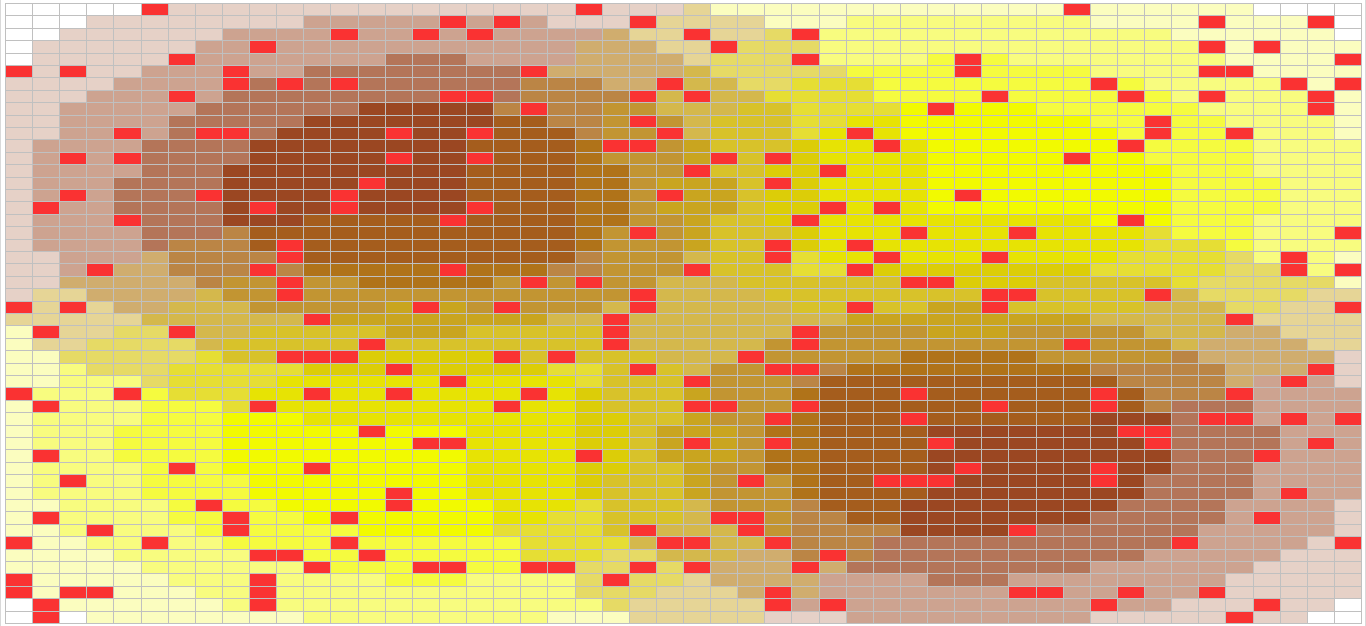
\includegraphics[width=\linewidth]{../../figures/d14.png}
			\\[2pt]
			{\footnotesize (a) Distributed ($d = 14$)}
		\end{minipage}
		\hfill
		\begin{minipage}[t]{0.30\textwidth}
			\centering
			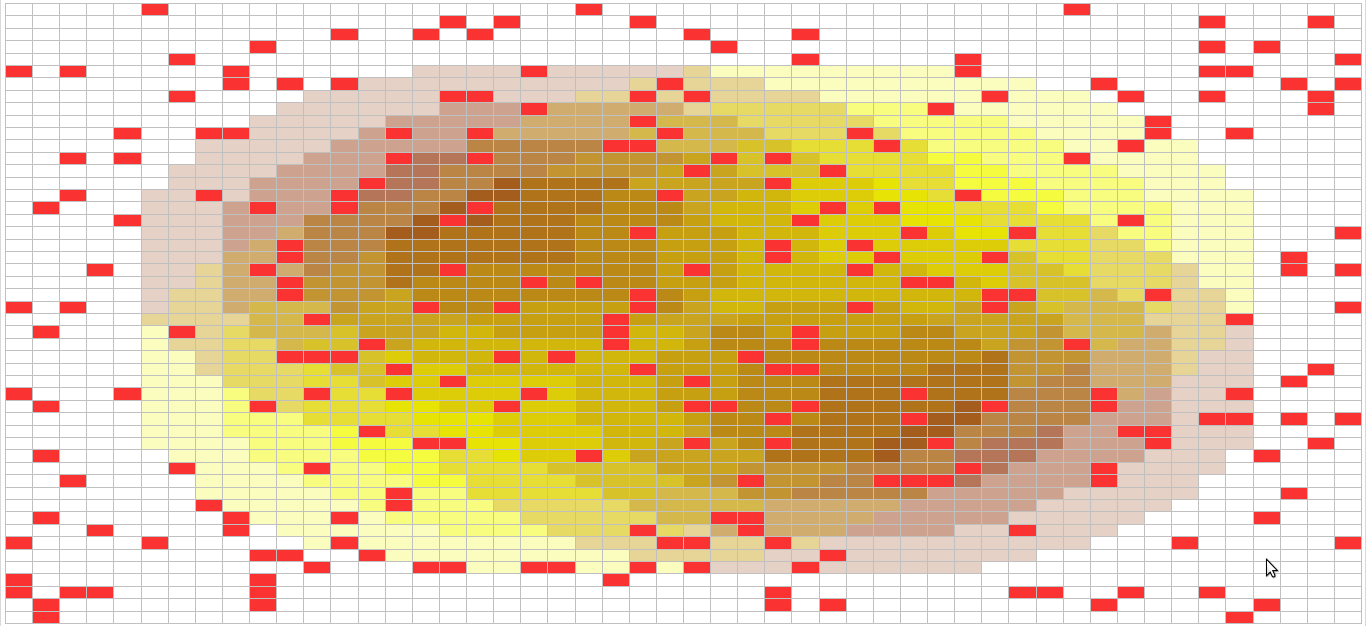
\includegraphics[width=\linewidth]{../../figures/d7.png}
			\\[2pt]
			{\footnotesize (b) Moderately concentrated ($d = 7$)}
		\end{minipage}
		\hfill
		\begin{minipage}[t]{0.30\textwidth}
			\centering
			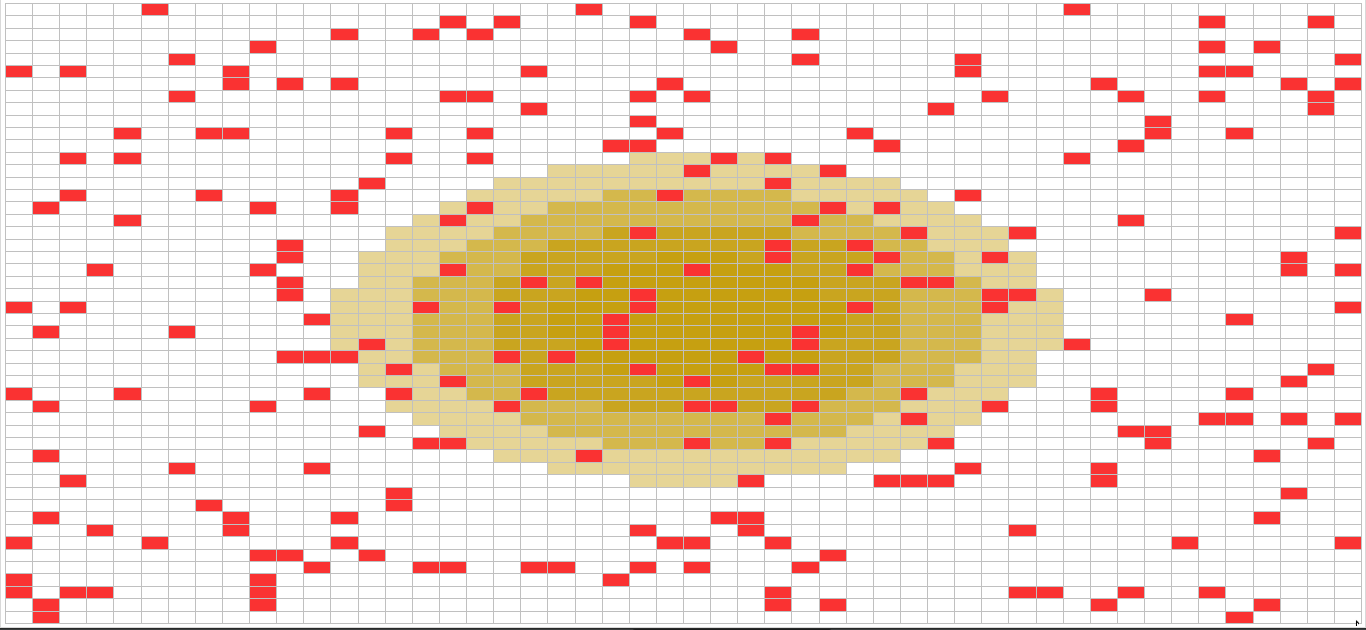
\includegraphics[width=\linewidth]{../../figures/d0.png}
			\\[2pt]
			{\footnotesize (c) Concentrated ($d = 0$)}
		\end{minipage}
		\par\smallskip
		{\footnotesize\noindent\textit{Note.} Each panel shows the 50$\times$50 grid at timestep 0. As $d$ decreases, all four resource peaks converge toward the grid center, reducing spatial diversity of resource access. Yellow represents sugar and brown represents spice. Brighter cells indicate higher resource capacity.}
		\end{figure}

		\newpage
			\subsection{Statement of the Problem}
				\citet{KremerHerman2024} showed that the ethical decision model an agent follows produces different outcomes for the population as a whole. Their experiments, however, were conducted under a single, fixed resource layout. It was not known whether those results were specific to that layout or would hold under different conditions.

				Resource layout directly shapes how agents compete. When resources are spread out, agents can find them in many locations. When resources are concentrated in one spot, all agents compete for the same location, and utilitarian agents are penalized the most because their scoring rule requires them to account for the cost their movement imposes on neighbors. This penalty is largest precisely where competition is most intense.

				It was not known whether the utilitarian advantage would be preserved, reduced, or reversed as resources became more concentrated. It was also not known whether the size of the differences between agent types would stay the same or grow as the resource layout changed. This study addressed these questions by testing all three decision models across three resource layouts and comparing their outcomes at each level.

\newpage
			\subsection{Objectives of the Study}
				The general objective of this study was to examine the effects of resource concentration on the societal outcomes of ethical decision models in the Sugarscape Digital Terrarium simulation. Specifically, this study aimed to:

				\begin{enumerate}
					\item compare the societal outcomes of utilitarian, altruistic, and egoistic decision models across the following resource layouts:
						\begin{itemize}
							\item[a.] distributed ($d = 14$),
							\item[b.] moderately concentrated ($d = 7$), and
							\item[c.] concentrated ($d = 0$);
						\end{itemize}
					\item determine whether the performance advantage of the utilitarian decision model is maintained, strengthened, or weakened as resource peaks converge toward the center;
					\item identify which resource layout produces the most distinct differences in outcomes among the three agent types; and
					\item record and report how long each simulation run took to complete, providing a computational performance benchmark not reported in prior Digital Terrarium experiments.
				\end{enumerate}
\newpage
\subsection{Hypotheses}

Four research questions guided the inferential analysis of this study, formulated around the two inferential study objectives (Objectives~1 and~2). For each question, a formal null hypothesis ($H_0$) and alternative hypothesis ($H_a$) were stated prior to data collection. Study Objectives~3 and~4 were descriptive in nature and required no formal hypothesis test: Objective~3 involved a synthesis interpretation of the effect size results already established under Objective~2, and Objective~4 concerned computational execution time.

\begin{description}

    \item[\textbf{RQ1.}] Do the three ethical decision models produce significantly different societal outcomes under the distributed resource layout ($d = 14$)?

    \smallskip
    \noindent $H_{0,1}$: The utilitarian, altruistic, and egoistic decision models produce no statistically significant differences in final population size, mean agent wealth, societal wealth, Gini coefficient, mean time to live, or extinction rate under the distributed resource layout ($d = 14$).

    \smallskip
    \noindent $H_{a,1}$: At least one ethical decision model produces statistically significantly different societal outcomes from the others under the distributed resource layout ($d = 14$).

    \bigskip
    \item[\textbf{RQ2.}] Do the three ethical decision models produce significantly different societal outcomes under the moderately concentrated resource layout ($d = 7$)?

    \smallskip
    \noindent $H_{0,2}$: The utilitarian, altruistic, and egoistic decision models produce no statistically significant differences in final population size, mean agent wealth, societal wealth, Gini coefficient, mean time to live, or extinction rate under the moderately concentrated resource layout ($d = 7$).

    \smallskip
    \noindent $H_{a,2}$: At least one ethical decision model produces statistically significantly different societal outcomes from the others under the moderately concentrated resource layout ($d = 7$).

    \bigskip
    \item[\textbf{RQ3.}] Do the three ethical decision models produce significantly different societal outcomes under the concentrated resource layout ($d = 0$)?

    \smallskip
    \noindent $H_{0,3}$: The utilitarian, altruistic, and egoistic decision models produce no statistically significant differences in final population size, mean agent wealth, societal wealth, Gini coefficient, mean time to live, or extinction rate under the concentrated resource layout ($d = 0$).

    \smallskip
    \noindent $H_{a,3}$: At least one ethical decision model produces statistically significantly different societal outcomes from the others under the concentrated resource layout ($d = 0$).

    \bigskip
    \item[\textbf{RQ4.}] Does the size of performance differences between ethical decision models vary across the three resource layouts?

    \smallskip
    \noindent $H_{0,4}$: The effect size ($\eta^2_H$, a measure of how large the differences are) of performance differences between ethical decision models does not vary across the three resource layouts ($d = 0$, $d = 7$, $d = 14$).

    \smallskip
    \noindent $H_{a,4}$: The effect size ($\eta^2_H$) of performance differences between ethical decision models varies across at least two of the three resource layouts.

\end{description}

\subsection{Significance of the Study}
Whether the conclusions drawn from ethical agent simulations depend on the resource environment used to generate them is a question with direct implications for how such studies are designed and interpreted. Prior work by \citet{KremerHerman2024} established that utilitarianism outperforms altruism and egoism in agent-based simulation, but that conclusion was drawn from a single, fixed resource environment. By systematically varying resource concentration across three levels, this study tested whether those findings held under environmental pressure, or whether the advantage of a given ethical model depended on conditions that could change. This was a question of practical importance for researchers who use agent-based simulation to draw conclusions about ethical systems: if societal outcomes are sensitive to resource geography, then resource layout is a variable that must be controlled or reported rather than left implicit.

Beyond the scope of Sugarscape research, this study contributed to the broader project of using computational simulation as a tool for ethical inquiry. Agent-based modeling allows researchers to run ethical experiments that would be impractical, harmful, or impossible to conduct with real human populations. By demonstrating that environmental structure interacts with ethical decision-making to determine which orientations survive and which collapse, this study added to the evidence base that resource distribution is not a neutral background condition in ethical agent simulations. The first reported computational benchmark for the Digital Terrarium further supports future replications and parameter sweeps that build on this framework.

\subsection{Scope and Delimitations}
This study was limited to the Sugarscape Digital Terrarium simulation developed by \citet{KremerHerman2024}. All experiments were conducted within this specific implementation, and the findings apply to the behaviors and parameters defined by that framework. Three ethical decision models were examined: utilitarian, altruistic, and egoistic, corresponding exactly to the models provided by the Digital Terrarium. No other ethical frameworks, hybrid models, or agents that can change their decision model during a simulation were introduced or tested.

Resource concentration was defined by a single parameter: $d$, the distance of four resource peaks from the center of the simulation grid. Only three values of $d$ were tested: $d = 14$, $d = 7$, and $d = 0$. $d = 14$ replicated the baseline layout of \citet{KremerHerman2024}; $d = 0$ represented the concentrated extreme where all peaks converge at the grid center; and $d = 7$ was the midpoint ($14 \div 2 = 7$), providing one moderately concentrated measurement between the two extremes. The study did not claim to cover every possible resource layout in Sugarscape or in agent-based modeling generally. Other features of the environment, such as uneven peak placement, varying peak heights, seasonal resource changes, pollution, and disease, were kept at their default values and were not investigated. The simulation grid was fixed at 50 by 50 cells with a starting population of 250 agents, and all other Digital Terrarium settings were kept at their defaults throughout.

Each of the nine experimental conditions was run across 100 independent random seeds, with each run lasting 5000 timesteps. One hundred seeds per condition were chosen based on available computational resources, which is one-fifth of the sample used by \citet{KremerHerman2024}.

Every run used a single decision model for all agents, meaning every agent in a given run was either all-utilitarian, all-altruistic, or all-egoistic. Populations that mix different decision models were not tested. Agent-level data such as individual resource collection records and per-agent wealth over time were not logged or analyzed. The study did not make claims about real human ethical behavior, real-world policy outcomes, or the moral value of any ethical theory. Its conclusions apply only to the behavior of agents operating under the specific decision rules of the Digital Terrarium within the three tested resource layouts.

		
\section{REVIEW OF LITERATURE}
\subsection{Ethical Decision-making}
Ethical decision-making refers to the process of assessing and selecting among possible actions in a manner that is consistent with accepted ethical principles \citep{Pembi2024}. It is the cognitive and behavioral process used to explain and navigate complex, ambiguous, and high-stakes ethical dilemmas. It has been used by  organizations and scholars to provide frameworks for ethical conduct and its large-scale implications \citep{MacDougall2014}. 

The significance of ethical decision-making  is evident when faced with real-world dilemmas spanning across medical, economic and administrative fields. Public sectors in Turkey had been doing unethical activities that challenged professional values including bribery and extortion; it moved from individual level to institutional which is characterized as an “intensive and common ethical depression” \citep{CigerogluOztepe2019}.  In machine learning, there is a risk that “principle learning” could result in internal development of immoral principles by the agent, especially if the reasoning process is a “black box” \citep{Miranda2010}.  A self-driving car mirrors the trolley problem if it were forced to choose between the safety of its passengers and the lives of bystanders in an unavoidable accident \citep{KremerHerman2024}. Widespread integration of AI tools into content creation introduced a new frontier of plagiarism which erodes the foundation of original thought and intellectual honesty \citep{Joshi2025}. 

There are several ethical models and theories that serve as a framework to help people distinguish between ethical and unethical decisions. \citet{Whittier2006} identified three types of models: normative, descriptive, and prescriptive models. \citet{Pembi2024} defined four main theories: rights, justice, caring, and utilitarian theories.

\newpage
\citet{Whittier2006} built a set of criteria to evaluate ethical decision-making models' adequacy. In the process of building this, they had found three types of models that dominated their literature: normative, prescriptive, and descriptive models. Normative models specify how choices should ideally be made. Prescriptive models aim to improve choices under real-world constraints. Descriptive models consider empirical evidence to explain how choices are actually made. From these three models, the study leaned toward making the agent's decision-making a descriptive model.

\citet{Pembi2024} analyzed theoretical frameworks to help managers in corporate decision-making. They defined four main theories: rights, justice, caring, and utilitarian theories. Rights theory states that ethical decision-making is the most effective way to protect and uphold the fundamental rights and privileges of all individuals affected.  Justice theory addresses issues of abuse and unfair treatment particularly within organizations. Caring theory emphasizes the importance of relationships and interdependence in moral life; it is developed largely through feminist ethical thought. Utilitarian theory works in this central principle: to achieve “the greatest good for the greatest number" (\citealt{WhiteTaft2004}, as cited in \citealt{Pembi2024}). These ethical theories collectively provide the conceptual foundation for the study. However, the primary theory the study used was utilitarianism due to its quantitative nature. 

\subsection{Bentham's Felicific Calculus}
Utilitarianism is rooted in the pragmatic ideas of Jeremy Bentham and John Stuart Mill in the 18th and 19th centuries. It is based on the assumption that knowledge and decisions should be grounded in observable, objective, and verifiable data. It prioritizes overall welfare over considerations such as rights, duties, or justice. In evaluating ethical choices, this theory adopts a societal perspective, assessing actions based on their overall consequences in terms of the balance between good and harm (\citealt{WhiteTaft2004}, as cited in \citealt{Pembi2024}).

Bentham's felicific calculus is a morality system produced by the Utilitarianism movement that compares the pain and pleasure an action has created \citep{Majot2014}. It is a deliberation method or technical tool used to operationalize the principle of utility \citep{Baujard2009}. 

The principle of utility, also called the greatest happiness principle, is the foundational ethical standard that defines how right or wrong an action is based on its tendency to increase or decrease the happiness of the party involved \citep{Bentham1907,Baujard2009}. According to this principle, pain and pleasure shape people's understanding of right and wrong and influence every action, thought, and decision they make even if individuals claim to reject this influence. This principle is based on the recognition that people naturally seek outcomes that maximize happiness or felicity. This principle was proposed by Bentham to be the basis for moral reasoning and legal systems rather than relying on abstract rhetoric or metaphor (\citealt{Bentham1789}, as cited in \citealt{Baujard2009}). 

To quantify pleasure and pain, the seven dimensions of utility were identified by \citet{Bentham1907}. These are intensity, duration, certainty, propinquity, fecundity, purity, and extent. Table~\ref{table:felicific-criteria} summarizes each dimension and its scope of application.

		\begin{table}[H]
		\vspace{2ex}
		\centering
		\caption{Bentham's Seven Dimensions of Utility in the Felicific Calculus}
		\label{table:felicific-criteria}
		\footnotesize
		\renewcommand{\arraystretch}{1.3}
		\begin{tabular}{
			>{\raggedright\arraybackslash}p{2.4cm}
			>{\raggedright\arraybackslash}p{10.0cm}
		}
		\hline\hline
		\textbf{Criterion} & \textbf{Description} \\
		\hline
		Intensity    & The strength or vividness of the pleasure or pain experienced \\
		Duration     & How long the pleasure or pain lasts \\
		Certainty    & The probability that the pleasure or pain will actually occur \\
		Propinquity  & How near in time the pleasure or pain is to the present moment \\
		\hline
		Fecundity    & Likelihood that similar sensations will follow the experience \\
		Purity       & Likelihood that opposite sensations will \textit{not} follow the experience \\
		\hline
		Extent       & Number of individuals affected by the action \\
		\hline
		\end{tabular}
		\par\smallskip

		\end{table}

When estimating pain or pleasure by itself, four of these dimensions are considered: intensity, duration, certainty, and propinquity. Intensity is how pleasant the pleasure or pain is. Duration is how long the pleasure or pain would last. Certainty is the probability that the pleasure or pain will occur. Propinquity is how near in time the pleasure or pain is.

When evaluating the consequences of an action, two additional factors should also be considered: fecundity and purity. Fecundity is the likelihood that the experience will be followed by similar sensations, and purity is the likelihood that it will not be followed by the opposite sensation. However, these two factors are not direct qualities of the pleasure or pain itself, but rather characteristics of the action that produces them. When considering the effects of pleasure or pain on a group of people, another factor must be added: extent, which refers to the number of individuals affected by the action  \citep{Bentham1907,Sprigge1999}.

Bentham's felicific calculus bridges two ideas: moral welfarism, the ethical goal of maximizing welfare or happiness, and technical non-welfarism, the practical use of proxy variables when welfare cannot be directly measured \citep{Baujard2006}. The felicific calculus is inordinately tedious, expensive, and often impossible to implement in the real world because accurately measuring individual utility is not always possible \citep{Baujard2006}. Although moral welfarism assumes that individual utility is the only relevant consideration, practitioners cannot directly observe a person's internal thoughts or preferences \citep{Baujard2006}. By knowing how to move toward technical non-welfarism, practical proxies have been used by decision makers to estimate utility in ways that are more feasible for public policy \citep{Baujard2006}. 

Proxies are external, observable indicators that serve as substitutes for unobservable internal states like utility or happiness. They have been used  to perform practical calculations since utility is a theoretical construct with no objective measurement unit \citep{Li2002}.

There are different types of proxies used across different fields. Money has been suggested as a “measuring rod” by Bentham since it does not require a lot of information and its amount reflects how much people value or prefer something \citep{Baujard2006}. Secondary circumstances such as sex, age, rank, education, and religious profession were also suggested by Bentham since these “very visible traits” are not the definition of utility itself but are highly correlated with an individual's "bias of sensibility," making them reliable proxies for legal and judicial decisions \citep{Baujard2009}. Indexes and scoreboards such as Human Development Index (HDI) summarize complex, interdependent phenomena that are not directly observable \citep{Munda2020}. In digital simulations, specifically in Sugarscape, the consumption of sugar and spice acts as a proxy for happiness  \citep{KremerHerman2024}. In this study, this use of proxy to estimate utility was evident in the Digital Terrarium simulation. 

In the Digital Terrarium simulation, agents must continuously evaluate possible actions based on local state conditions, resource availability, and interactions with other agents. This makes agent-based modeling a suitable framework for operationalizing Bentham's felicific calculus, as the dimensions of utility can be translated into quantifiable indicators for decision-making.

\subsection{Agent-based Modeling}
Agent-based modeling is a computational method in computer simulations designed to examine how processes at the micro level influence outcomes at the macro level \citep{Scalco2015}. This is a “bottom-up approach” where the simulation models individual agents and allows system behaviour to emerge from their interactions \citep{Kehoe2015}. This modeling paradigm was advanced by artificial societies with human and social factors integrated to the model  \citep{Tolk2022}.

\citet{Tolk2022} identified the three primary elements of artificial societies: individual agents, social networks, and situated environment.
Individual agents are entities that form the building blocks of an artificial society. They are autonomous units that interact at the micro-level based on their own rules \citep{KremerHerman2024}. They are heterogeneous units with different information, backgrounds, and decision-making rules \citep{Lempert2002}. They follow a “perceive-and-act” cycle governed by their inner logic, typically through probability rules or conditional statements \citep{Tolk2022}.

Social networks capture various affiliations, interactions, and embedded structures that influence how individuals behave and how policies impact the population. They represent the diverse social groups to which an agent belongs, which dictate the behaviour it needs to select  \citep{Tolk2022}.  They are viewed as networks of intelligent adaptive agents that affect macro-level performance of an organization (Carley, 2002, as cited in \citealt{Lempert2002}). In Sugarscape, these social networks are often represented as tribes; it is a group of agents sharing the same “cultural tags” \citep{KremerHerman2024}.

Situated environment provides the infrastructure and social drivers that shape agent behaviours and policy outcomes. It is the surrounding situation being perceived by the agent when they act with their inner logic \citep{Tolk2022}. It is a digital landscape that enables the simulation of resource scarcity or abundance and how it affects the artificial society \citep{KremerHerman2024}.

This study used these three elements to model agent decision-making as a dynamic process in which agents compare possible actions through felicific vectors and select the option that most closely aligns with their preferred outcomes within a given social and environmental context. To operationalize this, the study adopted the Digital Terrarium simulation by \citet{KremerHerman2024} implemented through the Sugarscape model.

\subsection{Sugarscape Model}
Sugarscape is the first large-scale agent-based social simulation developed and presented by \citet{EpsteinAxtell1996} in their  book “Growing Artificial Societies”. It is frequently used as a benchmark for agent-based modeling toolkits such as Swarm, Repast, and Netlogo. It was used to explore how different social networks can be influenced by individual decisions within the population \citep{Kehoe2015}. Its mechanism can be divided into three parts: environment, agents, and interactions.

\subsubsection{Sugarscape Environment}	
The Sugarscape environment provides the physical space upon which agents interact. It is structured as a discrete two-dimensional M by M toroidal grid; it wraps around all four edges where an agent, for instance, can move to the left edge and reappear on the right edge. Each grid cell can only hold one agent at a time. For the agents' interaction space, the simulation uses the von Neumann neighborhood; it is the adjacent cells to the left, right, top, and down of a grid cell \citep{Kehoe2015}. 

Its environment has specifications for resource dynamics. There are two main resources in this model: sugar and spice, where spice is a second resource introduced to enable trading. Each resource has a fixed maximum limit for each grid cell called the carrying capacity. These resources are not permanent as they regenerate at a predefined rate up to the grid cell's carrying capacity \citep{Kehoe2015}. 

This physical space is not static and can undergo large-scale changes over time called seasons. Its grid is divided into two parts: the top half is summer and the bottom half is winter. Resources grow back at full rate during summer, and they grow back at a significantly slower rate during winter. This feature is toggleable, including the seasonal regrowth rules \citep{Kehoe2015}. 

The environment simulates side-effects for gathering and consuming resources called pollution. This pollution spreads across the space where the pollution level at each site is updated to the average of its von Neumann neighbors; this spread of pollution is called pollution diffusion. When a location is polluted, a new location would be chosen by an agent based on a welfare function that considers the resource-to-pollution ratio \citep{Kehoe2015}. 
\subsubsection{Sugarscape Agents}	
The Sugarscape agents are defined by internal traits that determine their physical and survival needs: metabolism, vision, age, and resource store. Metabolism is the rate at which an agent consumes sugar and spice every turn; once the agent's resource store is depleted, the agent dies. Vision determines how many grid cells an agent can see to find resources or other agents. Age is how long the agent is present in the simulation. Resource store is the amount of sugar and spice the agent has in the beginning of the simulation  \citep{Kehoe2015}.

These agents are not identical as they carry the following traits that define their place in the artificial society: sex, fertility, cultural tag, disease, and immunity. Sex assigned to an agent is either male or female. Fertility is the age-dependent property that enables an agent to mate with others. Cultural tag is the bit sequence the agent carries that defines its cultural identity or tribe. Disease is a bit sequence that increases the metabolism of an agent by one unit; an agent can carry at least one disease and can be passed between agents. Immunity is a bit sequence that can protect against certain diseases \citep{Kehoe2015}.

\subsubsection{Sugarscape Interactions}	
The Sugarscape interactions are local rules designed to model a wide array of social, economic, and biological phenomena. Local-level interactions are restricted by an agent's vision; these include movement, mating, trading, lending, cultural transmission, disease transmission, and aggression. For movement, agents search their visible neighborhood for unoccupied sites and move to the nearest location with the highest welfare. For mating, it occurs when two adjacent agents are of opposite sexes, both are fertile, and at least one empty neighboring site is available for the offspring. For trading, agents with different marginal rates of substitution exchange sugar and spice until no further mutually beneficial trade is possible. For lending, neighboring agents borrow and lend resources to each other. For cultural transmission, also called tagging, agents may spread culture tags to others. For disease transmission, agents may also spread disease to their neighbors. For aggression, it occurs through combat where agents may attack weaker members of another tribe and seize their resources \citep{Kehoe2015}.

The Sugarscape model demonstrates how complex social, economic, and biological phenomena can emerge from relatively simple rule-based interactions among agents within a structured environment. This model was extended by \citet{KremerHerman2024} into what they called the ``Digital Terrarium,'' which further refined the operationalization of ethical decision-making under Bentham's felicific calculus.

\subsubsection{Digital Terrarium}
The Digital Terrarium is an extension of the Sugarscape agent-based model developed by \citet{KremerHerman2024}. It replaces the greedy movement rule of standard Sugarscape with a felicific calculus-based decision procedure that operationalizes Bentham's dimensions of utility into computable welfare scores. Each timestep, every agent selects a destination cell by scoring all reachable candidates and moving to the one with the highest aggregated welfare score. Social interactions, including combat, reproduction, trade, and lending, are not separately decided; they trigger automatically as mechanical consequences of the selected cell. Figure~\ref{fig:digital-terrarium} shows a representative state of the simulation environment at a single timestep.

		\begin{figure}[H]
		\centering
		\caption{The Sugarscape Digital Terrarium simulation environment}
		\label{fig:digital-terrarium}
		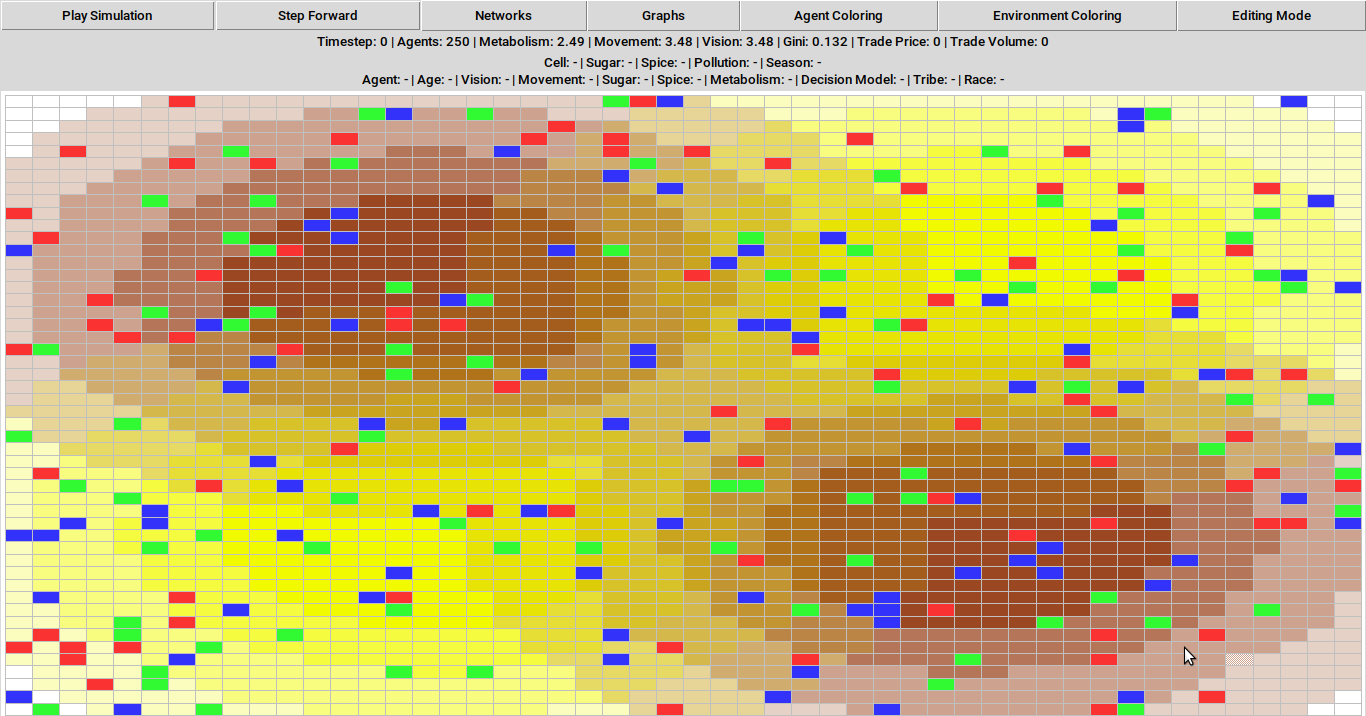
\includegraphics[width=0.6\linewidth]{../../figures/digital-terrarium.png}
		\end{figure}

The grid encodes two types of resources through color: yellow cells contain sugar and brown cells contain spice, with color saturation indicating resource abundance, where a more saturated cell holds a greater quantity of that resource. Three agent types are distinguished by color: green agents are altruistic ($\phi = 0.0$), red agents are egoistic ($\phi = 1.0$), and blue agents are utilitarian ($\phi = 0.5$). At each timestep, agents scan the cells within their range, score each candidate using the felicific calculus, and move toward the highest-scoring cell. As agents converge on resource-rich regions, social interactions (including combat, reproduction, trade, and lending) are triggered automatically based on which agents share or contest the same cell. The resulting population dynamics emerge from the accumulated effect of these individual decisions across thousands of timesteps, without any centralized coordination.

The mechanics underlying each agent's decision at every timestep consist of three steps: candidate enumeration, per-person welfare computation, and cell selection.

\textbf{Candidate Enumeration.}
The set of candidate cells available to an agent is bounded by its effective range \citep{KremerHerman2024}:
\begin{equation}
	\text{cellRange} = \min(\text{vision},\ \text{movement})
\end{equation}
\begin{figure}[H]
\caption{Computing the effective cell range for candidate enumeration.}
\begin{lstlisting}[language=Python, firstnumber=770]
cellRange = min(min(vision, movement),
                self.cell.environment.maxCellDistance)
\end{lstlisting}
{\footnotesize\noindent\textit{Note.} From \citet{KremerHerman2024}. \texttt{agent.py}, \texttt{Agent.findCellsInRange} (line~770).}
\end{figure}
In cardinal movement mode, only cells sharing the agent's row or column qualify, up to $\text{cellRange}$ steps in each of the four cardinal directions. The agent's current cell is always retained as a fallback candidate.

\textbf{Per-Person Welfare Components.}
For each candidate cell $c$, the agent computes a welfare score for itself and for every neighbor that can also reach $c$. Let $k$ denote any agent (self or neighbor) capable of reaching $c$, $W_c$ the total resources at cell $c$, $W_{c,\mathrm{max}}$ the cell's maximum resource capacity, $m_k$ agent $k$'s combined metabolic rate (sugar metabolism plus spice metabolism), $\text{TTL}_k$ the number of timesteps agent $k$ can survive on its current resource store, and $|V|$ the total number of cells within the agent's range.

The immediate social density weight $e$ is the ratio of live neighbors visible from the agent's current position to the total cells in range \citep{KremerHerman2024}:
\begin{equation}
	e = \frac{|\text{neighbors visible from current cell}|}{|V|}
\end{equation}
\begin{figure}[H]
\caption{Computing the immediate social density weight \(e\).}
\begin{lstlisting}[language=Python, firstnumber=180]
cellsInRange = len(neighbor.cellsInRange)
extent = neighborhoodSize / cellsInRange if cellsInRange > 0 else 1
\end{lstlisting}
{\footnotesize\noindent\textit{Note.} From \citet{KremerHerman2024}. \texttt{ethics.py}, \texttt{Bentham.findEthicalValueOfCell} (lines~180--181).}
\end{figure}

The immediate intensity $i_k$ operationalizes Bentham's intensity and certainty dimensions, increasing as an agent's time-to-live decreases or cell pollution rises \citep{KremerHerman2024}:
\begin{equation}
	i_k = \frac{1}{(1 + \text{TTL}_k)(1 + \text{pollution})}
\end{equation}
\begin{figure}[H]
\caption{Computing the immediate intensity \(i_k\).}
\begin{lstlisting}[language=Python, firstnumber=170]
intensity = (1 / (1 + neighbor.findTimeToLive())
             / (1 + cell.pollution))
\end{lstlisting}
{\footnotesize\noindent\textit{Note.} From \citet{KremerHerman2024}. \texttt{ethics.py}, \texttt{Bentham.findEthicalValueOfCell} (line~170).}
\end{figure}

The immediate duration $d_k$ operationalizes Bentham's duration dimension, reflecting how long the candidate cell's resources would sustain agent $k$ relative to the cell's maximum capacity \citep{KremerHerman2024}:
\begin{equation}
	d_k = \frac{W_c / m_k}{W_{c,\mathrm{max}}}
\end{equation}
\begin{figure}[H]
\caption{Computing the immediate duration \(d_k\).}
\begin{lstlisting}[language=Python, firstnumber=168]
cellDuration = (cellSiteWealth / neighborMetabolism
                if neighborMetabolism > 0 else 0)
duration = (cellDuration / cellMaxSiteWealth
            if cellMaxSiteWealth > 0 else 0)
\end{lstlisting}
{\footnotesize\noindent\textit{Note.} From \citet{KremerHerman2024}. \texttt{ethics.py}, \texttt{Bentham.findEthicalValueOfCell} (lines~168--171).}
\end{figure}

The future social density weight $e_f$ is recomputed per candidate cell using neighbors visible from the candidate position rather than the current position \citep{KremerHerman2024}:
\begin{equation}
	e_f = \frac{|\text{neighbors visible from candidate cell } c|}{|V|}
\end{equation}
\begin{figure}[H]
\caption{Computing the future social density weight \(e_f\).}
\begin{lstlisting}[language=Python, firstnumber=182]
futureExtent = (futureNeighborhoodSize / cellsInRange
                if cellsInRange > 0
                and self.decisionModelLookaheadFactor != 0
                else 1)
\end{lstlisting}
{\footnotesize\noindent\textit{Note.} From \citet{KremerHerman2024}. \texttt{ethics.py}, \texttt{Bentham.findEthicalValueOfCell} (line~182).}
\end{figure}

The future intensity $i_f$ reflects the resource richness of the candidate cell's immediate neighborhood, where $W_{\text{adj}}$ is the summed wealth of all adjacent cells, $W_{g,\mathrm{max}}$ is the global maximum possible wealth in the environment, and $n_{\text{adj}}$ is the number of adjacent cells \citep{KremerHerman2024}:
\begin{equation}
	i_f = \frac{W_{\text{adj}}}{W_{g,\mathrm{max}} \times n_{\text{adj}}}
\end{equation}
\begin{figure}[H]
\caption{Computing the future intensity \(i_f\).}
\begin{lstlisting}[language=Python, firstnumber=177]
cellNeighbors = len(neighbor.cell.neighbors)
futureIntensity = (cellNeighborWealth
                   / (globalMaxWealth * cellNeighbors))
\end{lstlisting}
{\footnotesize\noindent\textit{Note.} From \citet{KremerHerman2024}. \texttt{ethics.py}, \texttt{Bentham.findEthicalValueOfCell} (lines~177--178).}
\end{figure}

The future duration $d_{f,k}$ is the residual resources remaining at $c$ after agent $k$ consumes one timestep's worth of metabolism \citep{KremerHerman2024}:
\begin{equation}
	d_{f,k} = \frac{W_c - m_k}{m_k \times W_{c,\mathrm{max}}}
\end{equation}
\begin{figure}[H]
\caption{Computing the future duration \(d_{f,k}\).}
\begin{lstlisting}[language=Python, firstnumber=174]
futureDuration = ((cellSiteWealth - neighborMetabolism)
                  / neighborMetabolism
                  if neighborMetabolism > 0
                  else cellSiteWealth)
futureDuration = (futureDuration / cellMaxSiteWealth
                  if cellMaxSiteWealth > 0 else 0)
\end{lstlisting}
{\footnotesize\noindent\textit{Note.} From \citet{KremerHerman2024}. \texttt{ethics.py}, \texttt{Bentham.findEthicalValueOfCell} (lines~174--175).}
\end{figure}

\textbf{Per-Person Welfare Score.}
The individual welfare score $h_k$ for agent $k$ evaluating candidate cell $c$ aggregates the immediate and future welfare components, weighted by social density and discounted by a temporal factor $\gamma \in [0, 1]$ \citep{KremerHerman2024}:
\begin{equation}
	h_k = (c_k \times p) \left[ e(i_k + d_k) + \gamma\, e_f(i_f + d_{f,k}) \right]
\end{equation}
where $c_k \in \{0,1\}$ indicates whether agent $k$ can reach cell $c$, and $p = 1$ (propinquity, fixed at one-step lookahead). The term $e(i_k + d_k)$ captures immediate welfare weighted by social density, while $\gamma\, e_f(i_f + d_{f,k})$ captures discounted future welfare. This formulation is structurally equivalent to the Bellman optimality equation of a Markov Decision Process \citep{KremerHerman2024}:
\begin{equation}
	V^*(s) = \max_a \sum_{s'} T(s, a, s')\left[ R(s, a, s') + \gamma V^*(s') \right]
\end{equation}
where $T(s, a, s')$ maps to $c_k \times p$, $R(s, a, s')$ maps to $e(i_k + d_k)$, and $\gamma V^*(s')$ maps to $\gamma\, e_f(i_f + d_{f,k})$.
\begin{figure}[H]
\caption{Computing the per-person welfare score \(h_k\).}
\begin{lstlisting}[language=Python, firstnumber=185]
currentReward = extent * (intensity + duration)
futureReward = futureExtent * (futureIntensity
                               + futureDuration)
neighborCellValue = ((certainty * proximity)
                     * (currentReward
                        + (discount * futureReward)))
\end{lstlisting}
{\footnotesize\noindent\textit{Note.} From \citet{KremerHerman2024}. \texttt{ethics.py}, \texttt{Bentham.findEthicalValueOfCell} (lines~185--187).}
\end{figure}

\textbf{Ethical Aggregation via the Selfishness Factor.}
After computing $h_k$ for every agent that can reach $c$, the candidate cell's final score $h(c)$ is determined by the selfishness factor $\phi \in [0, 1]$ \citep{KremerHerman2024}:
\begin{equation}
	h(c) = \phi\, h_{\text{self}} - (1 - \phi) \sum_{k \neq \text{self}} h_k
\end{equation}
\begin{figure}[H]
\caption{Aggregating welfare scores using the selfishness factor \(\phi\).}
\begin{lstlisting}[language=Python, firstnumber=190]
if neighbor != self and self.selfishnessFactor < 1:
    neighborCellValue = -1 * neighborCellValue
# ...
if neighbor == self:
    neighborCellValue *= self.selfishnessFactor
else:
    neighborCellValue *= 1 - self.selfishnessFactor
cellValue += neighborCellValue
\end{lstlisting}
{\footnotesize\noindent\textit{Note.} From \citet{KremerHerman2024}. \texttt{ethics.py}, \texttt{Bentham.findEthicalValueOfCell} (lines~190--234).}
\end{figure}
The selfishness factor encodes the agent's ethical orientation. An egoistic agent sets $\phi = 1.0$, giving full weight to self-gain and ignoring neighbor welfare entirely. A utilitarian agent sets $\phi = 0.5$, weighting self-gain and collective harm equally. An altruistic agent sets $\phi = 0.0$, excluding own welfare entirely and selecting the cell that minimizes summed harm to neighbors. The standard Sugarscape agent bypasses this formula, scoring each cell as the raw sum of its sugar and spice.

\textbf{Cell Selection.}
The welfare component computation, welfare score aggregation, and ethical weighting described above are applied independently to every candidate cell. The agent then selects the cell with the highest aggregate score \citep{KremerHerman2024}:
\begin{equation}
	c^* = \arg\max_{c}\ h(c)
\end{equation}
\begin{figure}[H]
\caption{Selecting the optimal candidate cell by ethical score \(c^*\).}
\begin{lstlisting}[language=Python, firstnumber=113]
for cell in cells:
    cell["wealth"] = self.findEthicalValueOfCell(cell["cell"])
if self.selfishnessFactor >= 0:
    for cell in cells:
        if cell["wealth"] > 0:
            bestCell = cell["cell"]
            break
\end{lstlisting}
{\footnotesize\noindent\textit{Note.} From \citet{KremerHerman2024}. \texttt{ethics.py}, \texttt{Bentham.findBestEthicalCell} (lines~113--119).}
\end{figure}
When two cells share the highest score, the closer one is preferred. The agent moves directly to $c^*$ in a single step, and any social interactions enabled by the new position are resolved automatically by the environment.

\subsection{Related Studies}
Direct experimentation on human societies to test ethical systems is neither practical nor ethically acceptable. Because of this, agent-based simulation provides a useful way to study how different moral decision-making rules affect collective social outcomes. In these simulations, agents do not act independently of their environment. The distribution of resources influences whether societies remain stable or collapse, how wealth is shared or concentrated, and which behaviors increase an agent's chances of survival. When resources become highly concentrated in specific areas, the environment creates pressure that can increase inequality, intensify competition, and threaten population stability. However, societal outcomes are shaped not only by environmental conditions but also by the ethical composition of the population. The proportion and interaction of different ethical agents may determine whether societies adapt successfully to environmental pressure or move toward instability. Therefore, there is a need to investigate whether the societal outcomes produced by ethical decision-making models under balanced resource conditions remain consistent as resource distributions become progressively more extreme.

\subsubsection{Ethical Experimentation Through Agent-Based Simulation}
Conducting ethical and policy experiments in the real world often carries prohibitive risks and moral costs because social systems can react unpredictably to changes in resource distribution and behavioral rules. Agent-based simulation provides a controlled alternative where ethical theories can be tested in virtual environments without the real-world consequences of actual policy intervention \citep{Tolk2022}.

\citet{KremerHerman2024} tested three ethical decision models in a Sugarscape-based digital terrarium: utilitarian agents that weigh their own welfare equally with their neighbors', altruistic agents that prioritize only neighbor welfare, and egoistic agents that act purely in self-interest. Across all experimental conditions, utilitarian societies consistently achieved the largest populations, the longest survival periods, and the greatest accumulated societal wealth. Egoist societies experienced what the authors call a "murderous period" in which agents competed violently over resources, leaving behind only a few wealthy survivors isolated in resource-rich enclaves \citep{KremerHerman2024}. Altruist societies failed for the opposite reason: agents that excluded their own welfare from decision-making engaged in rampant self-sacrifice, depleting their own resources to benefit neighbors and eventually collapsing the population \citep{KremerHerman2024}. \citet{Xiang2008} observed a parallel dynamic in an evolutionary game framework. Altruistic agents, who absorbed individual costs to benefit others, compensated for their disadvantage by clustering spatially, creating local environments where cooperative payoffs stabilized collective outcomes. Selfish agents performed well individually but introduced volatile dynamics at the population level. Both agent-type populations fluctuated sharply at the outset before eventually reaching a new equilibrium, suggesting that mixed-ethics populations pass through an unstable transitional phase before settling \citep{Xiang2008}. At the system level, \citet{Scalco2015} found that altruist-dominated societies generated higher average wealth than egoist-dominated ones in an Ultimatum Game simulation, even though individual altruists made costlier offers. These findings collectively support agent-based simulation as a productive framework for studying ethical outcomes: individual-level ethical rules produce measurable, replicable differences in collective societal performance.

\subsubsection{Operationalizing Ethics in Computational Agents}
Translating abstract philosophical ethics into executable code is a central challenge in agent-based modeling. To build valid ethical agents, researchers must convert subjective human values into measurable, algorithmic inputs that machines can process.

\citet{Majot2014} proposed that running a utilitarian felicific calculus computationally requires a form of synthetic empathy: the agent must estimate the internal states of those around it using observable proxies such as location, current activity, and age. Because no agent can access the true experience of its neighbors, it must perform real-time abstraction of their condition, constructing an approximation of their pain or pleasure from visible behavioral signals. This approach is consistent with \citeauthor{Baujard2009}'s (\citeyear{Baujard2009}) concept of technical non-welfarism: since direct measurement of utility is impossible, agents must use observable proxy variables as practical substitutes. In Sugarscape, the amount of sugar and spice an agent holds serves as the primary proxy for happiness, providing a quantifiable stand-in for the dimensions of utility that Bentham's felicific calculus identifies \citep{KremerHerman2024}.

The Digital Terrarium makes this operationalization explicit through a selfishness factor $\phi \in [0, 1]$ that encodes each agent's ethical orientation. An egoist sets $\phi = 1.0$, maximizing self-gain while ignoring neighbor welfare entirely; a Bentham utilitarian sets $\phi = 0.5$, weighting self-gain and collective harm equally; an altruist sets $\phi = 0.0$, selecting the cell that minimizes summed harm to neighbors while excluding its own welfare from the score \citep{KremerHerman2024}. This single parameter provides a continuous, mathematically grounded bridge between abstract ethical theory and computable agent behavior, enabling systematic comparison of ethical models across varying environmental conditions.

\subsubsection{Resource Distribution and Spatial Dynamics in Artificial Societies}
The spatial distribution of resources within an environment is a highly meaningful and measurable variable that dictates both the success of individual agents and the overarching stability of a population. Altering the geographic topology of resources, whether through macro-level distributions or micro-level gradients, fundamentally changes how societies evolve, how wealth is distributed, and which movement strategies are most effective.

\citet{Hawick2014} demonstrated this directly by comparing two resource configurations in Sugarscape: a twin-peak layout, where sugar was concentrated at two opposing corners of the grid, and a flat layout, where resources were distributed uniformly across all cells. Under the flat configuration, resource access was equal for all agents regardless of starting position, and most individuals maintained similar levels of wealth throughout the simulation. Under the twin-peak configuration, agents near the peaks accumulated far more wealth than those on the surrounding plains, producing a highly unequal distribution. The topology of the resource map directly determined whether a roughly equal ``middle class'' formed or whether extreme wealth disparity took over almost immediately \citep{Hawick2014}.

The significance of resource distribution extends beyond its direct effect on wealth accumulation. \citet{Fagan2022} examined six movement-switching strategies in dynamically shifting patch landscapes and found that the type of information a consumer uses to guide movement is as important as the movement itself. Agents that tracked spatial and temporal gradients, meaning the rate at which resource availability changed over space and time, consistently achieved higher resource-matching success than agents that tracked raw resource density or followed the positions of neighboring consumers. This finding suggests that the informational demands of successful resource acquisition change with the structure of the environment.

\subsubsection{Concentrated Resource Pressure and Societal Inequality}
When resources are not distributed evenly but instead concentrated in specific geographic zones, the resulting environmental pressure fundamentally alters the social and competitive dynamics of an artificial society. This spatial concentration breeds intense competition, extreme inequality, and high-stakes survival strategies that can drive populations toward either adaptation or complete extinction.

\citet{Hawick2014} quantified this trade-off directly. In the flat resource configuration, all agents consumed the environment at a roughly equal rate, depleting it in approximately 300 steps before the entire population starved. In the twin-peak configuration, agents on the resource-poor plains died early from starvation, reducing the population sharply. However, the agents that survived near the peaks sustained themselves for approximately 600 steps, twice as long as in the flat case \citep{Hawick2014}. Geographic concentration therefore extended system longevity at the cost of early mass mortality and extreme wealth inequality.

The interaction between movement range and peak concentration produced a further non-obvious result. When agents could move over large distances in the twin-peak layout, the Gini coefficient of wealth stabilized near 0.5 for much of the simulation. However, greater movement range also caused the system to crash earlier under concentrated conditions, because the sugar remnants after peak erosion were locally clustered. Agents that moved too far from the eroding peaks lost access to the only remaining resources \citep{Hawick2014}. This indicates that under concentrated resource conditions, mobility becomes a double-edged variable: it increases competitive reach but also increases the risk of straying from viable resource remnants.

\citet{Fagan2022} provide a complementary finding from a theoretical ecology perspective. In single-patch landscapes, the closest analog to a maximally concentrated resource environment, resource-matching success was lower and more variable than in two-patch landscapes, because locating and efficiently exploiting a single concentrated source placed higher navigational demands on consumers. As the number of resource patches decreases, consumers must find fewer targets more precisely, raising the cost of any navigational error.

\subsubsection{Ethical Population Composition and System Stability}
In societies where agents operate under different moral frameworks, the ethical composition of the population interacts heavily with environmental pressures to determine the system's stability. By varying the proportions of selfish, altruistic, and utilitarian agents, researchers can identify distinct mathematical tipping points where societies either stabilize and thrive or collapse into extinction.

\citet{KremerHerman2024} systematically varied the selfishness factor of simulated populations from fully altruistic to fully egoistic. Societies operating between 5\% and 85\% selfishness achieved outcomes comparable to a perfectly balanced utilitarian society, indicating a wide zone of viable ethical compositions. Outside this range, instability emerged sharply at both extremes: purely altruistic societies collapsed through self-sacrifice, while societies exceeding 85\% selfishness became highly volatile, with up to one-fifth of all agents dying each timestep \citep{KremerHerman2024}. Notably, introducing even a minimal degree of self-interest, as little as 1\%, was sufficient to prevent the collapse of a purely altruistic society, demonstrating that the threshold between viability and failure can be extremely narrow \citep{KremerHerman2024}.

In heterogeneous societies mixing egoistic and utilitarian agents, two critical composition thresholds emerged. At 40\% utilitarian agents, the society achieved moderate stability. At 60\% utilitarian agents, societal performance approached that of a fully utilitarian population, with death rates falling dramatically and population longevity rising sharply \citep{KremerHerman2024}. These thresholds suggest that the stabilizing influence of utilitarian agents becomes self-reinforcing once they reach a critical mass, shifting the competitive equilibrium of the entire population.

\citet{Xiang2008} observed structurally similar dynamics in an evolutionary game model. Altruistic agents that were individually disadvantaged in direct competition compensated by clustering spatially, raising their collective survival probability by generating local cooperative environments that neutralized the competitive advantage of selfish agents. \citet{Scalco2015} further showed that altruistic punishment, where agents sacrifice personal gains to penalize unfair actors, reduced total system wealth even in altruist-dominated societies, indicating that the mode of prosocial behavior matters: cooperation that absorbs cost without strategic coordination can undermine the collective welfare it aims to protect.

\subsubsection{Synthesis}
Because real-world ethical experimentation on human populations is impermissible, agent-based simulation emerges as the necessary platform for testing how moral rules produce collective consequences. Once ethical agents are built, the world they live in shapes what they can do. Where resources are placed determines whether societies grow or collapse, how wealth spreads or concentrates, and which behaviors give agents the best chance of survival. When that distribution becomes geographically extreme, the resulting pressure does not merely stress individual agents but restructures the competitive logic of the entire society, pushing populations toward inequality, volatility, and potential extinction. Whether a society can withstand that pressure, however, does not depend on the environment alone; it depends on who the agents are and in what proportions they coexist, as the ethical composition of a population determines whether collective tipping points become a path to stability or a threshold for collapse. The present study treats resource concentration as a stress test. It examined whether the societal outcomes produced by ethical decision models under balanced resource conditions hold when the environment is made progressively more extreme.

		\section{METHODOLOGY}
			\subsection{Research Design}
				This study used a computational experimental research design using agent-based simulation. It examined how resource concentration affected the societal outcomes of ethical decision models in the Sugarscape Digital Terrarium. The research design was experimental because the study compared different decision-making conditions and resource configurations within the same simulation environment.

				The study manipulated two independent variables: resource configuration and ethical decision model. Resource configuration was operationalized as the radial distance $d$ of the four resource peaks from the center of the grid. All configurations maintained four peaks: two sugar peaks and two spice peaks placed symmetrically at a common distance $d$ from the center in opposing diagonal quadrants. At the distributed configuration ($d = 14$), the peaks occupied the corner quadrants of the grid, replicating the layout of \citet{KremerHerman2024}. At the moderately concentrated configuration ($d = 7$), the peaks were drawn inward toward the center. At the concentrated configuration ($d = 0$), all four peaks converged on the central cell, producing the most concentrated resource environment. This convergence at the concentrated configuration ($d = 0$) was mathematically equivalent to a single co-located resource peak: the environment assigned each cell the maximum resource capacity across all overlapping peaks rather than summing them, so co-located peaks did not amplify local resource density beyond the per-cell carrying capacity. The use of a single distance parameter $d$ created a systematic concentration gradient, isolating peak separation as the manipulated variable while holding the number of peaks constant. The ethical decision model had three levels: utilitarian, altruistic, and egoistic, corresponding to the decision models implemented by \citet{KremerHerman2024}. These two variables produced a 3$\times$3 experimental design with nine conditions in total, listed in Table~\ref{table:experimental-conditions}.

				\begin{table}[H]
				\vspace{4ex}
				\centering
					\caption{Experimental Conditions}
					\label{table:experimental-conditions}
					\begin{tabular}{lll}
					\hline\hline
					\textbf{Condition} & \textbf{Resource Configuration} & \textbf{Decision Model} \\ \hline
					1 & $d = 14$ (distributed, control)  & Utilitarian \\
					2 & $d = 14$ (distributed, control)  & Altruistic \\
					3 & $d = 14$ (distributed, control)  & Egoistic \\
					4 & $d = 7$  (moderately concentrated, treatment) & Utilitarian \\
					5 & $d = 7$  (moderately concentrated, treatment) & Altruistic \\
					6 & $d = 7$  (moderately concentrated, treatment) & Egoistic \\
					7 & $d = 0$  (concentrated, treatment) & Utilitarian \\
					8 & $d = 0$  (concentrated, treatment) & Altruistic \\
					9 & $d = 0$  (concentrated, treatment) & Egoistic \\ \hline\hline
					\end{tabular}
				\vspace{4ex}
				\end{table}

				Conditions 1 through 3 replicated the original Digital Terrarium experiments of \citet{KremerHerman2024} at the distributed configuration ($d = 14$) and served as the experimental baseline. Conditions 4 through 6 introduced the moderately concentrated configuration ($d = 7$). Conditions 7 through 9 used the concentrated configuration ($d = 0$) and constituted the most novel experimental contribution of this study. Together, the three distance levels formed a gradient of decreasing resource accessibility, allowing the study to examine how progressive peak convergence affected the societal outcomes of each ethical decision model.

				The dependent variables measured were final population size, extinction status, mean agent wealth, total societal wealth, Gini coefficient of wealth distribution, and mean time to live (TTL). All other simulation parameters were held constant across all conditions, including grid size at 50 by 50 cells, starting agent population at 250, and all remaining Digital Terrarium default settings. Each condition was run across 100 independent random seeds to account for stochastic variation, producing 900 simulation runs in total. Descriptive statistics were computed across seeds for each condition as both means with standard deviations and medians with interquartile ranges. Medians and interquartile ranges served as the primary summary statistics because some outcome variables, including final population size and Gini coefficient, had extreme values or two distinct clusters of results depending on how many runs ended in extinction. The median is not thrown off by these extremes the way the mean is \citep{Field2013}.

			\subsection{Agents}
			Each simulation was initialized with 250 agents placed at random positions on the grid. Agents were assigned one of three ethical decision models depending on the experimental condition: utilitarian ($\phi = 0.5$), altruistic ($\phi = 0.0$), or egoistic ($\phi = 1.0$). Within each condition, all agents shared the same ethical model, producing a homogeneous society.

			Each agent was characterized by a fixed set of internal traits drawn from the standard Sugarscape specification \citep{Kehoe2015,KremerHerman2024}. Metabolism determined the rate at which the agent consumed sugar and spice each timestep; an agent whose resource store reached zero died of starvation. Vision determined how many cells in each cardinal direction the agent could perceive when evaluating candidate movement destinations. Age tracked how long the agent had been present in the simulation, and resource store held the current quantities of sugar and spice the agent had accumulated. Agents were also assigned a sex, a fertility window tied to age, and a cultural tag that determined tribal membership. While 50 diseases were defined in the simulation pool, disease and immunity were effectively disabled by setting the number of diseases per agent to zero, meaning no agent began the simulation with an active disease and no disease transmission occurred throughout any run, isolating the effects of ethical decision-making and resource geography from disease dynamics. All agent trait parameters were sampled independently and uniformly from the ranges specified in Table~\ref{table:agent-params} at initialization.

			\begin{table}[H]
			\vspace{2ex}
			\centering
			\caption{Agent Initialization Parameters (Digital Terrarium Defaults)}
			\label{table:agent-params}
			\footnotesize
			\renewcommand{\arraystretch}{1.3}
			\begin{tabular}{l l l}
			\hline\hline
			\textbf{Parameter} & \textbf{Range} & \textbf{Distribution} \\
			\hline
			Sugar metabolism       & $[1, 4]$   & Uniform integer \\
			Spice metabolism       & $[1, 4]$   & Uniform integer \\
			Vision                 & $[1, 6]$   & Uniform integer \\
			Starting sugar         & $[10, 40]$ & Uniform integer \\
			Starting spice         & $[10, 40]$ & Uniform integer \\
			Maximum age            & $[60, 100]$ & Uniform integer \\
			Male fertility window  & $[12, 15]$ onset; $[50, 60]$ end & Uniform integer \\
			Female fertility window & $[12, 15]$ onset; $[40, 50]$ end & Uniform integer \\
			\hline
			\end{tabular}
			\par\smallskip
			{\footnotesize\noindent\textit{Note.} All values are the Digital Terrarium defaults \citep{Kehoe2015,KremerHerman2024}. Each agent's trait values are drawn independently at simulation initialization. Starting agents $= 250$ across all conditions.}
			\end{table}

			\subsection{Interactions}
			Agents interacted with each other and with the environment through a set of local rules that operated within each agent's visible neighborhood at every timestep. The primary interaction was movement: each agent evaluated all reachable candidate cells using the felicific calculus-based scoring procedure of the Digital Terrarium and moved to the cell with the highest aggregate welfare score \citep{KremerHerman2024}. The selfishness factor $\phi$ governed how the agent weighted its own welfare against the projected welfare of neighbors when scoring each candidate cell. Formally, the aggregate welfare score $h(c)$ assigned to candidate cell $c$ is \citep{KremerHerman2024}:
			\begin{equation}
				h(c) = \phi\, h_{\text{self}}(c) - (1 - \phi)\sum_{k \neq \text{self}} h_k(c),
			\end{equation}
			where $h_{\text{self}}(c)$ is the projected felicific utility of the focal agent occupying cell $c$, $h_k(c)$ is the projected utility impact on neighbor $k$ if the focal agent moves to $c$, and $\phi \in \{0.0,\, 0.5,\, 1.0\}$ encodes the ethical orientation. A utilitarian agent ($\phi = 0.5$) balances self-interest against collective harm; an altruistic agent ($\phi = 0.0$) weights only the welfare of others; an egoistic agent ($\phi = 1.0$) ignores neighbor welfare entirely. The derivation and full felicific utility calculation are described in the Review of Related Literature.

			Additional interactions were resolved as consequences of the agent's chosen destination. Mating occurred when two adjacent agents were of opposite sexes, both within their fertility window, and at least one empty neighboring cell was available for offspring \citep{Kehoe2015}. Trading occurred between neighboring agents with different marginal rates of substitution for sugar and spice, continuing until no further mutually beneficial exchange was possible \citep{Kehoe2015}. Combat occurred when an agent moved into a cell occupied by a weaker agent from a different tribe, allowing the attacker to seize the defeated agent's resources \citep{Kehoe2015}. Cultural transmission allowed agents to spread their cultural tags to neighbors, gradually shifting tribal affiliations across the population \citep{Kehoe2015}.

			\subsection{Environment}
			The simulation environment was a discrete 50 by 50 toroidal grid, meaning that agents crossing any edge of the grid reappeared on the opposite side. Each cell held at most one agent and maintained independent resource levels for sugar and spice, each subject to a fixed maximum carrying capacity of 4 units and a constant regeneration rate of 1 unit per timestep that restored depleted cells toward their capacity each timestep \citep{Kehoe2015,KremerHerman2024}.

			Resource peaks were placed symmetrically at a radial distance $d$ from the grid center at coordinates $(25, 25)$. The offset from the center in each diagonal direction was computed as $\text{offset} = \lfloor d / \sqrt{2} \rceil$, where $\lfloor \cdot \rceil$ denotes rounding to the nearest integer. Sugar peaks were placed at $(25 - \text{offset},\ 25 + \text{offset})$ and $(25 + \text{offset},\ 25 - \text{offset})$, and spice peaks were placed at $(25 - \text{offset},\ 25 - \text{offset})$ and $(25 + \text{offset},\ 25 + \text{offset})$. At the distributed configuration ($d = 14$), this placed the peaks near the corners of the grid, replicating the configuration of \citet{KremerHerman2024}. At the moderately concentrated configuration ($d = 7$), the peaks were drawn inward. At the concentrated configuration ($d = 0$), the offset was zero and all four peaks converged on the central cell, producing a single co-located resource concentration. Each cell's resource level was set to the maximum capacity of any peak that covered it, following the simulation's peak assignment rule, so overlapping peaks at the concentrated configuration ($d = 0$) did not stack but produced a single combined peak at the center. 

			\subsection{Organization}
			Each simulation run proceeded for 5000 timesteps or until the entire population went extinct, whichever occurred first, following the run length used by \citet{KremerHerman2024}. At each timestep, agents were activated in a randomized sequential order to avoid artifacts from fixed scheduling. Each active agent evaluated its candidate cells, computed welfare scores according to its ethical model, moved to the selected destination, and triggered any resulting social interactions. After all agents had acted, the environment updated its resource levels by regenerating depleted cells toward their carrying capacities.

			One hundred independent random seeds were generated for each of the nine experimental conditions using a Fisher-Yates shuffle \citep{Wilson2009} over a pool of integers from 1 to 1000, seeded deterministically from a master value of 42. This procedure guaranteed that all seeds were unique and that the full set of seeds was reproducible. Each seed initialized a distinct agent layout and trait assignment, producing 900 simulation runs in total. Runs were executed in parallel using Python's multiprocessing library, with each run launched as a subprocess calling the Digital Terrarium simulation with a condition-specific configuration file.

			All simulations were executed on a KVM/QEMU virtual machine running Ubuntu 24.04.3 LTS (Noble Numbat), kernel version 6.8.0-110-generic. The machine was equipped with two processors, each providing 16 cores at 2.50 GHz, for a total of 32 available cores, and 432.27 GiB of RAM. The three sets of conditions were run concurrently across three terminal sessions; each session handled three agent-type conditions at three cores per condition, consuming 27 cores in parallel. Wall-clock execution time was recorded per simulation run and saved to the per-seed summary output for analysis.

			\subsection{Data Gathering}
			Each simulation run produced a structured JSON log file recording the state of the population at every timestep. The following variables were extracted from each log entry: timestep number, total population count, mean agent wealth, total societal wealth, Gini coefficient of wealth distribution, number of agent deaths, number of starvation deaths, number of aging deaths, number of agents born, mean time to live, mean agent age, and trade volume. Mean happiness score was also recorded in the log but was excluded from analysis, as the study focused on population-level and resource-based outcomes rather than subjective agent welfare.

			After all runs for a condition were complete, the per-timestep records were aggregated into three output files. The per-timestep file contained one row per timestep per seed, preserving the full temporal trajectory of each run. The per-seed summary file contained one row per seed, recording the final population, total deaths, total births, extinction status, final mean wealth, final societal wealth, final Gini coefficient, final mean time to live, and wall-clock execution time. The condition aggregate file computed both means with standard deviations and medians with interquartile ranges across seeds for each condition.

			\subsection{Statistical Treatment}
			All statistical analyses were performed in Python 3.14 using the following libraries: \texttt{scipy 1.17.1} \citep{Virtanen2020} for the Kruskal-Wallis test (\texttt{scipy.stats.kruskal}) and Pearson chi-square test (\texttt{scipy.stats.chi2\_contingency}); \texttt{scikit\_posthocs 0.13.0} \citep{Terpilowski2019} for Dunn's test with Bonferroni correction; \texttt{pandas 3.0.3} for data aggregation; and \texttt{numpy 2.4.6}  for numerical computation. Effect sizes were computed manually from the Kruskal-Wallis $H$ statistic using the formula of \citet{Tomczak2014}.

			Descriptive statistics were computed for each experimental condition as a preliminary summary of results. For each of the nine conditions, the median and interquartile range of each dependent variable were calculated across all valid seeds per condition as the primary descriptive measures, consistent with the non-parametric inferential tests applied. Means and standard deviations are reported as supplementary descriptive statistics for completeness and comparability with prior work, but are not used as the basis for inferential comparisons. The extinction rate per condition was computed as the proportion of seeds in which the total population reached zero before the 5000-timestep limit. For final population and extinction rate, all 100 seeds per condition were included in analyses, with extinct seeds contributing a final population of zero. For Gini coefficient, mean time to live, and mean agent wealth, extinct seeds were excluded from both descriptive statistics and inferential tests, as these metrics have no meaningful interpretation for a population that has ceased to exist. Societal wealth was similarly restricted to surviving seeds across all three configurations.

			The Gini coefficient \citep{Gini1912} served as the primary measure of wealth inequality within each condition. Values range from 0, indicating perfectly equal wealth distribution, to 1, indicating maximum concentration of wealth in a single agent. Final population and mean time to live (TTL) were used as the primary indicators of societal survival and welfare, respectively. TTL for agent $k$ is defined as
			\begin{equation}
				\text{TTL}_k = \left\lfloor \frac{s_k}{m_k} \right\rfloor,
			\end{equation}
			where $s_k$ is the agent's current combined resource store (sugar plus spice) and $m_k$ is its combined metabolic rate \citep{Kehoe2015}. The mean TTL per condition is the average of $\text{TTL}_k$ over all surviving agents at the final timestep, providing a forward-looking measure of how long the remaining population could sustain itself on its current holdings. Final societal wealth captured the total accumulated resources of the surviving population at the final timestep.

			Figure~\ref{table:stat-tests} summarizes all statistical procedures applied in this study, including the purpose of each test, the assumptions it requires, and the corresponding reference. The sections that follow detail the rationale and verification of assumptions for each procedure.

			\begin{figure}[H]
			\centering
			\caption{Summary of Statistical Tests and Measures}
			\label{table:stat-tests}
			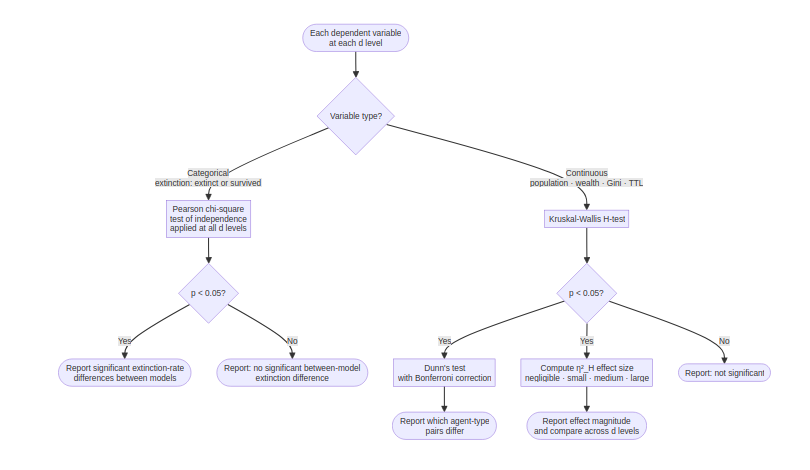
\includegraphics[width=\textwidth]{../../figures/stats.png}
			\end{figure}

			\textbf{Kruskal-Wallis \(H\)-Test.}
			To test whether the three ethical decision models produced significantly different societal outcomes within each resource configuration, the Kruskal-Wallis $H$-test was applied to each continuous dependent variable \citep{Kruskal1952}. The Kruskal-Wallis test is a non-parametric one-way analysis of variance by ranks that evaluates whether $k$ independent groups were drawn from populations with the same distribution. It jointly ranks all observations, computes the mean rank for each group, and derives a test statistic $H$ that is approximately chi-square distributed with $k - 1$ degrees of freedom when each group contains at least five observations \citep{Kruskal1952}.

			The test requires four assumptions: (1) all observations within and across groups are mutually independent; (2) the dependent variable is measured on at least an ordinal scale; (3) the distributions of all groups share the same shape, so that the test compares group medians rather than arbitrary distributional parameters \citep{Conover1999}; and (4) each group contains at least five observations so that the chi-square approximation of $H$ is valid \citep{Kruskal1952}. All four assumptions were satisfied in this study. Independence was ensured because each of the 100 seeds per condition was initialized from a distinct random state and no state was shared across conditions. The dependent variables are continuous ratio-scale measures, satisfying the ordinal requirement. The shape assumption was considered approximately met because all three groups within a given $d$ level were generated under identical simulation parameters, differing only in the ethical decision model. The minimum sample size requirement was satisfied in all cases: for metrics where extinct seeds were included (final population), each group contained exactly 100 observations; for metrics where extinct seeds were excluded (Gini coefficient, mean TTL, mean agent wealth, societal wealth at the distributed configuration ($d = 14$)), the altruistic and egoistic groups at the distributed configuration ($d = 14$) contained approximately 56 and 53 observations respectively, well above the minimum of five required for the chi-square approximation \citep{Kruskal1952}.

			The Kruskal-Wallis test was selected over the parametric one-way analysis of variance (ANOVA) for three reasons. First, ANOVA requires that the dependent variable be approximately normally distributed within each group. Simulation output variables such as final population counts are bounded below by zero, are right-skewed when extinction occurs frequently, and may accumulate a mass of zero values in conditions with high extinction rates, making the normality assumption untenable \citep{Field2013}. The Gini coefficient is similarly bounded in $[0, 1]$, which precludes the symmetric tails assumed by the normal distribution. Second, ANOVA assumes homoscedasticity, or equal within-group variances, across the groups being compared, an assumption that cannot be guaranteed across ethical models with qualitatively different behavioral dynamics. Third, because the distributional shape of simulation outputs was not known a priori, a distribution-free method that makes no parametric assumptions about the population was methodologically more defensible. A significance threshold of $\alpha = 0.05$ was applied to all inferential tests.

			\textbf{Post-hoc Dunn's Test with Bonferroni Correction.}
			The Kruskal-Wallis test is an omnibus procedure: a significant result establishes only that at least one group differs from the others without identifying which specific pairs are responsible. When the Kruskal-Wallis test yielded $p < 0.05$ for a given metric and $d$ level, pairwise post-hoc comparisons were conducted using Dunn's test \citep{Dunn1964}. Dunn's test is the recommended post-hoc procedure following a significant Kruskal-Wallis result because it operates within the same rank-sum framework as the omnibus test: each pairwise comparison computes a $z$-statistic from the difference in mean ranks between two groups, standardized by the pooled standard error derived from the same joint ranking used in the omnibus test \citep{Dunn1964}. This maintains consistency between the omnibus and pairwise analyses and avoids the interpretive mismatch that arises when parametric post-hoc tests are applied after a non-parametric omnibus result.

			To control the family-wise error rate (FWER), the probability of committing at least one Type~I error across the set of simultaneous pairwise comparisons, Bonferroni correction was applied to all pairwise $p$-values \citep{Bonferroni1936}. With $k = 3$ groups, there are $\binom{3}{2} = 3$ pairwise comparisons per metric per $d$ level. The Bonferroni procedure divides the nominal significance level by the number of comparisons, yielding an adjusted per-comparison threshold of $\alpha^{*} = 0.05 / 3 \approx 0.017$ \citep{Dunn1961}. Although Bonferroni correction is conservative, treating all comparisons as statistically independent and therefore increasing the risk of Type~II errors, its stringency was considered appropriate for a confirmatory hypothesis test with a small number of comparisons.

			\textbf{Effect Size (\(\eta^2_H\)).}
			Statistical significance alone does not convey the practical magnitude of an observed difference. To quantify the strength of the group effect for each Kruskal-Wallis test, $\eta^2_H$ was computed using the formula proposed by \citet{Tomczak2014}:

			\begin{equation}
				\eta^2_H = \frac{H - k + 1}{n - k},
			\end{equation}

			\noindent where $H$ is the Kruskal-Wallis test statistic, $k$ is the number of groups, and $n$ is the total number of observations. $\eta^2_H$ is bounded in $[0, 1]$ and represents the proportion of variance in ranks attributable to group membership, making it conceptually analogous to $\eta^2$ in ANOVA \citep{Cohen1988}. Effect sizes were interpreted using the thresholds recommended by \citet{Tomczak2014}: negligible ($\eta^2_H < 0.01$), small ($0.01 \leq \eta^2_H < 0.06$), medium ($0.06 \leq \eta^2_H < 0.14$), or large ($\eta^2_H \geq 0.14$).

			To address RQ4 ($H_{0,4}$ versus $H_{a,4}$), the $\eta^2_H$ values obtained at the concentrated ($d = 0$), moderately concentrated ($d = 7$), and distributed ($d = 14$) configurations were compared directionally across the three resource configurations for each outcome metric. Variation in $\eta^2_H$ across configurations was taken as evidence that the magnitude of performance differences between ethical decision models depends on resource geography.

			\textbf{Chi-Square Test of Independence.}
			The binary extinction outcome, whether the population went extinct before completing 5000 timesteps, is a categorical variable and cannot be analyzed with the Kruskal-Wallis test. To test whether the proportion of extinct runs differed across the three agent-type conditions, extinction counts were arranged into a $3 \times 2$ contingency table (three agent types $\times$ two outcomes: extinct or survived) and a Pearson chi-square test of independence was applied \citep{Pearson1900}. The chi-square test was applied at all three resource configurations. At the distributed configuration ($d = 14$), inter-model extinction rates differed substantially (1\%, 44\%, 47\%), and the test was expected to be significant. At the moderately concentrated ($d = 7$) and concentrated ($d = 0$) configurations, extinction rates were non-zero across all models but closer in magnitude (8--14\% at the moderately concentrated ($d = 7$); 14--20\% at the concentrated ($d = 0$)), and the test was applied to determine whether those differences exceeded chance.

			The chi-square test of independence requires three assumptions: (1) the observations are independent of one another; (2) the outcome categories are mutually exclusive and exhaustive; and (3) the expected frequency in each cell of the contingency table is at least 5 \citep{Cochran1954}. Independence was satisfied because each seed was initialized from a distinct random state with no shared simulation history. Mutual exclusivity was satisfied because each run either terminated in extinction or survived to 5000 timesteps with no overlap between these outcomes. The expected cell count assumption was verified prior to interpretation, confirming that all cells in the applicable contingency table met the minimum expected frequency of 5 \citep{Cochran1954}.
		
		\subsection{Research Design Summary}
			Table~\ref{table:research-design} summarizes how each study objective was operationalized through the experimental design and addressed through specific statistical procedures. The simulation conditions provided the data; descriptive and inferential statistics translated that data into answers to each research question. Each objective maps to one or more dependent variables and one or more statistical tests.

			\begin{table}[H]
			\vspace{2ex}
			\centering
			\caption{Research Design Summary: Objectives, Measures, and Procedures}
			\label{table:research-design}
			\footnotesize
			\renewcommand{\arraystretch}{1.5}
			\begin{tabular}{
				>{\raggedright\arraybackslash}p{0.4cm}
				>{\raggedright\arraybackslash}p{3.2cm}
				>{\raggedright\arraybackslash}p{3.2cm}
				>{\raggedright\arraybackslash}p{6.2cm}
			}
			\hline\hline
			\textbf{No.} & \textbf{Objective} & \textbf{Outcome Measures} & \textbf{Statistical Test} \\
			\hline
			1 &
				Compare societal outcomes of the three ethical models across all three resource configurations ($d = 14$, $d = 7$, $d = 0$). &
				Final population, mean agent wealth, societal wealth, Gini coefficient, mean TTL, extinction rate. &
				Kruskal-Wallis $H$-test per metric at each $d$ level; Dunn's test with Bonferroni correction if $p < 0.05$; $\eta^2_H$ effect size; Pearson chi-square for extinction rate at each $d$ level. \\

			2 &
				Determine whether the utilitarian advantage is maintained, strengthened, or weakened as resource peaks converge. &
				$\eta^2_H$ per metric per $d$ level (derived from Objective~1). &
				Directional comparison of $\eta^2_H$ across $d = 0$, $d = 7$, $d = 14$; variation in effect size taken as evidence against $H_{0,4}$. \\

			3 &
				Identify which resource layout produces the most distinct differences in outcomes among the three agent types. &
				$\eta^2_H$ per metric across all three $d$ levels (derived from Objectives~1 and~2). &
				Synthesis interpretation of $\eta^2_H$ patterns; no additional inferential test required. \\

			4 &
				Record and report wall-clock execution time of individual simulation runs as a computational benchmark. &
				Execution time per run (seconds). &
				Descriptive statistics: mean, standard deviation, and interquartile range per condition. No inferential test. \\
			\hline
			\end{tabular}
			\end{table}

		\section{RESULTS AND DISCUSSION}

		\subsection{Objective 1: Societal Outcomes Across Resource Configurations}

Table~\ref{table:desc-d14} summarizes the key outcomes for the distributed configuration. Full descriptive statistics for all metrics are reported in Table~\ref{table:app-desc-all} in the Appendix. As shown in Table~\ref{table:extinction-rate}, the utilitarian model went extinct in 1\% of the 100 observed seeds, while the altruistic and egoistic models went extinct in 44\% and 47\% of seeds, respectively. The utilitarian model achieved the highest median final population (1,425.5; IQR = 178.3); altruistic and egoistic produced medians of 395 (IQR = 1,046.0) and 368.5 (IQR = 1,066.8).

		\begin{table}[H]
		\vspace{2ex}
		\centering
		\caption{Key Outcomes for the Distributed Configuration ($d = 14$, $n = 100$ per model)}
		\label{table:desc-d14}
		\footnotesize
		\renewcommand{\arraystretch}{1.3}
		\begin{tabular}{l >{\raggedright\arraybackslash}p{3.2cm} r}
		\hline\hline
		\textbf{Model} & \textbf{Final Population} \textit{Mdn (IQR)} & \textbf{Extinct (\%)} \\
		\hline
		Utilitarian & 1,425.5 (178.3)  & 1.0  \\
		Altruistic  & 395 (1,046.0)    & 44.0 \\
		Egoistic    & 368.5 (1,066.8)  & 47.0 \\
		\hline
		\end{tabular}
		\par\smallskip
		{\footnotesize\noindent\textit{Note.} Extinction rate = proportion of seeds reaching zero population before timestep 5,000. Societal wealth ($\eta^2_H = 0.207$, large) and mean TTL ($\eta^2_H = 0.146$, large) differed significantly in favour of the utilitarian model; Gini coefficient and mean agent wealth did not differ significantly. Full statistics in Table~\ref{table:app-desc-all}.}
		\end{table}

The Kruskal-Wallis test yielded a significant group difference in final population ($H = 142.774$, $df = 2$, $p < 0.001$, $\eta^2_H = 0.474$, large effect; see Table~\ref{table:app-kw}). Pairwise Dunn tests (Table~\ref{table:app-dunn}) confirmed that the utilitarian model produced a significantly larger final population than both the altruistic ($p < 0.001$) and egoistic ($p < 0.001$) models; altruistic and egoistic models did not differ significantly from each other. The Pearson chi-square test confirmed that extinction rates differed across models ($\chi^2 = 62.301$, $df = 2$, $p < 0.001$). Final societal wealth also differed significantly ($H = 63.611$, $p < 0.001$, $\eta^2_H = 0.207$, large effect), with pairwise Dunn tests confirming that the utilitarian model produced higher societal wealth than both altruistic ($p < 0.001$) and egoistic ($p < 0.001$) models. Mean time to live likewise differed significantly ($H = 45.350$, $p < 0.001$, $\eta^2_H = 0.146$, large effect), with utilitarian agents maintaining higher median TTL than both altruistic ($p < 0.001$) and egoistic ($p < 0.001$) models, driven by the large proportions of extinct seeds in the non-utilitarian conditions contributing near-zero TTL values. Gini coefficient did not reach significance ($H = 5.617$, $p = 0.060$, $\eta^2_H = 0.012$), and mean agent wealth was not significant ($H = 0.377$, $p = 0.828$, $\eta^2_H = 0.000$). $H_{0,1}$ was rejected for final population, extinction rate, societal wealth, and mean time to live; retained for Gini coefficient and mean agent wealth.

		\begin{table}[H]
		\vspace{2ex}
		\centering
		\caption{Extinction Rate by Agent Type and Resource Configuration ($n = 100$ per condition)}
		\label{table:extinction-rate}
		\footnotesize
		\renewcommand{\arraystretch}{1.3}
		\begin{tabular}{l r r r}
		\hline\hline
		\textbf{Model} & \textbf{$d = 14$ (distributed)} & \textbf{$d = 7$ (moderately concentrated)} & \textbf{$d = 0$ (concentrated)} \\
		\hline
		Utilitarian &  1.0\% & 14.0\% & 14.0\% \\
		Altruistic  & 44.0\% &  9.0\% & 20.0\% \\
		Egoistic    & 47.0\% &  8.0\% & 17.0\% \\
		\hline
		\end{tabular}
		\par\smallskip
		{\footnotesize\noindent\textit{Note.} Extinction = population reached zero before timestep 5,000. Chi-square test significant only at the distributed configuration ($d = 14$) ($\chi^2 = 62.301$, $p < 0.001$); extinction differences at the moderately concentrated ($d = 7$, $p = 0.328$) and concentrated ($d = 0$, $p = 0.528$) configurations were not significant.}
		\end{table}

The present study replicated the central finding of \citet{KremerHerman2024} that utilitarian societies outperform altruistic and egoistic societies under distributed resource conditions. Those authors reported that utilitarian societies consistently achieved the largest populations, the greatest accumulated wealth, and the longest survival; in the present study, the utilitarian model achieved a significantly higher final population ($\eta^2_H = 0.474$, large effect) and went extinct in only 1\% of the 100 observed seeds, while altruistic and egoistic societies went extinct in 44\% and 47\% of seeds, respectively, with pairwise Dunn tests confirming that both non-utilitarian models fell significantly below the utilitarian in final population (both $p < 0.001$) while remaining statistically indistinguishable from each other. The population and survival advantage of the utilitarian model at the distributed configuration ($d = 14$) thus replicates the comparative ranking reported by \citet{KremerHerman2024}.

With $n = 100$ seeds, the present study converges closely with \citet{KremerHerman2024} on the societal wealth metric. Their Figure~8 shows utilitarian societies accumulating substantially more total wealth than altruistic and egoistic societies; in the present study, the Kruskal-Wallis test on final societal wealth yielded a significant group effect ($H = 63.611$, $p < 0.001$, $\eta^2_H = 0.207$, large effect), with pairwise Dunn tests confirming that the utilitarian model produced higher societal wealth than both altruistic ($p < 0.001$) and egoistic ($p < 0.001$) models. This result is consistent with the interpretation of \citet{KremerHerman2024} that societal wealth tracks population: with 44\% and 47\% of altruistic and egoistic seeds becoming extinct, the surviving utilitarian societies supported more agents and consequently accumulated greater total resources. Gini coefficient remained non-significant ($H = 5.617$, $p = 0.060$, $\eta^2_H = 0.012$); as \citet{KremerHerman2024} did not report a Gini analysis in their homogeneous society experiments, this constitutes a novel measurement. Mean agent wealth was not significant ($H = 0.377$, $p = 0.828$, $\eta^2_H = 0.000$), indicating that per-agent resource accumulation did not differ across models once population-level extinction differences are accounted for.

The high outcome variability of altruistic and egoistic models reflects well-documented behavioral instabilities at the agent level. The altruistic model's large IQR (1,046.0) and 44\% extinction rate are consistent with the bimodal dynamic described by \citet{KremerHerman2024}, in which altruistic agents that exclude their own welfare from cell scoring progressively deplete their resource stores when surrounded by equally self-sacrificing neighbors; the egoistic model's 47\% extinction rate and IQR of 1,066.8 align with the ``murderous period'' of \citet{KremerHerman2024} and with \citet{Xiang2008}, who found that selfish agent populations passed through an unstable transitional phase of sharp fluctuation before settling at a new equilibrium. The bimodal volatility in both non-utilitarian models underscores that extreme ethical orientations carry elevated stochastic risk under distributed resource conditions.

Mean time to live differed significantly ($H = 45.350$, $p < 0.001$, $\eta^2_H = 0.146$, large effect), with utilitarian agents maintaining the highest median TTL (18.250 timesteps) compared to altruistic (12.255) and egoistic (9.920) models. This result is primarily driven by the high extinction rates of non-utilitarian conditions: the large proportions of extinct seeds in altruistic (44\%) and egoistic (47\%) conditions contribute near-zero TTL values to their distributions, depressing the medians and producing the large IQRs of 18.258 and 18.948 timesteps respectively. Pairwise Dunn tests confirmed that both altruistic ($p < 0.001$) and egoistic ($p < 0.001$) models differed significantly from the utilitarian, while altruistic and egoistic did not differ from each other. The ethical model at the distributed configuration ($d = 14$) therefore appears to determine whether a society clears the early survival threshold, and this survival penalty is reflected in the TTL metric through the inclusion of near-zero values from extinct runs.

Overall, the distributed configuration ($d = 14$) results establish a strong replication of \citet{KremerHerman2024}: the utilitarian model holds a clear advantage across population ($\eta^2_H = 0.474$, large), societal wealth ($\eta^2_H = 0.207$, large), and mean time to live ($\eta^2_H = 0.146$, large), with substantially lower extinction rates (1\% vs.\ 44\% and 47\% for altruistic and egoistic). Gini coefficient and mean agent wealth remained non-significant, consistent with the interpretation that the utilitarian advantage is concentrated in collective survival outcomes rather than in per-agent resource accumulation. The high volatility of altruistic and egoistic outcomes reflects behavioral mechanisms previously identified in the literature, and the large TTL effect reflects the same extinction-driven bimodality rather than differences in individual longevity among surviving agents.


Figures~\ref{fig:pop-timeseries-d14}--\ref{fig:pop-timeseries-d0} show the mean population trajectory for all three agent types across all three configurations. The performance reversal is visible in the transition from the distributed ($d = 14$) to the moderately concentrated ($d = 7$) and concentrated ($d = 0$) configurations: the utilitarian trajectory, which leads at the distributed configuration ($d = 14$), falls to the bottom at the moderately concentrated ($d = 7$) and concentrated ($d = 0$) configurations while the altruistic and egoistic trajectories converge near the top. Table~\ref{table:desc-d7-d0} summarizes the key outcomes; full statistics are in Table~\ref{table:app-desc-all}.

		\begin{figure}[H]
		\caption{Mean population over time ($\pm$1 SD across 100 seeds), distributed ($d = 14$).}
		\label{fig:pop-timeseries-d14}
		\centering
		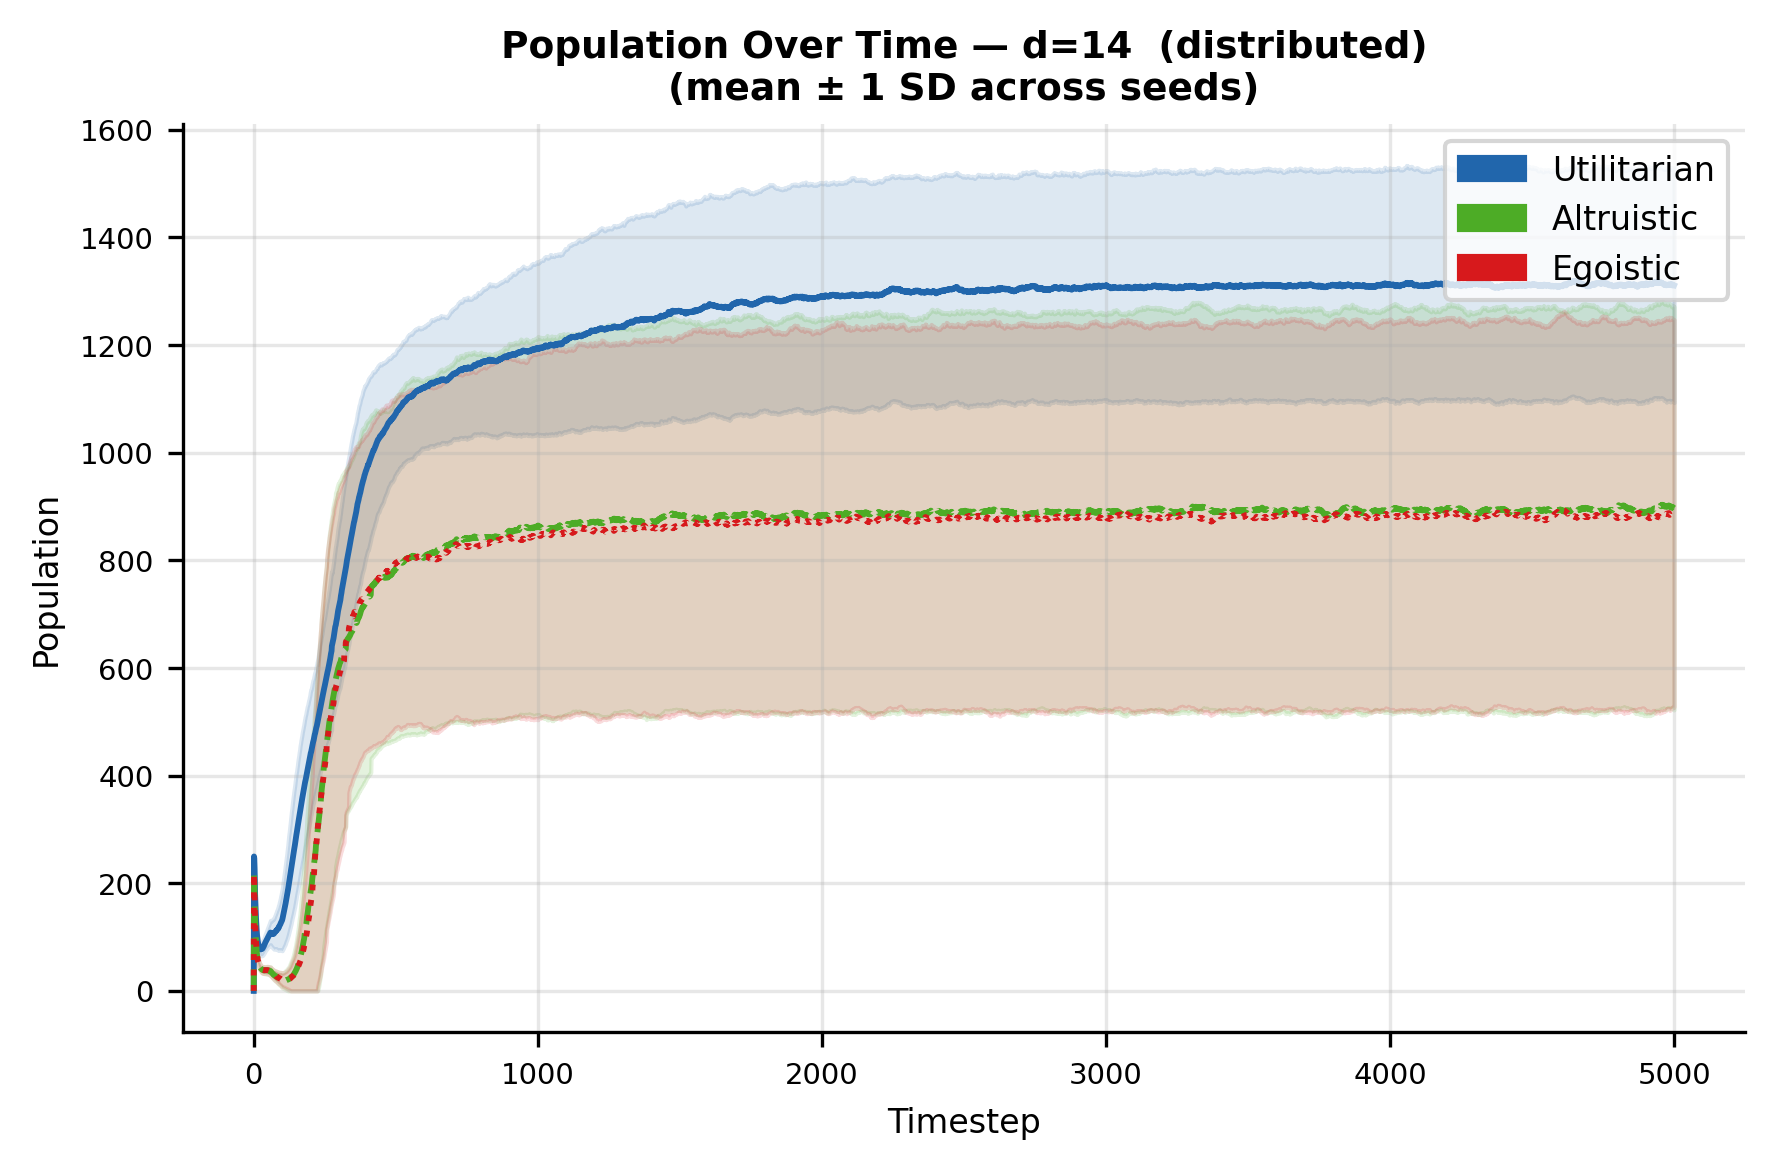
\includegraphics[width=0.8\textwidth]{../../figures/01_population_timeseries_d14.png}
		\par\smallskip
		{\footnotesize\noindent\textit{Note.} Shaded bands = $\pm$1 SD. Blue solid = Utilitarian; green dashed = Altruistic; red dotted = Egoistic.}
		\end{figure}

		\begin{figure}[H]
		\caption{Mean population over time ($\pm$1 SD across 100 seeds), moderately concentrated ($d = 7$).}
		\label{fig:pop-timeseries-d7}
		\centering
		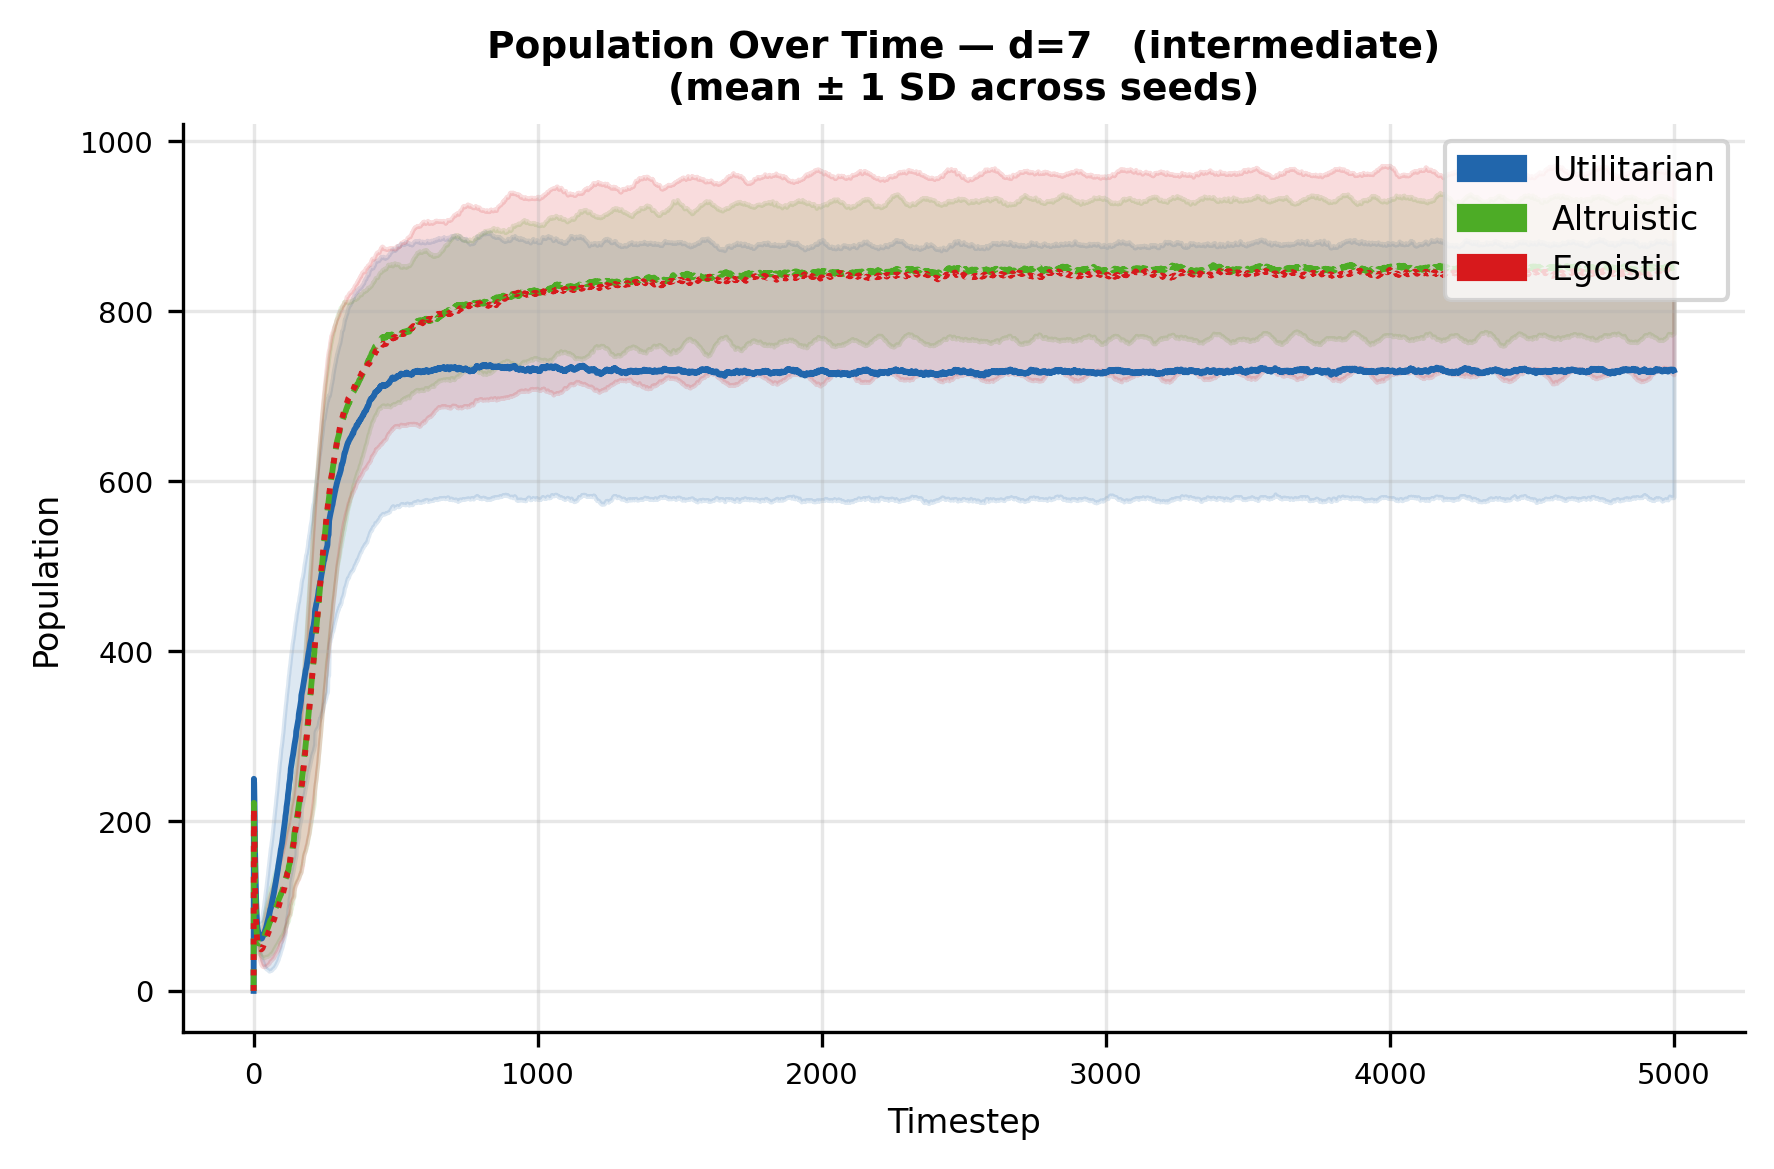
\includegraphics[width=0.8\textwidth]{../../figures/01_population_timeseries_d7.png}
		\par\smallskip
		{\footnotesize\noindent\textit{Note.} Shaded bands = $\pm$1 SD. Blue solid = Utilitarian; green dashed = Altruistic; red dotted = Egoistic.}
		\end{figure}

		\begin{figure}[H]
		\caption{Mean population over time ($\pm$1 SD across 100 seeds), concentrated ($d = 0$).}
		\label{fig:pop-timeseries-d0}
		\centering
		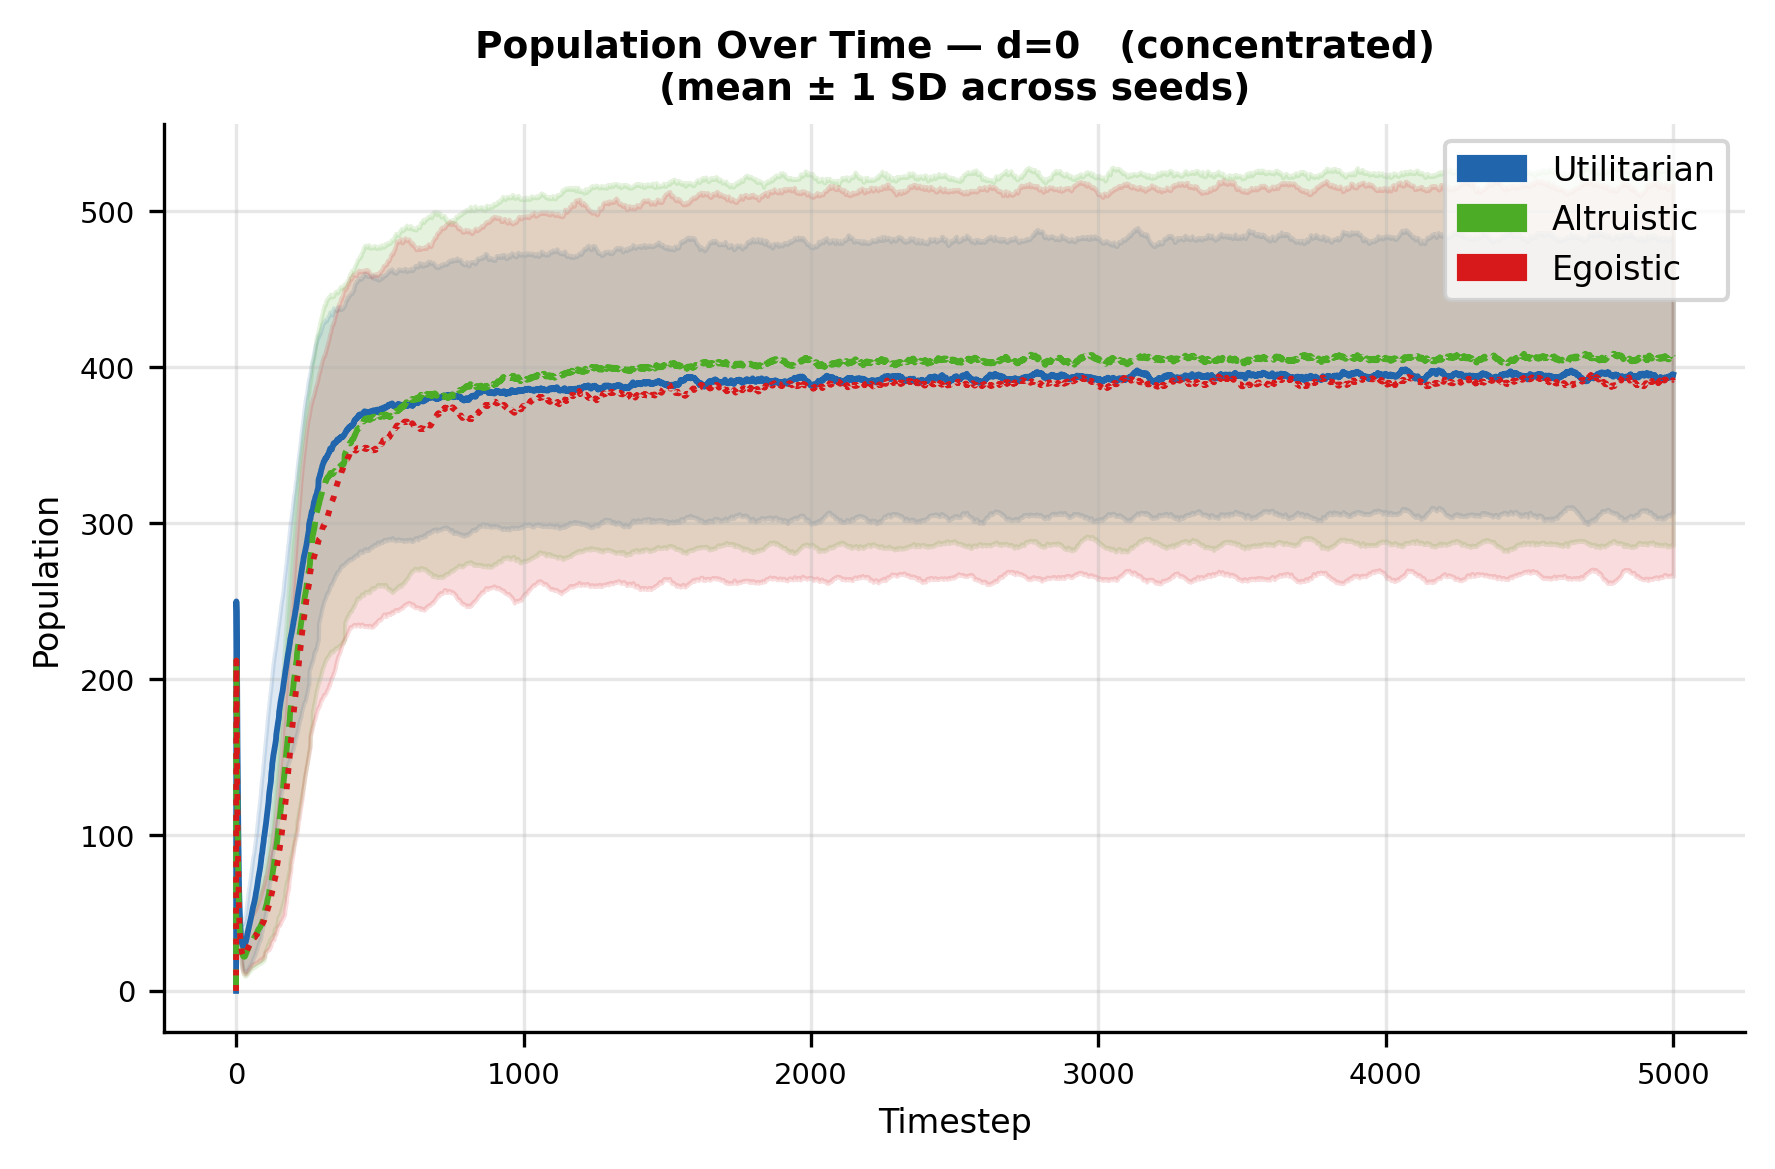
\includegraphics[width=0.8\textwidth]{../../figures/01_population_timeseries_d0.png}
		\par\smallskip
		{\footnotesize\noindent\textit{Note.} Shaded bands = $\pm$1 SD. Blue solid = Utilitarian; green dashed = Altruistic; red dotted = Egoistic.}
		\end{figure}

		\begin{table}[H]
		\vspace{2ex}
		\centering
		\caption{Key Societal Outcomes Across All Three Resource Configurations ($n = 100$ per model)}
		\label{table:desc-d7-d0}
		\footnotesize
		\renewcommand{\arraystretch}{1.3}
		\begin{tabular}{l r r r}
		\hline\hline
		\textbf{Model} & \textbf{Population} \textit{Mdn (IQR)} & \textbf{Societal Wealth} \textit{Mdn (IQR)} & \textbf{Gini} \textit{Mdn (IQR)} \\
		\hline
		\multicolumn{4}{l}{\textit{Distributed ($d = 14$); extinction rate: Utilitarian 1\%, Altruistic 44\%, Egoistic 47\%}} \\
		\hline
		Utilitarian & 1,425.5 (178.3)  & 68,210 (6,861)   & 0.166 (0.020) \\
		Altruistic  & 395 (1,046.0)    & 41,349 (65,359)  & 0.163 (0.248) \\
		Egoistic    & 368.5 (1,066.8)  & 28,643 (67,497)  & 0.152 (0.220) \\
		\hline
		\multicolumn{4}{l}{\textit{Moderately concentrated ($d = 7$); extinction rate: Utilitarian 14\%, Altruistic 9\%, Egoistic 8\%}} \\
		\hline
		Utilitarian & 767.5 (51.3) & 42,259 (3,370) & 0.208 (0.025) \\
		Altruistic  & 863 (26.3) & 40,985 (3,172) & 0.159 (0.014) \\
		Egoistic    & 867 (30.0) & 41,290 (4,003) & 0.159 (0.015) \\
		\hline
		\multicolumn{4}{l}{\textit{Concentrated ($d = 0$); extinction rate: Utilitarian 14\%, Altruistic 20\%, Egoistic 17\%}} \\
		\hline
		Utilitarian & 422 (42.0)   & 20,525 (2,537) & 0.189 (0.030) \\
		Altruistic  & 449 (342.0)  & 21,113 (6,356) & 0.163 (0.034) \\
		Egoistic    & 443 (317.5)  & 22,268 (4,371) & 0.164 (0.045) \\
		\hline
		\end{tabular}
		\par\smallskip
		{\footnotesize\noindent\textit{Note.} Societal wealth and population medians at the distributed configuration ($d = 14$) are influenced by large proportions of extinct seeds. Mean TTL differed significantly at the distributed configuration ($d = 14$) (large effect, extinction-driven) and the moderately concentrated ($d = 7$) (small effect; see text) but not at the concentrated ($d = 0$). Full statistics including mean TTL and mean agent wealth in Table~\ref{table:app-desc-all}.}
		\end{table}

At the moderately concentrated configuration ($d = 7$), Kruskal-Wallis tests identified significant group differences in final population ($H = 117.783$, $p < 0.001$, $\eta^2_H = 0.390$, large), Gini coefficient ($H = 88.262$, $p < 0.001$, $\eta^2_H = 0.290$, large), and mean agent wealth ($H = 64.414$, $p < 0.001$, $\eta^2_H = 0.210$, large). Final societal wealth ($H = 6.338$, $p = 0.042$, $\eta^2_H = 0.015$, small) and mean time to live ($H = 6.639$, $p = 0.036$, $\eta^2_H = 0.016$, small) were also significant but with small effects. Pairwise Dunn tests (Table~\ref{table:app-dunn}) confirmed that, for population, Gini, and mean wealth, the utilitarian model differed significantly from both altruistic and egoistic models (all $p < 0.001$); for societal wealth, the utilitarian model differed significantly from the altruistic model ($p = 0.038$) but not from the egoistic model ($p = 0.375$); for mean TTL, a significant difference was identified between egoistic and utilitarian models ($p = 0.048$), with egoistic agents maintaining the higher mean TTL, while altruistic agents did not differ significantly from either; altruistic and egoistic models did not differ from each other on any metric. Extinction rates did not differ significantly across models at the moderately concentrated configuration ($d = 7$, $\chi^2 = 2.230$, $p = 0.328$). $H_{0,2}$ was rejected for final population, Gini coefficient, societal wealth, mean agent wealth, and mean time to live.

At the concentrated configuration ($d = 0$), significant differences were found for final population ($H = 20.210$, $p < 0.001$, $\eta^2_H = 0.061$, medium), final societal wealth ($H = 15.121$, $p < 0.001$, $\eta^2_H = 0.044$, small), and Gini coefficient ($H = 30.180$, $p < 0.001$, $\eta^2_H = 0.095$, medium). Pairwise Dunn tests confirmed that for final population, both altruistic ($p < 0.001$) and egoistic ($p = 0.001$) models differed significantly from the utilitarian model, with altruistic and egoistic producing higher median populations; for societal wealth, only egoistic differed significantly from the utilitarian ($p < 0.001$, Ego $>$ Util), while altruistic did not ($p = 0.219$); for Gini, both altruistic ($p < 0.001$) and egoistic ($p < 0.001$) differed significantly from the utilitarian, which maintained the higher Gini. Altruistic and egoistic models did not differ significantly from each other on any metric (all $p > 0.10$). Crucially, the direction of population differences reversed relative to the distributed configuration ($d = 14$): at the concentrated configuration ($d = 0$), non-utilitarian models produced higher median populations than the utilitarian model, while the utilitarian model retained a higher Gini coefficient. For societal wealth, the reversal was partial: only egoistic agents accumulated significantly more total wealth than the utilitarian model. Mean time to live ($H = 2.487$, $p = 0.288$) and mean agent wealth ($H = 5.740$, $p = 0.057$) were not significant. Extinction rates did not differ significantly at the concentrated configuration ($d = 0$, $\chi^2 = 1.276$, $p = 0.528$). $H_{0,3}$ was rejected for final population, societal wealth, and Gini coefficient, and retained for mean time to live and mean agent wealth.

Figures~\ref{fig:boxplot-population}--\ref{fig:boxplot-meanwealth} display the full distribution of final outcome values across all nine conditions for visual comparison.

		\begin{figure}[H]
		\caption{Final population distribution by agent type and resource configuration ($n = 100$ per condition).}
		\label{fig:boxplot-population}
		\centering
		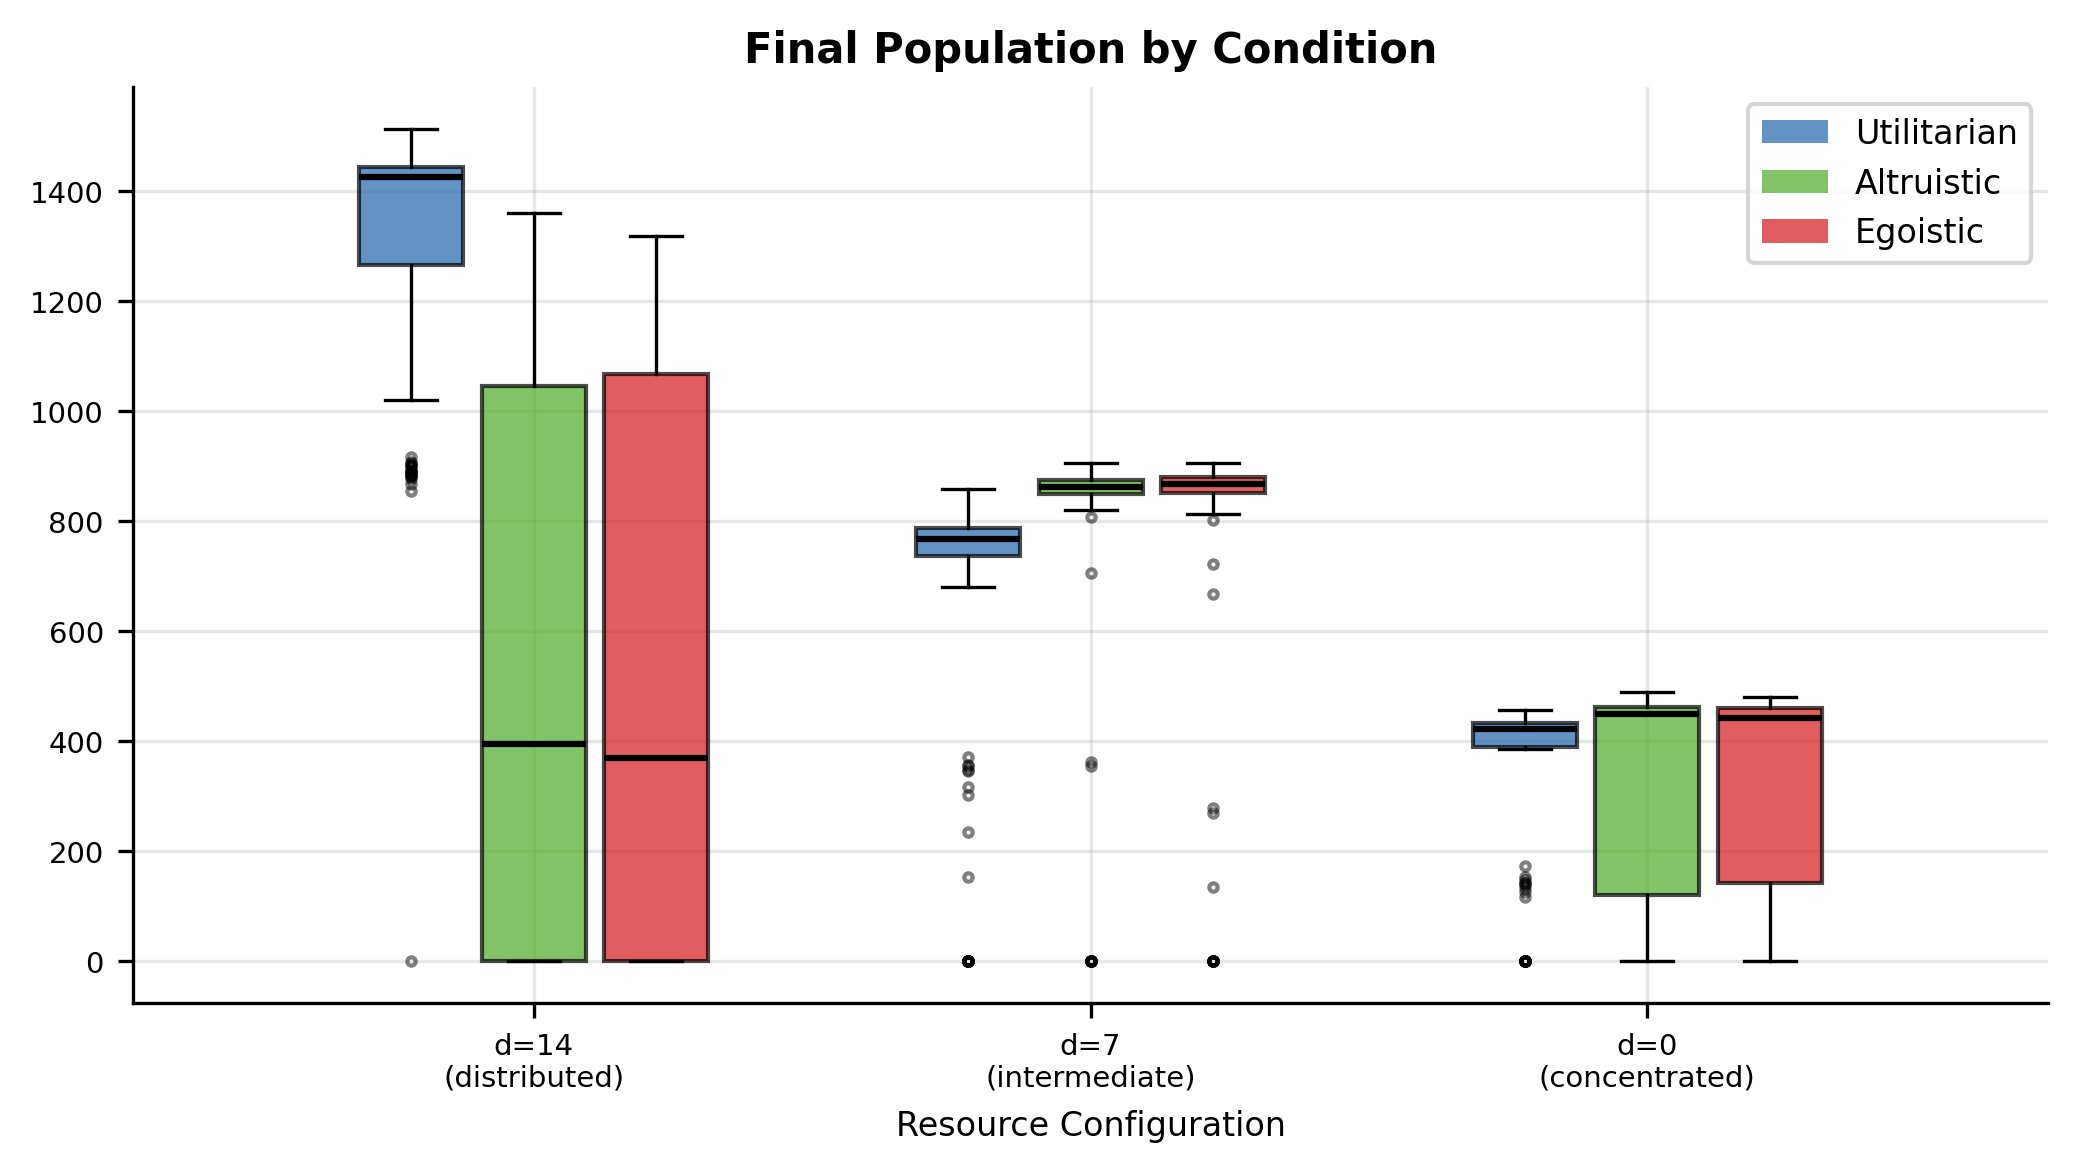
\includegraphics[width=0.85\textwidth]{../../figures/06_boxplot_finalPopulation.png}
		\par\smallskip
		{\footnotesize\noindent\textit{Note.} Each box spans the IQR across 100 seeds; the horizontal line is the median. Blue = Utilitarian, green = Altruistic, red = Egoistic.}
		\end{figure}

		\begin{figure}[H]
		\caption{Final societal wealth distribution by agent type and resource configuration ($n = 100$ per condition).}
		\label{fig:boxplot-wealth}
		\centering
		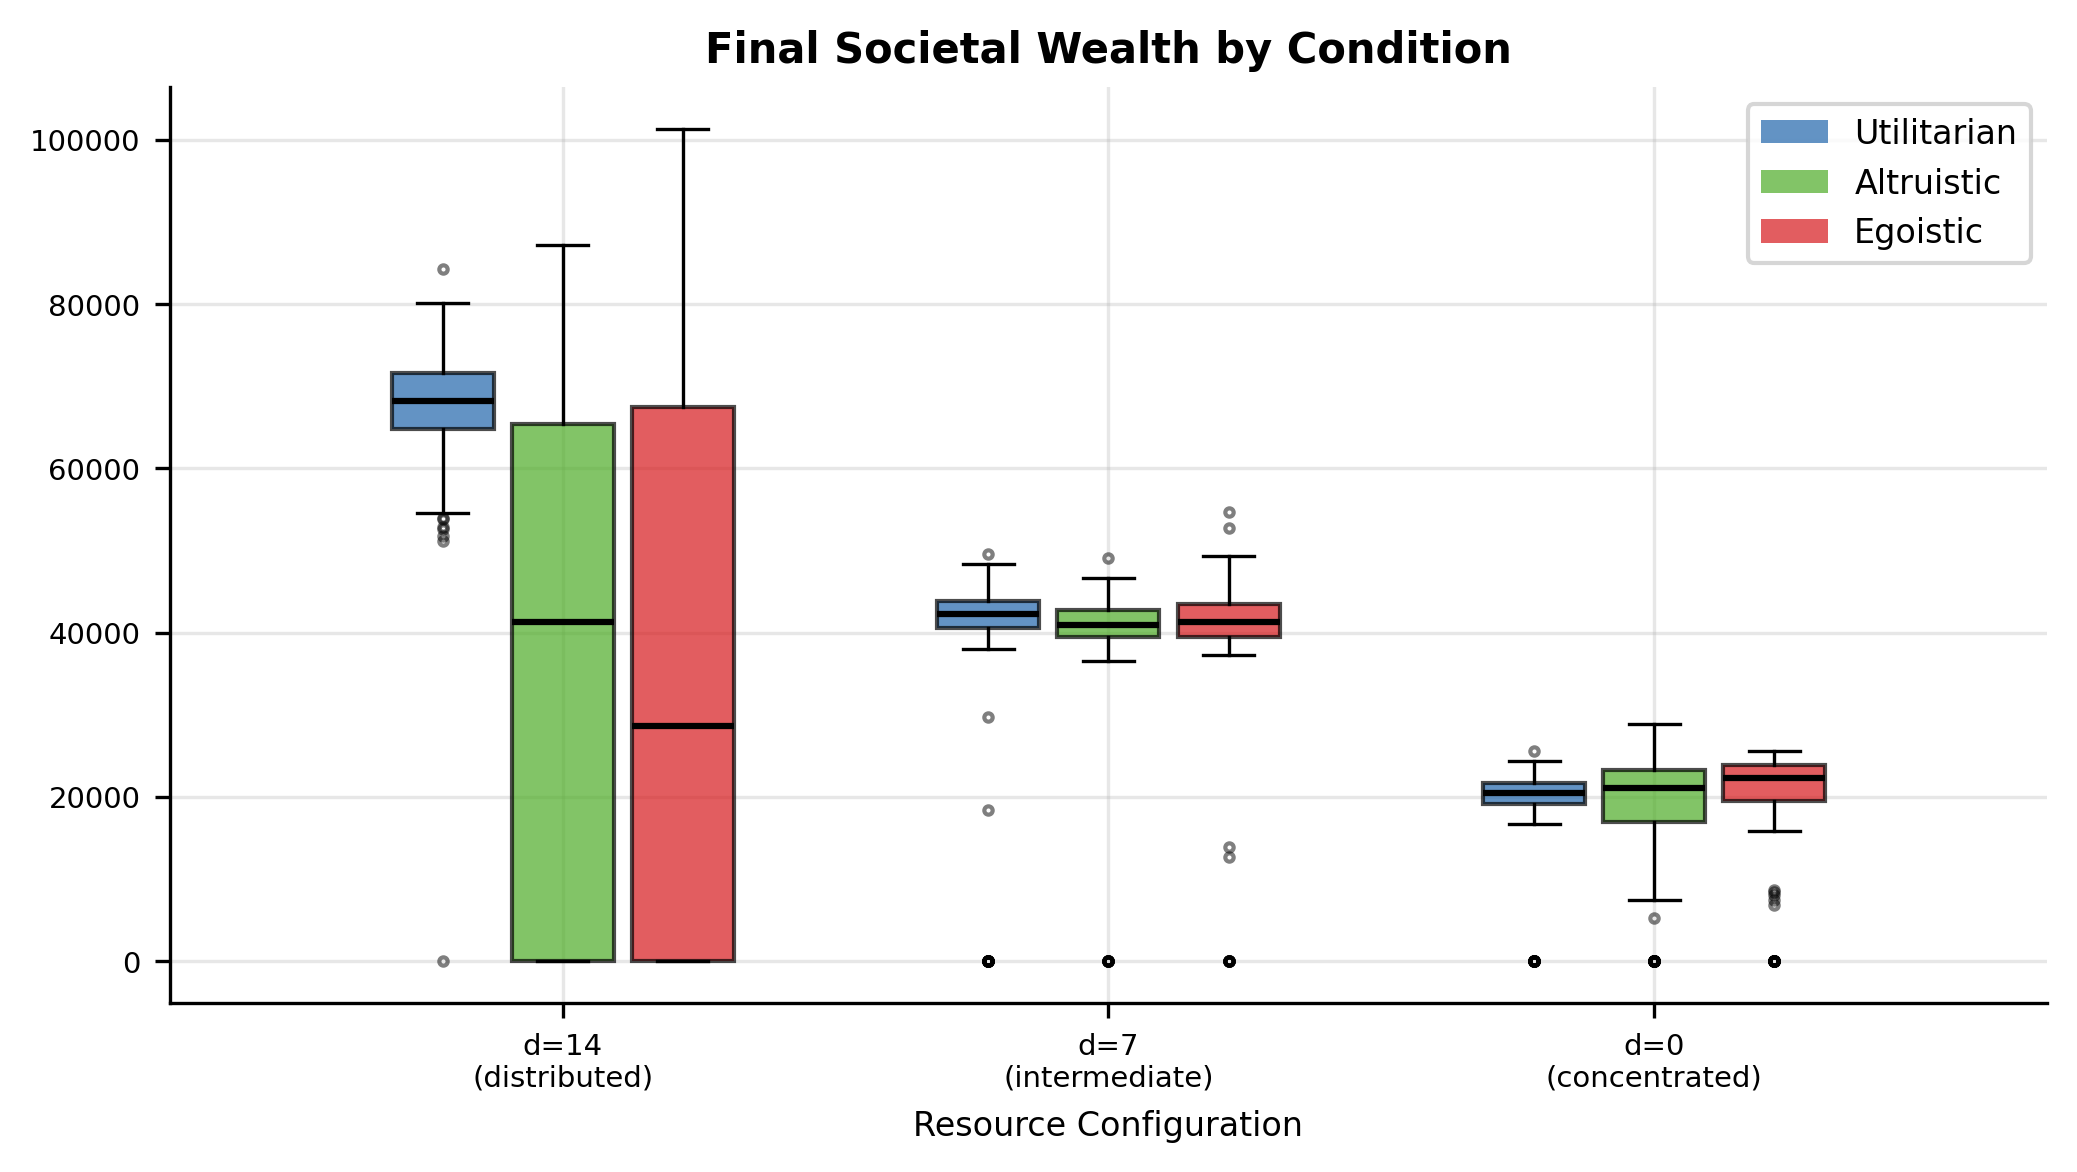
\includegraphics[width=0.85\textwidth]{../../figures/06_boxplot_finalSocietalWealth.png}
		\par\smallskip
		{\footnotesize\noindent\textit{Note.} Each box spans the IQR across 100 seeds; the horizontal line is the median. Blue = Utilitarian, green = Altruistic, red = Egoistic.}
		\end{figure}

		\begin{figure}[H]
		\caption{Final Gini coefficient distribution by agent type and resource configuration ($n = 100$ per condition).}
		\label{fig:boxplot-gini}
		\centering
		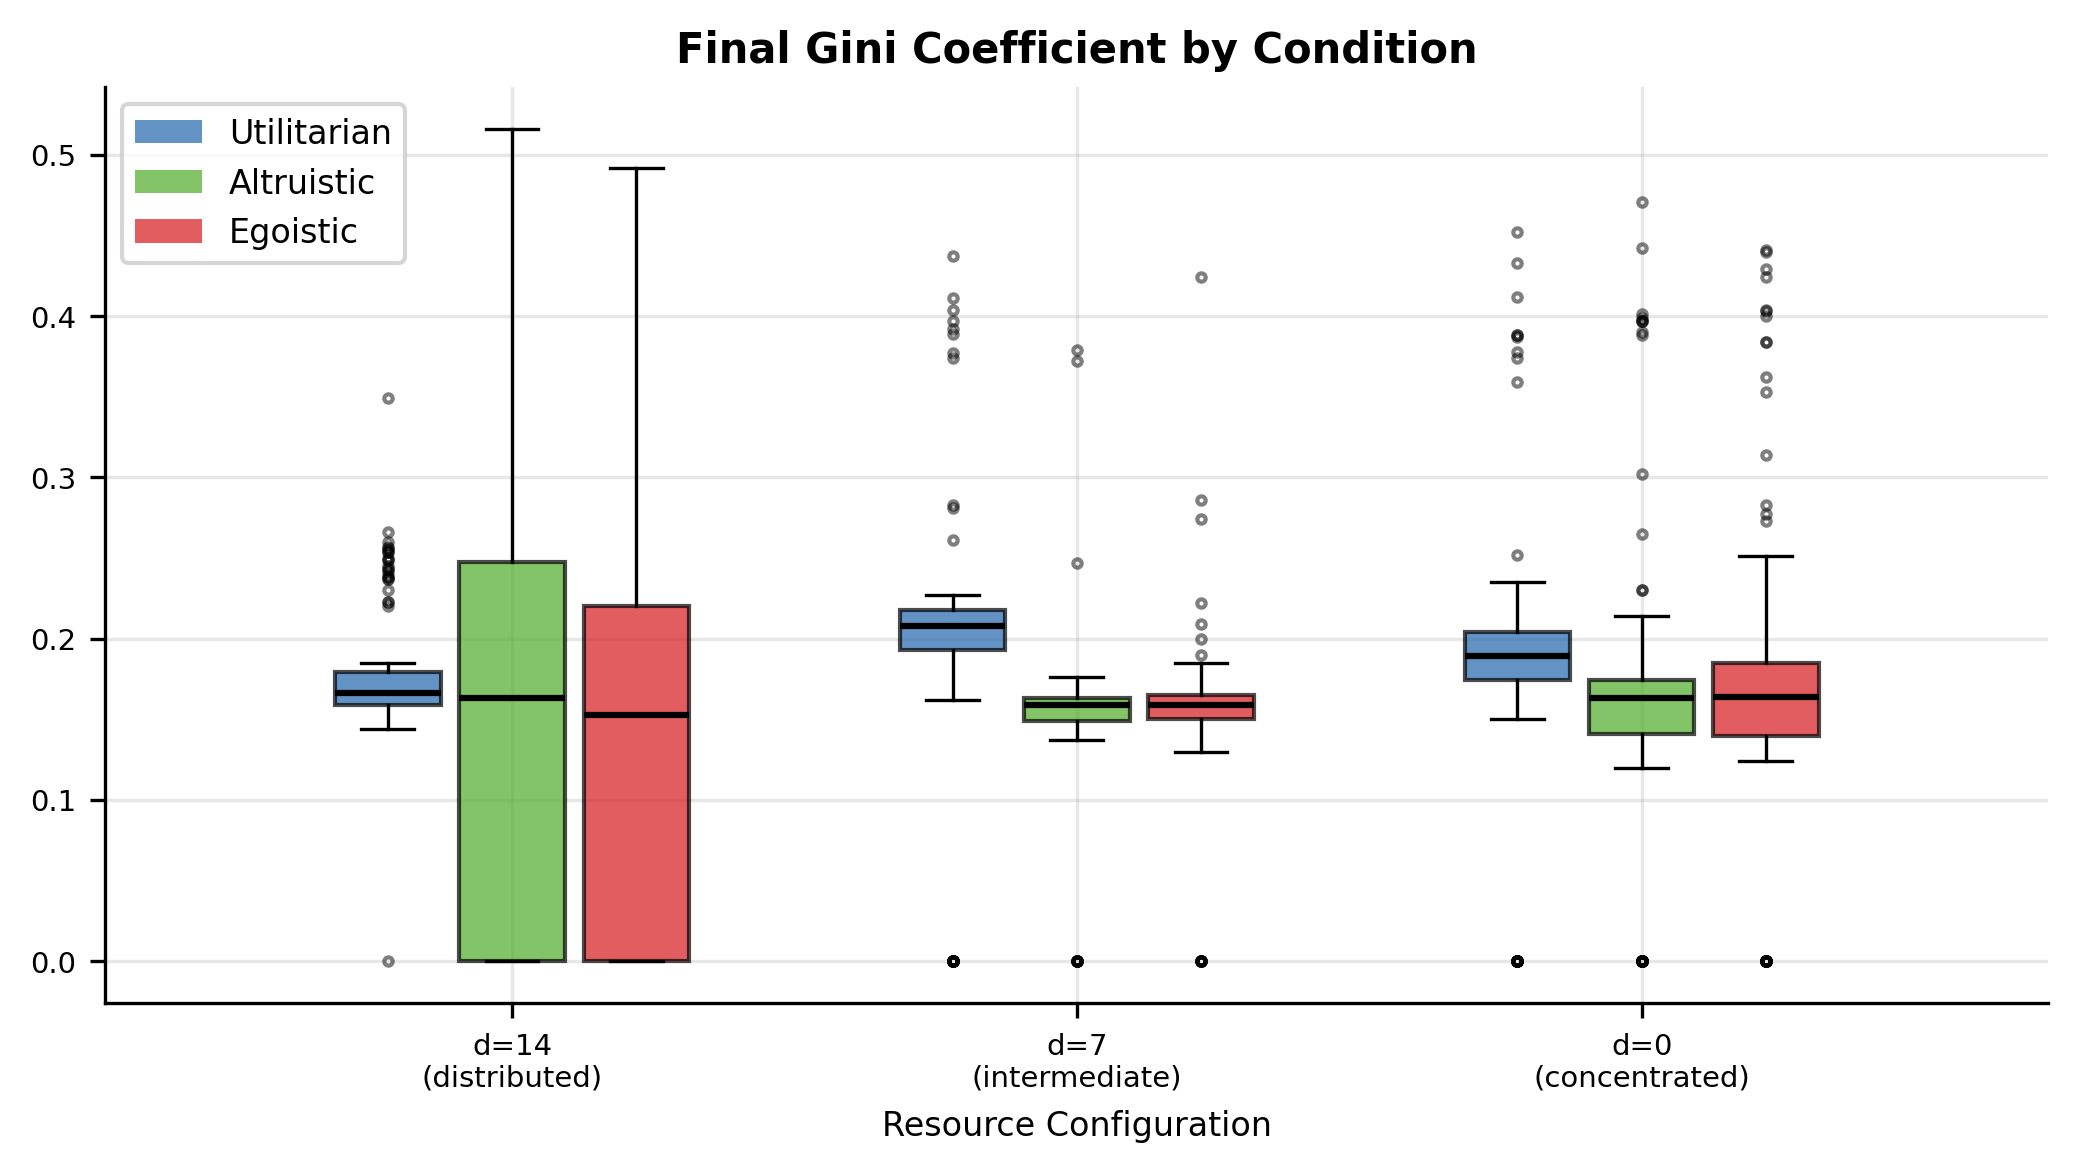
\includegraphics[width=0.85\textwidth]{../../figures/06_boxplot_finalGini.png}
		\par\smallskip
		{\footnotesize\noindent\textit{Note.} Each box spans the IQR across 100 seeds; the horizontal line is the median. Blue = Utilitarian, green = Altruistic, red = Egoistic.}
		\end{figure}

		\begin{figure}[H]
		\caption{Final mean time to live distribution by agent type and resource configuration ($n = 100$ per condition).}
		\label{fig:boxplot-ttl}
		\centering
		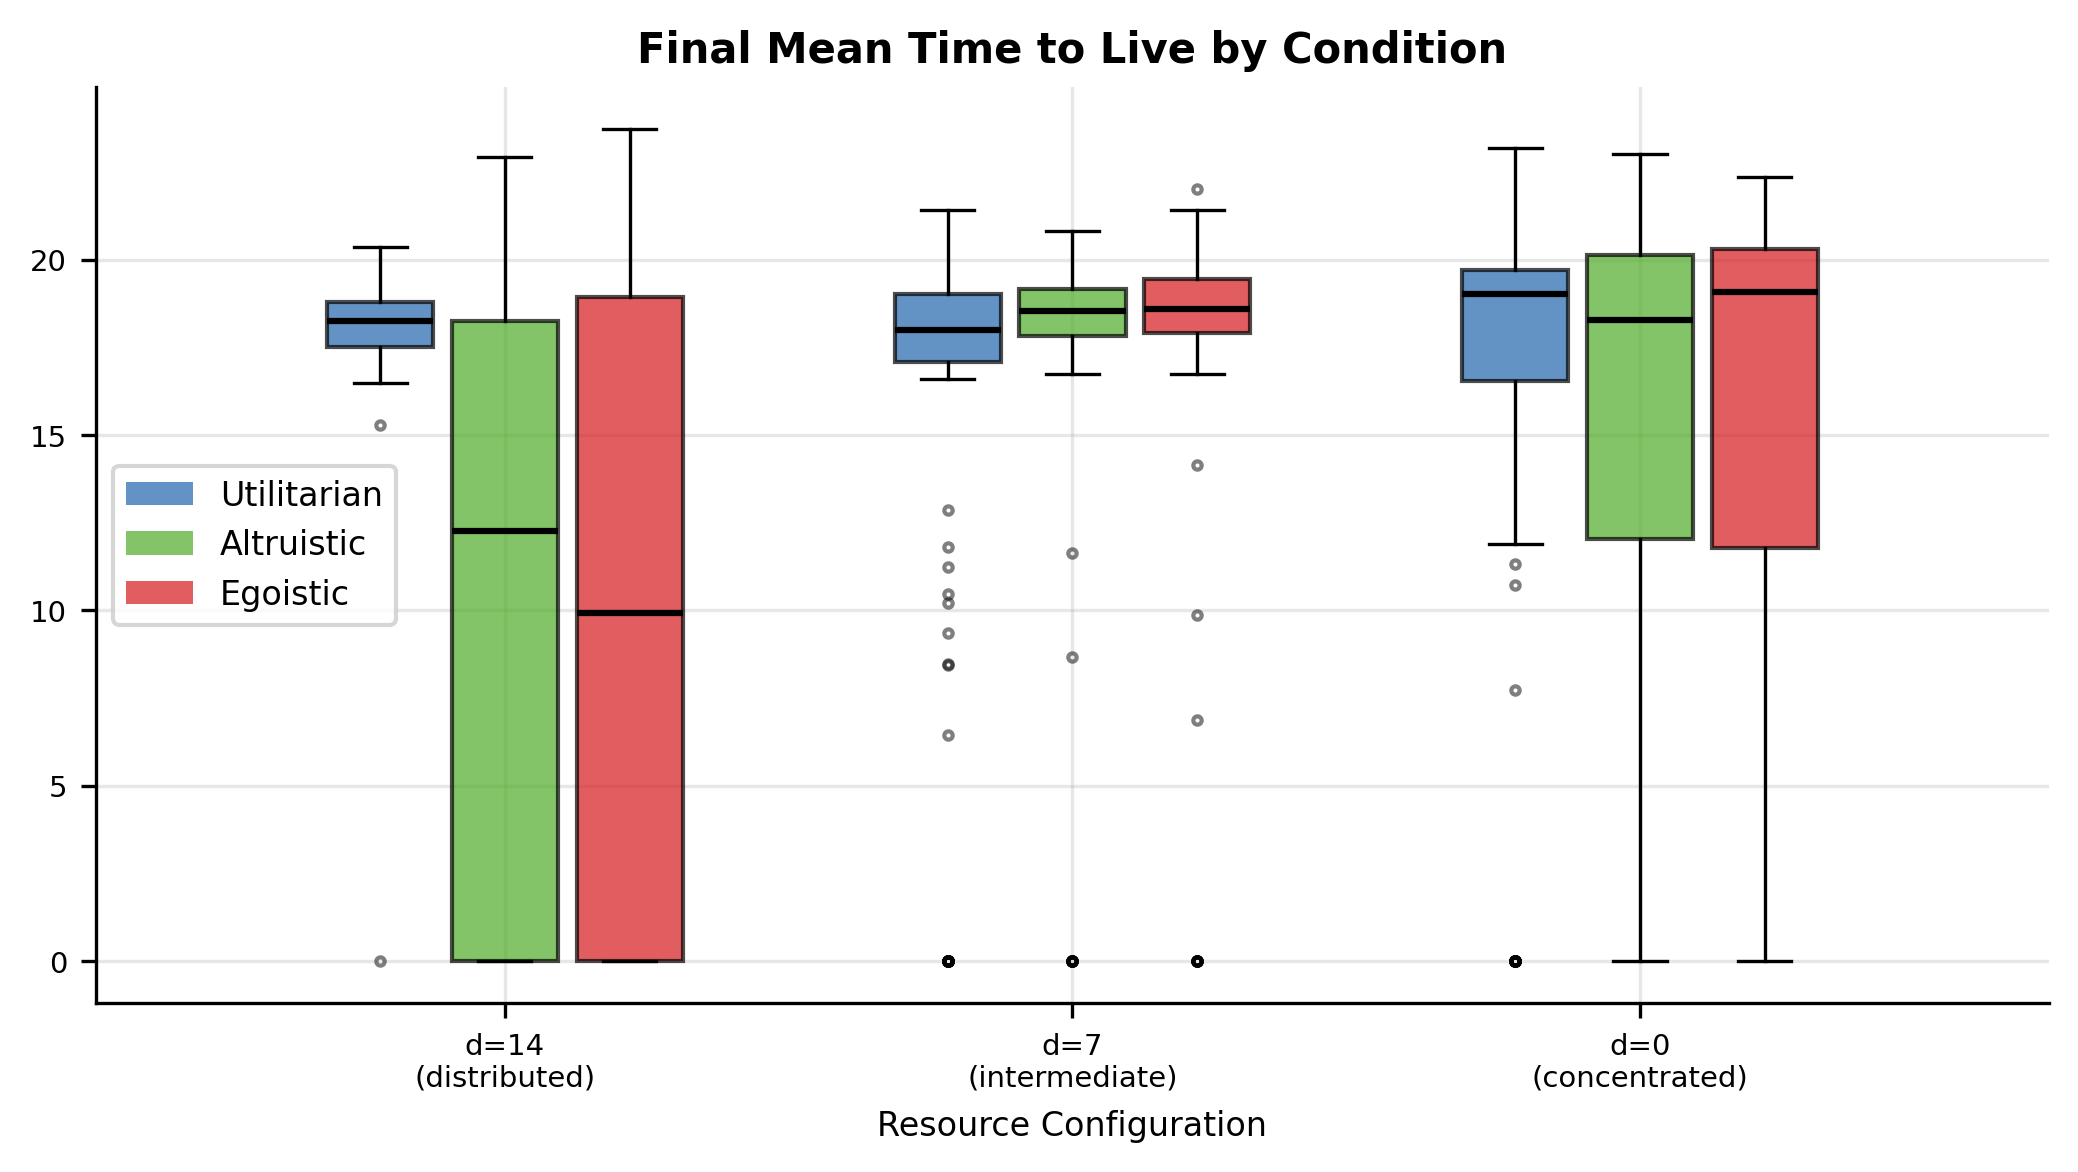
\includegraphics[width=0.85\textwidth]{../../figures/06_boxplot_finalMeanTimeToLive.png}
		\par\smallskip
		{\footnotesize\noindent\textit{Note.} Each box spans the IQR across 100 seeds; the horizontal line is the median. Blue = Utilitarian, green = Altruistic, red = Egoistic. Extinct seeds excluded.}
		\end{figure}

		\begin{figure}[H]
		\caption{Final mean agent wealth distribution by agent type and resource configuration ($n = 100$ per condition).}
		\label{fig:boxplot-meanwealth}
		\centering
		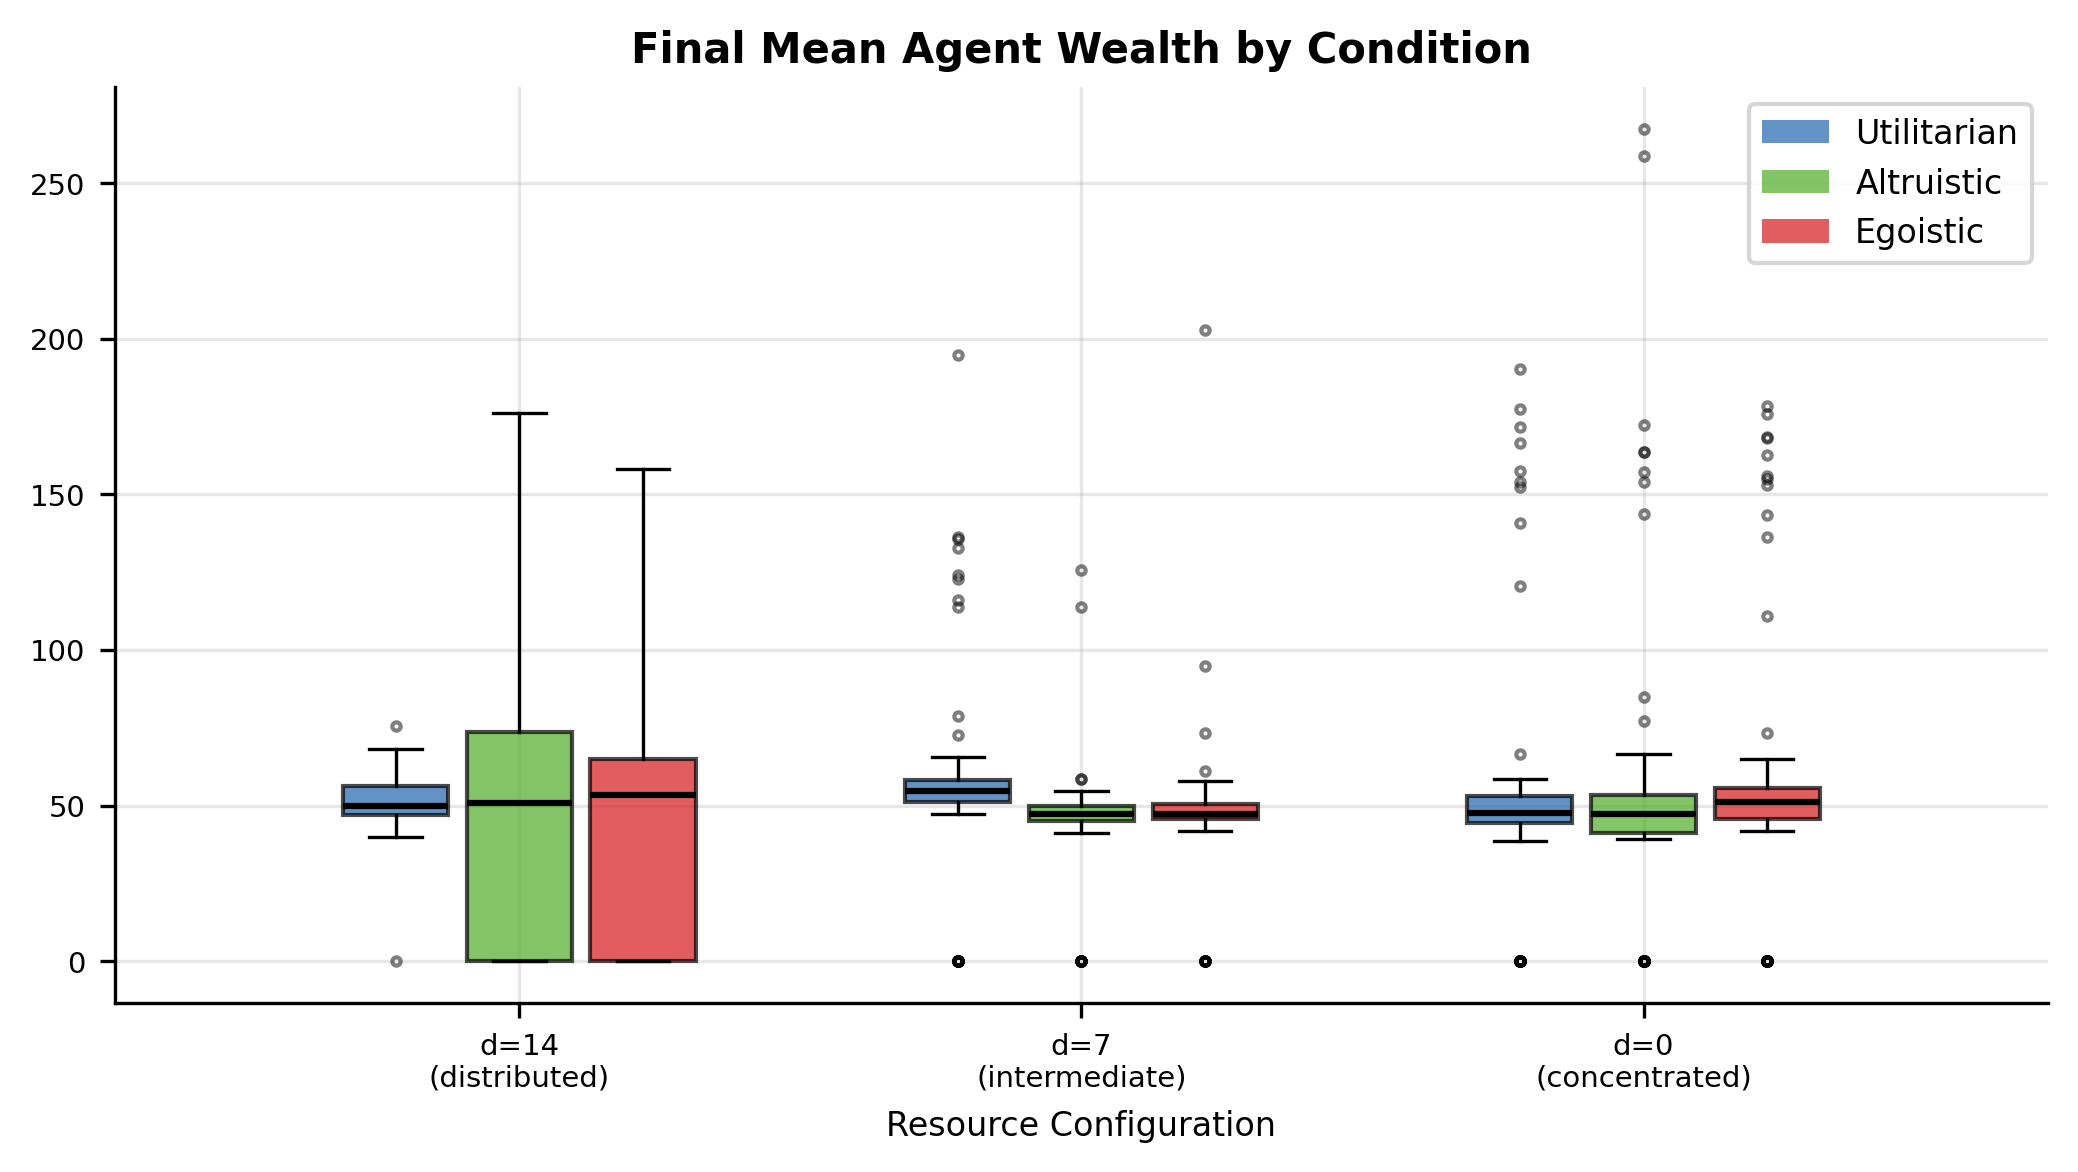
\includegraphics[width=0.85\textwidth]{../../figures/06_boxplot_finalMeanWealth.png}
		\par\smallskip
		{\footnotesize\noindent\textit{Note.} Each box spans the IQR across 100 seeds; the horizontal line is the median. Blue = Utilitarian, green = Altruistic, red = Egoistic. Extinct seeds excluded.}
		\end{figure}

The performance reversal observed at the moderately concentrated ($d = 7$) and concentrated ($d = 0$) configurations constitutes the principal novel finding of this study. Under both configurations, the utilitarian model produced the lowest final population and the highest Gini coefficient of the three models, while egoistic and altruistic models converged to higher performance on both metrics, with pairwise Dunn tests confirming that the utilitarian model differed significantly from at least one non-utilitarian model on every significant metric, while the two non-utilitarian models were statistically indistinguishable from each other on population and Gini coefficient. Effect sizes at the concentrated configuration ($d = 0$) were substantially smaller than at the moderately concentrated configuration ($d = 7$) (population $\eta^2_H = 0.061$ medium vs.\ $0.390$ large; Gini $\eta^2_H = 0.095$ medium vs.\ $0.290$ large), indicating that resource concentration moderates not only the direction but also the magnitude of ethical model differentiation. The reversal suggests that the utilitarian advantage established under distributed conditions may be environment-dependent rather than a fixed property of the decision model.

The reversal is consistent with the competitive restructuring that \citet{Hawick2014} associated with resource concentration. \citet{Hawick2014} found that concentrating resources at opposing peaks fundamentally altered competitive dynamics by drawing all agents toward the same spatial location; in the present study, convergence of the four peaks toward the center similarly funneled the entire population into competition for the same high-value cells.

This spatial convergence exposes a structural property of the selfishness factor formula $h(c) = \phi\, h_{\text{self}} - (1-\phi)\sum_{k \neq \text{self}} h_k$: the penalty a utilitarian agent pays for choosing a cell grows with the value of that cell. A resource-rich cell raises $h_{\text{self}}$ for the scoring agent, but the same abundance that benefits the scoring agent also benefits every neighbor who can reach it, raising each $h_k$ in the sum by a comparable amount. Under the distributed configuration ($d = 14$), agents are spread across the grid and few neighbors compete for any given cell, keeping the sum small relative to $h_{\text{self}}$. Under the concentrated configuration ($d = 0$), the entire population converges on the same location; the sum scales with the number of co-located competitors, and the penalty can exceed $h_{\text{self}}$ entirely, causing the utilitarian agent ($\phi = 0.5$) to score a cell it urgently needs as actively harmful and move away from it. The egoistic agent ($\phi = 1.0$), for which the penalty term reduces to zero regardless of how many neighbors are present, claims those same cells without impediment. Resource concentration thus appears to invert the competitive structure that previously favored the utilitarian model: the better the cell and the more agents competing for it, the more the utilitarian's own scoring rule discourages it from going there.

The near-identical performance of egoistic and altruistic models under concentration reflects the diminishing behavioral differentiation that accompanies extreme resource scarcity. \citet{Fagan2022} found that as resource patches decrease in number, differences between movement strategies narrow because all consumers converge on the same navigational target; at the concentrated configuration ($d = 0$), where the entire resource supply is co-located at the grid center, the distinction between maximizing own welfare ($\phi = 1.0$) and minimizing collective harm ($\phi = 0.0$) becomes inconsequential because both strategies direct agents toward the same cells. The behavioral identities of altruistic and egoistic agents therefore appear to be effectively collapsed by the concentrated environment.

The counterintuitively high Gini coefficient of utilitarian societies at $d = 7$ (0.208 vs.\ 0.159 and 0.159 for altruistic and egoistic) may reflect a scheduling artifact rather than a failure of the collective welfare model. A plausible mechanism is that sequential agent activation creates systematic variation in resource access: agents activated earlier in each timestep encounter central cells with lower projected neighbor densities and claim them first, while later-activated agents find those cells occupied, and this timing advantage may compound over 5,000 timesteps into measurable wealth inequality; \citet{Hawick2014} identified activation order as a general driver of wealth stratification in Sugarscape, where temporal scheduling interacts with spatial competition to determine individual resource outcomes. The utilitarian model's elevated Gini at $d = 7$ is therefore most plausibly attributable to simulation scheduling mechanics rather than to a failure in its collective orientation, though this interpretation would require agent-level instrumentation to verify directly.

The non-zero extinction rates observed at the moderately concentrated ($d = 7$) configuration (14\% utilitarian, 9\% altruistic, 8\% egoistic) and the concentrated ($d = 0$) configuration (14\%, 20\%, 17\%, respectively) with $n = 100$ seeds indicate that the zero extinction apparent in the prior $n = 50$ run was an artifact of insufficient sample size. Despite the non-zero rates at the moderately concentrated ($d = 7$) and concentrated ($d = 0$) configurations, the chi-square tests confirmed no significant between-model difference in extinction frequency at either configuration ($p = 0.328$ and $p = 0.528$, respectively), suggesting a shared stochastic survival threshold across ethical orientations under moderate to high resource concentration rather than model-specific vulnerability.

The moderately concentrated ($d = 7$) and concentrated ($d = 0$) results suggest that the utilitarian advantage at the distributed configuration ($d = 14$) may not generalize across resource environments: under both the moderately concentrated ($d = 7$) and concentrated ($d = 0$) configurations, the utilitarian model produced the lowest final population and the highest Gini coefficient, while the two non-utilitarian models performed equivalently on both metrics. The convergence of altruistic and egoistic outcomes, the scheduling-driven Gini paradox, and the reduction in effect sizes from the moderately concentrated ($d = 7$) to the concentrated ($d = 0$) configuration together suggest that resource geography may not merely scale existing performance differences but may restructure the competitive logic through which ethical orientations produce societal outcomes, with differentiation strength peaking at the moderately concentrated configuration before diminishing under the concentrated configuration.

		\subsection{Objective 2: Effect Sizes Across Resource Configurations}

Figures~\ref{fig:effectsize-population}--\ref{fig:effectsize-meanwealth} plot $\eta^2_H$ as a function of peak distance $d$ for each metric. Table~\ref{table:effect-sizes} reports the numerical values; the full Kruskal-Wallis test statistics are in Table~\ref{table:app-kw}. Effect size varied across configurations for all five metrics, though the magnitude and direction of variation differed by metric.

		\begin{figure}[H]
		\caption{$\eta^2_H$ effect size as a function of peak distance $d$: final population (Objective~2).}
		\label{fig:effectsize-population}
		\centering
		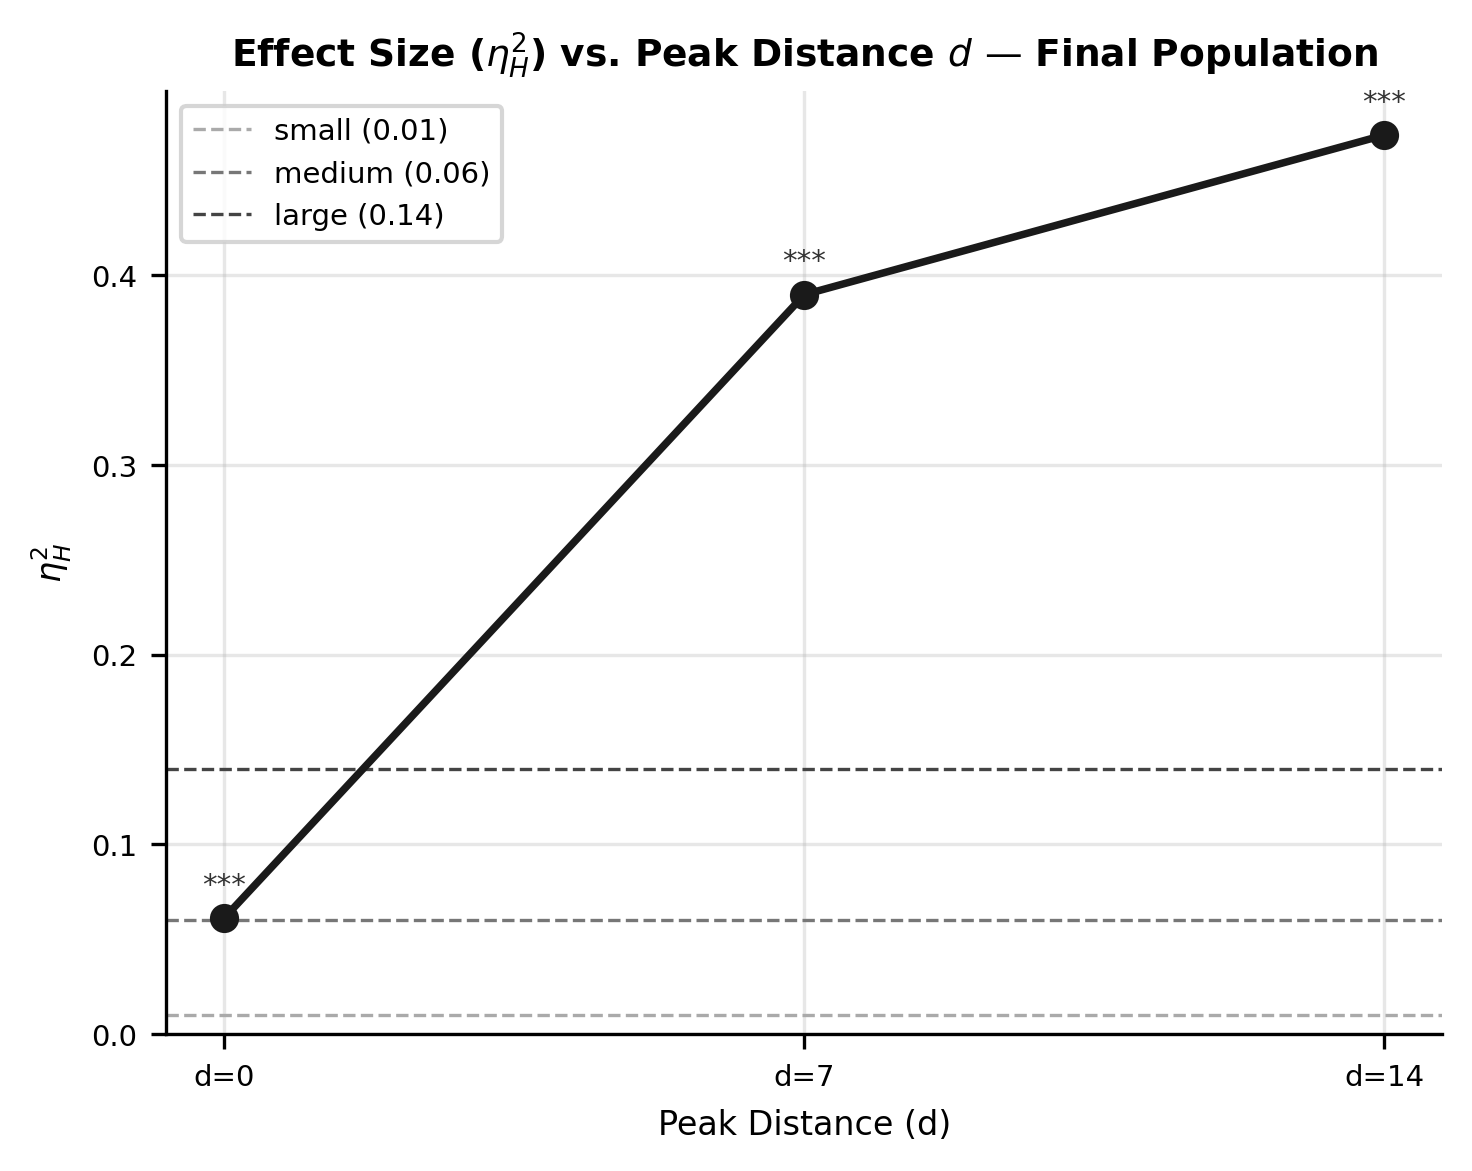
\includegraphics[width=0.65\textwidth]{../../figures/08_effectSize_finalPopulation.png}
		\par\smallskip
		{\footnotesize\noindent\textit{Note.} Dashed lines mark small (0.01), medium (0.06), and large (0.14) thresholds per \citet{Tomczak2014}. Significance markers from the Kruskal-Wallis omnibus test.}
		\end{figure}

		\begin{figure}[H]
		\caption{$\eta^2_H$ effect size as a function of peak distance $d$: final societal wealth (Objective~2).}
		\label{fig:effectsize-wealth}
		\centering
		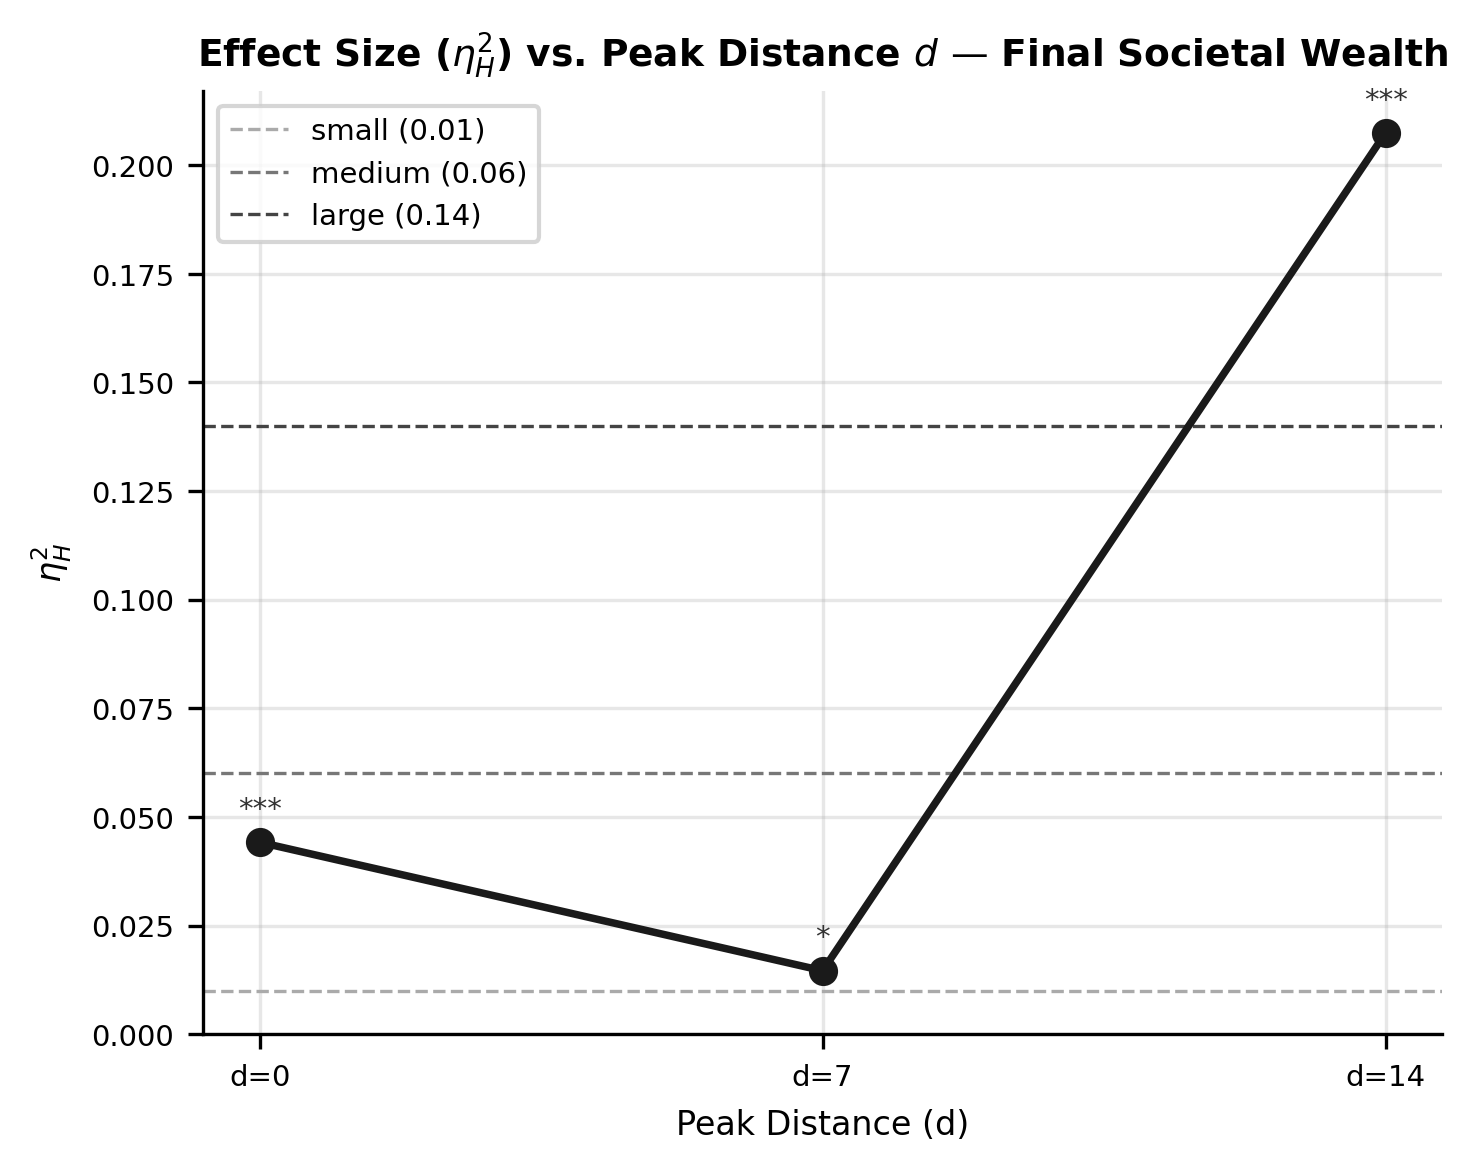
\includegraphics[width=0.65\textwidth]{../../figures/08_effectSize_finalSocietalWealth.png}
		\par\smallskip
		{\footnotesize\noindent\textit{Note.} Dashed lines mark small (0.01), medium (0.06), and large (0.14) thresholds per \citet{Tomczak2014}. Significance markers from the Kruskal-Wallis omnibus test.}
		\end{figure}

		\begin{figure}[H]
		\caption{$\eta^2_H$ effect size as a function of peak distance $d$: Gini coefficient (Objective~2).}
		\label{fig:effectsize-gini}
		\centering
		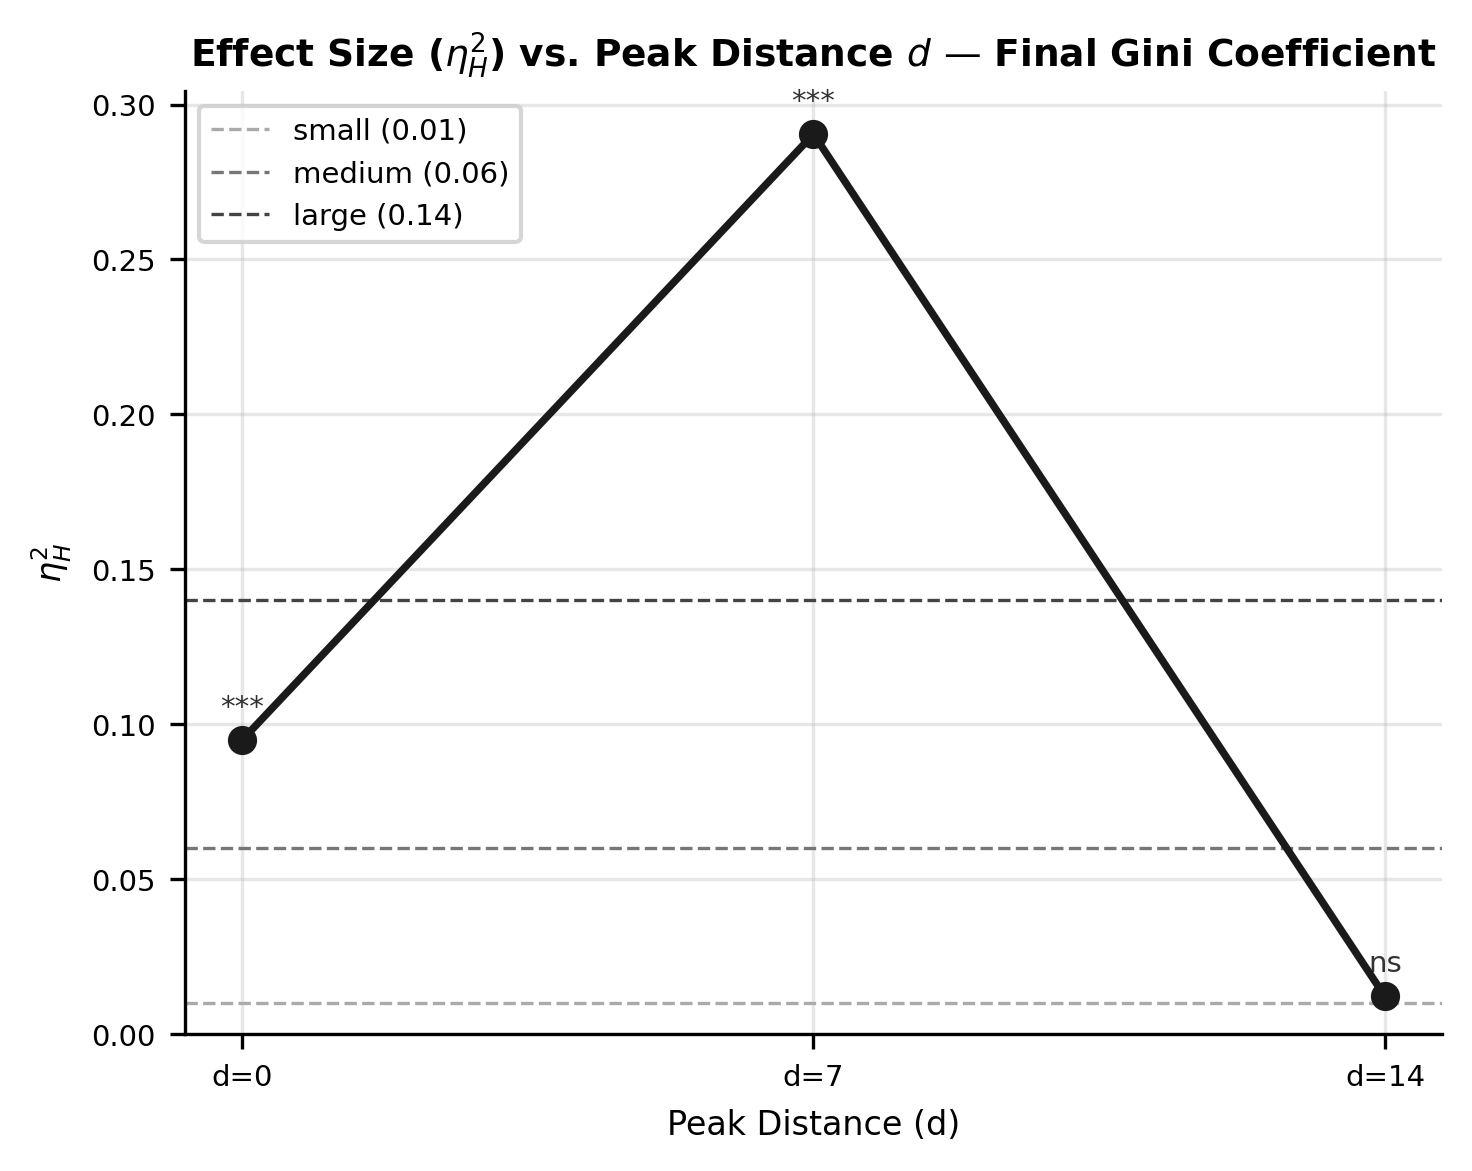
\includegraphics[width=0.65\textwidth]{../../figures/08_effectSize_finalGini.png}
		\par\smallskip
		{\footnotesize\noindent\textit{Note.} Dashed lines mark small (0.01), medium (0.06), and large (0.14) thresholds per \citet{Tomczak2014}. Significance markers from the Kruskal-Wallis omnibus test.}
		\end{figure}

		\begin{figure}[H]
		\caption{$\eta^2_H$ effect size as a function of peak distance $d$: mean time to live (Objective~2).}
		\label{fig:effectsize-ttl}
		\centering
		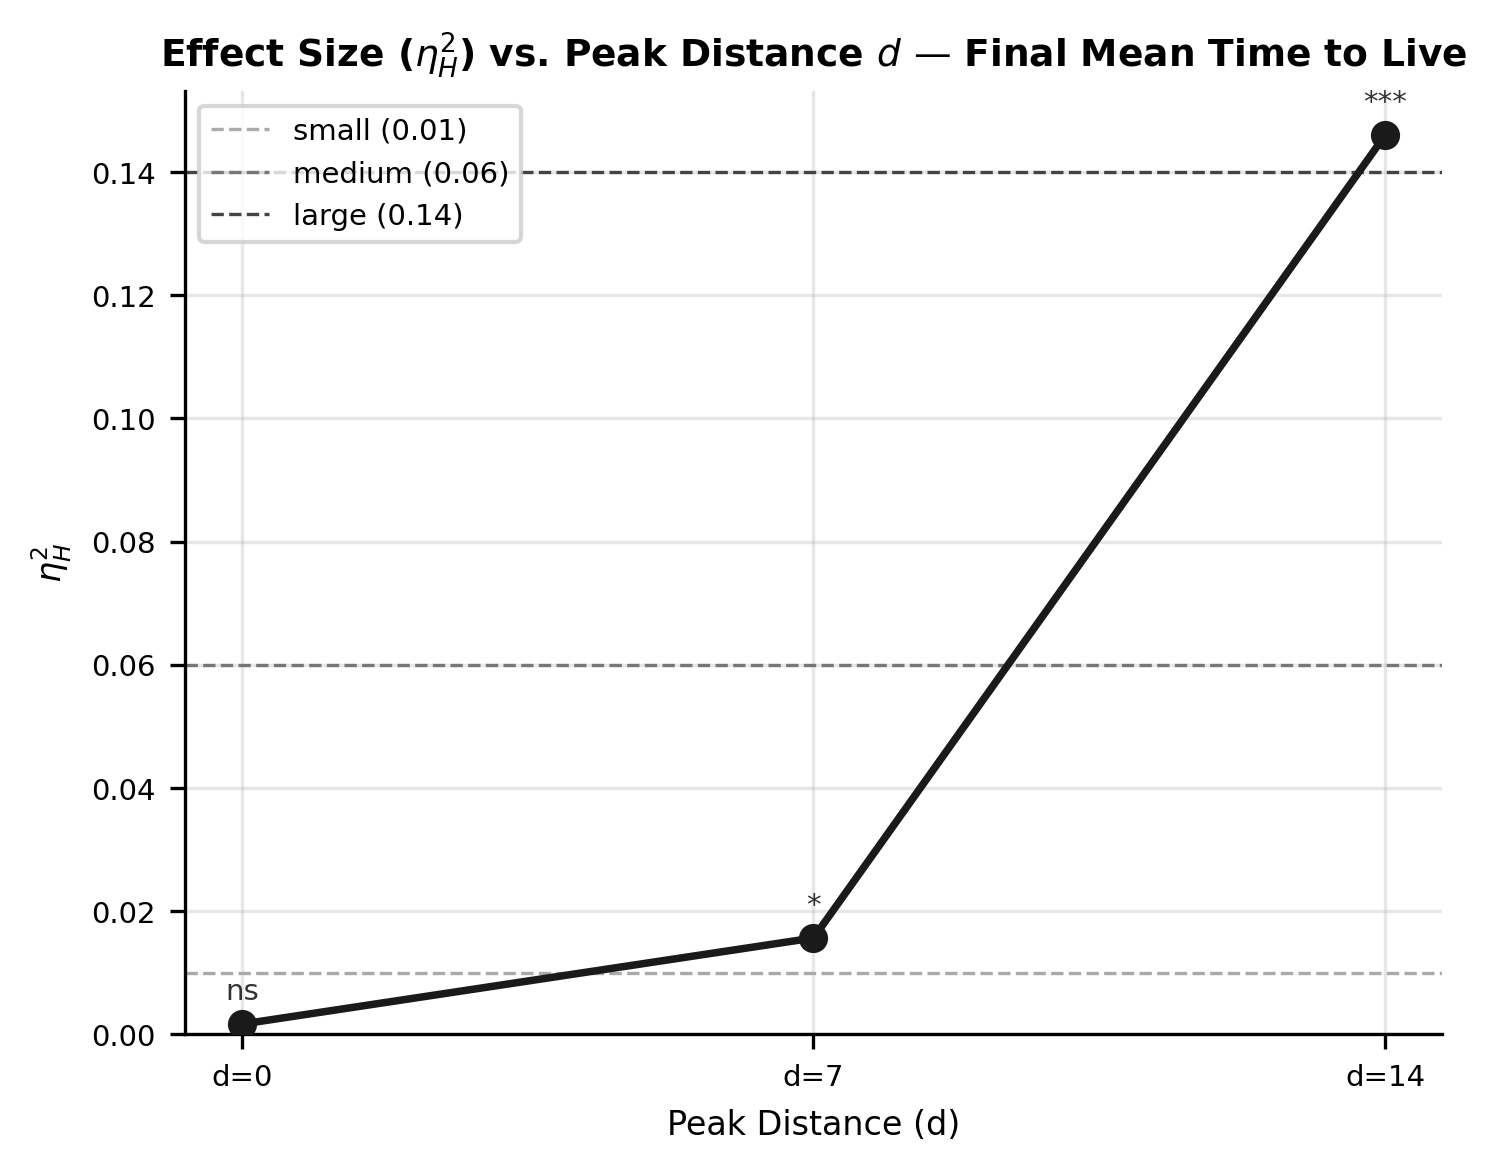
\includegraphics[width=0.65\textwidth]{../../figures/08_effectSize_finalMeanTimeToLive.png}
		\par\smallskip
		{\footnotesize\noindent\textit{Note.} Dashed lines mark small (0.01), medium (0.06), and large (0.14) thresholds per \citet{Tomczak2014}. Significance markers from the Kruskal-Wallis omnibus test.}
		\end{figure}

		\begin{figure}[H]
		\caption{$\eta^2_H$ effect size as a function of peak distance $d$: mean agent wealth (Objective~2).}
		\label{fig:effectsize-meanwealth}
		\centering
		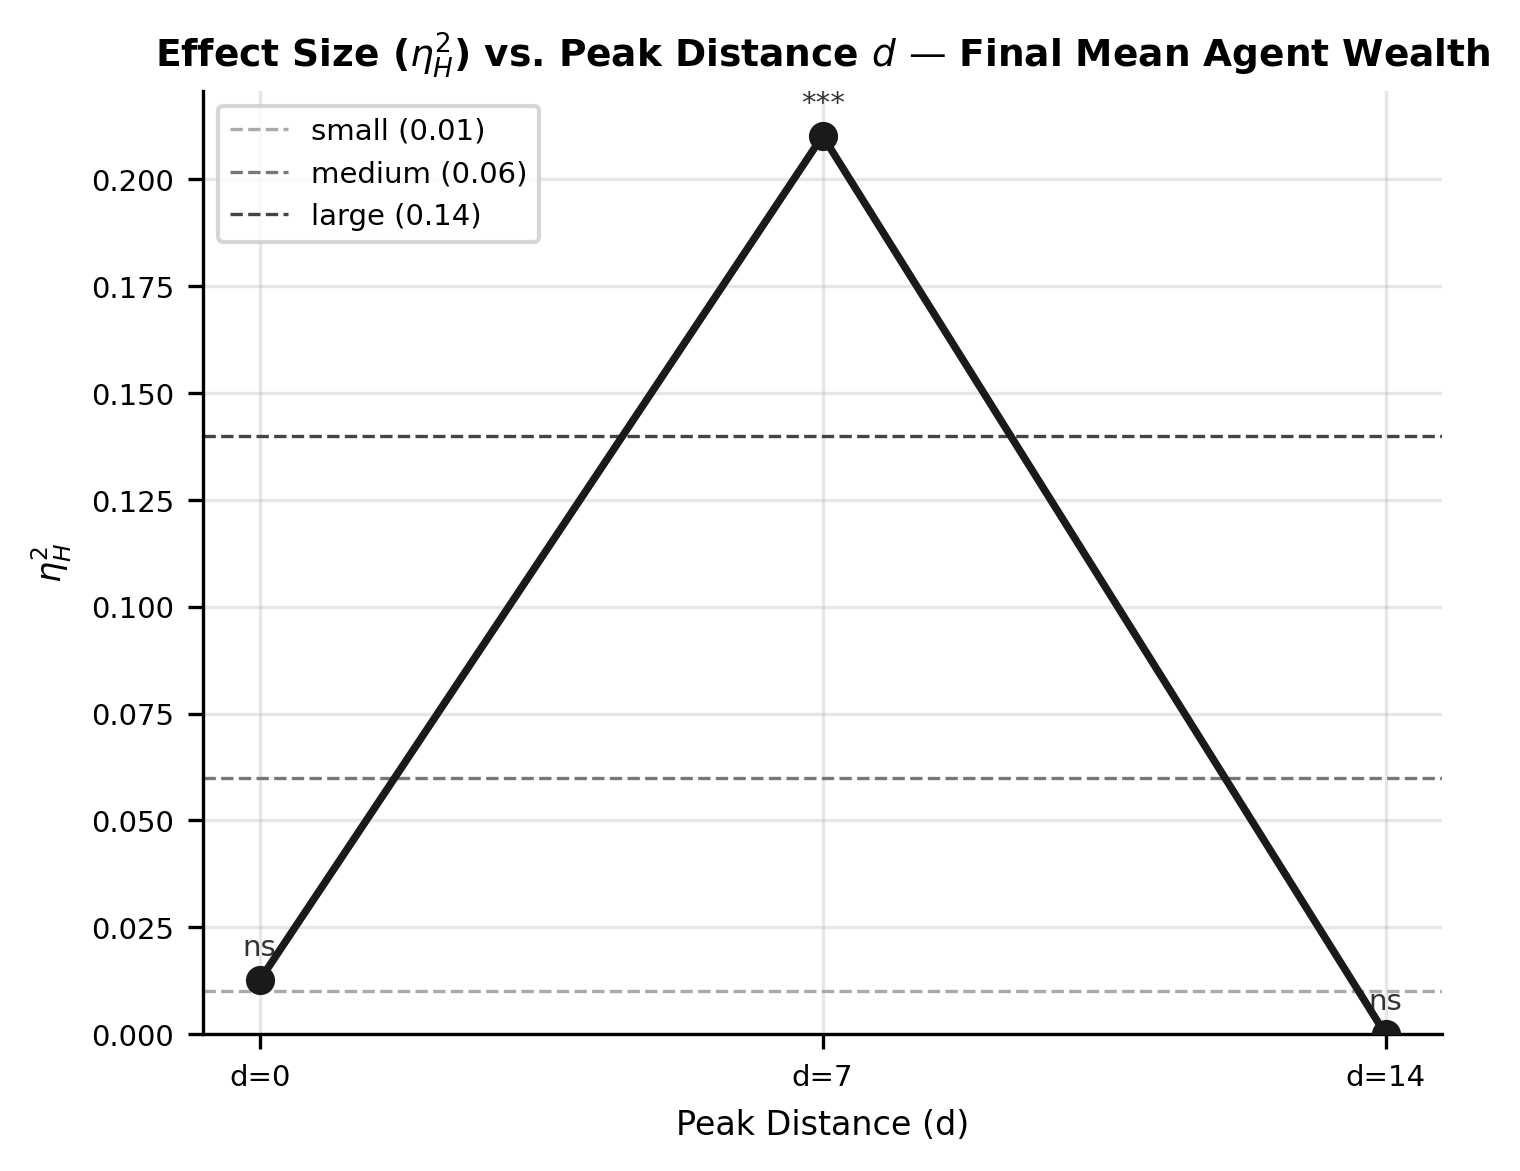
\includegraphics[width=0.65\textwidth]{../../figures/08_effectSize_finalMeanWealth.png}
		\par\smallskip
		{\footnotesize\noindent\textit{Note.} Dashed lines mark small (0.01), medium (0.06), and large (0.14) thresholds per \citet{Tomczak2014}. Significance markers from the Kruskal-Wallis omnibus test.}
		\end{figure}

For final population, $\eta^2_H$ decreased monotonically from $d = 14$ (0.474, large) to $d = 7$ (0.390, large) to $d = 0$ (0.061, medium). For final societal wealth, $\eta^2_H$ was largest at $d = 14$ (0.207, large), then dropped sharply at $d = 7$ (0.015, small) and $d = 0$ (0.044, small), a non-monotonic pattern driven by the extinction-based contrast at $d = 14$. For Gini coefficient, $\eta^2_H$ was largest at $d = 7$ (0.290, large), intermediate at $d = 0$ (0.095, medium), and small but not significant at $d = 14$ (0.012, $p = 0.060$, ns). Mean time to live yielded a large effect at $d = 14$ ($\eta^2_H = 0.146$, $p < 0.001$) reflecting extinction-driven distributional differences, a small effect at $d = 7$ ($\eta^2_H = 0.016$, $p = 0.036$), and was negligible at $d = 0$ (0.002). Mean agent wealth was not significant at $d = 14$ (0.000) or $d = 0$ (0.013, $p = 0.057$), but yielded a large effect at $d = 7$ ($\eta^2_H = 0.210$, $p < 0.001$). $H_{0,4}$ was rejected for final population, societal wealth, Gini coefficient, mean time to live, and mean agent wealth.

		\begin{table}[H]
		\vspace{2ex}
		\centering
		\caption{$\eta^2_H$ Effect Size by Outcome Metric and Resource Configuration}
		\label{table:effect-sizes}
		\footnotesize
		\renewcommand{\arraystretch}{1.3}
		\begin{tabular}{
			>{\raggedright\arraybackslash}p{3.8cm}
			r r r
		}
		\hline\hline
		\textbf{Metric} & $d = 14$ & $d = 7$ & $d = 0$ \\
		\hline
		Final Population       & 0.474 & 0.390 & 0.061 \\
		Final Societal Wealth  & 0.207 & 0.015$^{*}$ & 0.044 \\
		Final Gini Coefficient & 0.012$^{ns}$ & 0.290 & 0.095 \\
		Mean TTL               & 0.146 & 0.016$^{*}$ & 0.002 \\
		Mean Agent Wealth      & 0.000$^{ns}$ & 0.210 & 0.013$^{ns}$ \\
		\hline
		\end{tabular}
		\par\smallskip
		{\footnotesize\noindent\textit{Note.} Thresholds per \citet{Tomczak2014}: negligible $< 0.01$, small $0.01$--$0.06$, medium $0.06$--$0.14$, large $\geq 0.14$. Superscript $ns$ = Kruskal-Wallis $p \geq 0.05$; $^{*}p < 0.05$; $^{**}p < 0.01$; all other entries $p < 0.001$. Complete KW statistics including $H$, $p$, and significance codes in Table~\ref{table:app-kw}.}
		\end{table}

Resource geography appeared to moderate the practical magnitude of ethical model differences across all outcome metrics, providing evidence against $H_{0,4}$. As reported in Table~\ref{table:effect-sizes} and visualized in Figures~\ref{fig:effectsize-population}--\ref{fig:effectsize-meanwealth}, $\eta^2_H$ varied substantially across configurations for final population, societal wealth, and Gini coefficient, and varied selectively for mean time to live, which showed a small but significant effect at the moderately concentrated configuration ($d = 7$, $\eta^2_H = 0.016$) while remaining negligible at the concentrated configuration ($d = 0$). The magnitude of ethical differentiation therefore appears not to be a fixed property of the decision models but may depend on the spatial structure of the resource environment.

The effect size pattern for final population reflects qualitatively different differentiation mechanisms at each configuration. At $d = 14$, the population effect ($\eta^2_H = 0.474$) is largely driven by the sharp binary contrast between models with near-zero extinction (utilitarian 1\%) and models with high extinction rates (altruistic 44\%, egoistic 47\%); this extinction-driven separation produces the largest rank-based effect despite substantial distributional overlap among surviving seeds. At the moderately concentrated configuration ($d = 7$), where extinction is less asymmetric across models (8--14\%), consistently distinct population levels are produced across surviving seeds, yielding a large but somewhat smaller effect ($\eta^2_H = 0.390$); at the concentrated configuration ($d = 0$), absolute between-model differences are smaller and the three models' distributions overlap more substantially, reducing the effect to medium ($\eta^2_H = 0.061$). The Gini effect, by contrast, is small at the distributed configuration ($d = 14$) (where the bimodal structure driven by extinction distorts the inequality metric) and peaks at the moderately concentrated configuration ($d = 7$, $\eta^2_H = 0.290$), where all models produce stable terminal societies with consistently distinct inequality levels across seeds.

The societal wealth effect size pattern ($\eta^2_H = 0.207$ at the distributed ($d = 14$), dropping to $0.015$ at the moderately concentrated ($d = 7$) and $0.044$ at the concentrated ($d = 0$)) reflects a different mechanism than the other metrics. The large effect at the distributed configuration ($d = 14$) is predominantly extinction-driven: the 44\% and 47\% extinction rates in altruistic and egoistic conditions produce many near-zero final wealth values, while utilitarian societies consistently accumulate high wealth, generating a large rank-based separation. At the moderately concentrated ($d = 7$) and concentrated ($d = 0$) configurations, where all models produce surviving societies with relatively similar per-agent resource acquisition, the between-model wealth contrast collapses to small effects despite the significant omnibus tests. Mean agent wealth at the moderately concentrated configuration ($d = 7$, $\eta^2_H = 0.210$, large) shows that the utilitarian model supports higher per-agent wealth than altruistic and egoistic models, suggesting that the utilitarian population's lower headcount concentrates resources among the surviving agents rather than distributing them uniformly. This pattern extends the finding of \citet{Hawick2014} that resource geography interacts with agent decision logic to produce model-dependent resource outcomes, while demonstrating that the mechanism driving wealth differentiation shifts from extinction-based at the distributed configuration ($d = 14$) to per-agent acquisition differences at the moderately concentrated configuration ($d = 7$).

Mean time to live presented a complex pattern across configurations. The large effect at the distributed configuration ($d = 14$, $\eta^2_H = 0.146$, $p < 0.001$) is predominantly an artifact of the large extinction-rate differences: extinct seeds contribute near-zero TTL values that depress the altruistic and egoistic medians substantially below the utilitarian median, and the effect disappears when surviving seeds alone are considered. At the moderately concentrated configuration ($d = 7$), a small but significant effect remained ($\eta^2_H = 0.016$, $p = 0.036$), with egoistic agents maintaining the highest median TTL (18.585) and utilitarian agents the lowest (18.005); pairwise Dunn tests identified a significant difference only between egoistic and utilitarian models ($p = 0.048$), while altruistic and utilitarian did not differ significantly ($p = 0.138$). This is consistent with the interpretation that the utilitarian model's neighbor-discounting penalty modestly reduces individual agent longevity at the moderately concentrated configuration. At the concentrated configuration ($d = 0$), the TTL effect was negligible ($\eta^2_H = 0.002$, $p = 0.288$), suggesting that the ethical model's influence on individual longevity is specific to the moderately concentrated competitive regime. The small effect size at the moderately concentrated configuration ($d = 7$) and the absence of this pattern at the concentrated configuration ($d = 0$) counsel caution in treating TTL differentiation as a robust substantive finding beyond the specific interplay of moderate density and scheduling mechanics.

Effect size analysis suggests that the sensitivity of societal outcomes to ethical orientation may depend on the resource environment. Population and societal wealth effects are largest at the distributed configuration ($d = 14$) but primarily reflect extinction-rate differences rather than between-model contrasts among surviving societies. Gini and mean agent wealth effects peak at the moderately concentrated configuration ($d = 7$), where stable competing societies expose the clearest behavioral differentiation. At the concentrated configuration ($d = 0$), all effects are reduced, consistent with the narrowing of behavioral distinction predicted by patch-depletion models. The selective emergence of mean time to live differentiation at the moderately concentrated configuration ($d = 7$) and its absence at the concentrated configuration ($d = 0$) further suggest that the conditions under which ethical orientation affects individual welfare are narrower than those under which it affects collective outcomes, and that resource geography may selectively activate or suppress metric-specific pathways through which decision logic shapes population dynamics.

		\subsection{Objective 3: Best Resource Configuration for Comparing Ethical Decision Models}

The effect size analysis in Objective~2 identified the moderately concentrated configuration ($d = 7$) as the resource layout that produces the clearest behavioral differentiation between ethical decision models. To understand why, it helps to separate two different ways a configuration can produce a large effect size: survival contrast and behavioral contrast.

At the distributed configuration ($d = 14$), the largest effects for population ($\eta^2_H = 0.474$) and societal wealth ($\eta^2_H = 0.207$) are driven by an extreme survival split: utilitarian societies almost never go extinct (1\% of runs), while altruistic and egoistic societies do so frequently (44\% and 47\%). That gap is real, but it tells us mainly which model survives, not how surviving agents actually behave differently from one another. It is like comparing exam scores across students where one group finished the test and another left halfway through; the difference is large, but it reflects who stayed in the room more than what each person knew.

At the moderately concentrated configuration ($d = 7$), all three models produce surviving societies across most seeds (extinction rates of 8--14\%), so every comparison is between societies that made it to the end. Three metrics show large, clean effects at this configuration: final population ($\eta^2_H = 0.390$), Gini coefficient ($\eta^2_H = 0.290$), and mean agent wealth ($\eta^2_H = 0.210$). These effects reflect persistent behavioral differences (how many agents each model supports, how evenly resources are distributed, and how wealthy individual agents become) rather than a survival threshold. The direction of those effects also reverses from the distributed configuration ($d = 14$): at the moderately concentrated configuration ($d = 7$), altruistic and egoistic models outperform the utilitarian on population and Gini, which would be invisible if only the distributed configuration were tested.

At the concentrated configuration ($d = 0$), all effects shrink (population $\eta^2_H = 0.061$, Gini $\eta^2_H = 0.095$, societal wealth $\eta^2_H = 0.044$), consistent with the prediction that behavioral strategies converge when all agents are funneled to the same location and differences in decision logic no longer translate into differences in navigational choice.

The moderately concentrated configuration ($d = 7$) therefore appears to be the resource layout best suited to comparing ethical decision models. It avoids the extinction-driven inflation of the distributed configuration ($d = 14$), which can make differences look large for the wrong reason, and it avoids the behavioral collapse of the concentrated configuration ($d = 0$), which suppresses real differences. Researchers who wish to study how ethical orientation shapes the way agents live, rather than just whether they survive, should use a resource layout that concentrates competition enough to expose behavioral distinctions without funneling the entire population to a single point.

		\subsection{Objective 4: Runtime Benchmarks for the Digital Terrarium}

Table~\ref{table:exec-time} reports the mean and standard deviation of wall-clock execution time per condition. Execution times were comparable across ethical models within each configuration, consistent with the structurally identical felicific calculus procedure used by all three models ($\phi$ is the only parameter that varies). Differences across configurations primarily reflected differences in sustained population size.

		\begin{table}[H]
		\vspace{2ex}
		\centering
		\caption{Wall-Clock Execution Time per Simulation Run by Condition ($n = 100$ per condition)}
		\label{table:exec-time}
		\footnotesize
		\renewcommand{\arraystretch}{1.3}
		\begin{tabular}{l l r r r r}
		\hline\hline
		\textbf{Config} & \textbf{Model} & \textbf{Mean (s)} & \textbf{SD (s)} & \textbf{Median (s)} & \textbf{IQR (s)} \\
		\hline
		\multirow{3}{*}{$d = 14$ (distributed)}
		  & Utilitarian & 3332.0 & 1434.1 & 3890.7 & 2366.4 \\
		  & Altruistic  & 1166.3 & 1306.1 &  671.5 & 2330.5 \\
		  & Egoistic    & 1020.4 & 1187.4 &  765.6 & 1810.6 \\
		\hline
		\multirow{3}{*}{$d = 7$ (moderately concentrated)}
		  & Utilitarian &  579.6 & 289.7 &  659.1 & 111.6 \\
		  & Altruistic  & 1746.9 & 616.7 & 1928.5 & 300.5 \\
		  & Egoistic    & 1684.8 & 607.8 & 1876.4 & 306.5 \\
		\hline
		\multirow{3}{*}{$d = 0$ (concentrated)}
		  & Utilitarian &  280.6 & 133.7 &  325.0 &  47.4 \\
		  & Altruistic  &  634.3 & 397.3 &  808.1 & 748.7 \\
		  & Egoistic    &  667.6 & 414.8 &  806.9 & 736.9 \\
		\hline
		\end{tabular}
		\par\smallskip
		{\footnotesize\noindent\textit{Note.} Values in seconds. Statistics computed across $n = 100$ seeds per condition. Large IQRs at $d = 14$ Altruistic (2,330.5 s) and Egoistic (1,810.6 s) and at $d = 0$ reflect the bimodal distribution of run durations driven by early-terminating extinct seeds alongside full 5,000-timestep runs.}
		\end{table}

The present study provides wall-clock execution time benchmarks for the Sugarscape Digital Terrarium across all nine experimental conditions, supplementing the computational reference absent from the original study by \citet{KremerHerman2024}. As shown in Table~\ref{table:exec-time}, execution times within each configuration were comparable across ethical models, consistent with the structurally identical felicific calculus procedure used by all three models; differences across configurations reflect differences in sustained population size. The utilitarian model at $d = 14$ had a substantially higher median execution time (3,890.7 s) than altruistic (671.5 s) and egoistic (765.6 s) at the same configuration, because utilitarian agents rarely go extinct (1\% of runs) and therefore almost always complete the full 5,000-timestep budget while altruistic and egoistic agents go extinct in 44\% and 47\% of runs, producing many early-terminating seeds. The same extinction-driven bimodality explains the large IQRs for altruistic (2,330.5 s) and egoistic (1,810.6 s) at $d = 14$, and for altruistic (748.7 s) and egoistic (736.9 s) at $d = 0$. The benchmark confirms that the Digital Terrarium's computational cost scales with population size rather than with the ethical decision model employed.

Researchers planning replications or parameter sweeps of the Digital Terrarium should account for configuration-driven population differences and extinction-driven bimodality when estimating run time, as the dominant determinant of execution cost is the number of agents surviving to complete the full timestep budget rather than the mathematical structure of the felicific calculus itself.

		\section{SUMMARY AND CONCLUSION}

		\subsection{Summary}

This study examined the effects of resource concentration on the societal outcomes of ethical decision models in the Sugarscape Digital Terrarium simulation \citep{KremerHerman2024}. The general objective was to determine whether the comparative advantage of utilitarian agents over altruistic and egoistic agents, established by \citet{KremerHerman2024} under a fixed distributed resource environment, was maintained, strengthened, or weakened as resource peaks converged toward the grid center. Three ethical decision models were compared across three resource configurations defined by the radial peak distance $d$: distributed ($d = 14$), moderately concentrated ($d = 7$), and concentrated ($d = 0$). Each of the nine experimental conditions was run across 100 independent random seeds for 5,000 timesteps. Five continuous outcome metrics were analyzed using Kruskal-Wallis tests: final population, societal wealth, Gini coefficient of wealth inequality, mean time to live, and mean agent wealth. Extinction rate was analyzed separately using Pearson chi-square tests at each configuration.

Under the distributed configuration ($d = 14$), the utilitarian model replicated the findings of \citet{KremerHerman2024}. It achieved the highest median final population (1,425.5; IQR = 178.3) and went extinct in only 1\% of the 100 observed seeds, while altruistic and egoistic models went extinct in 44\% and 47\% of seeds, respectively. The Kruskal-Wallis test confirmed large, statistically significant differences in final population ($H = 142.774$, $p < 0.001$, $\eta^2_H = 0.474$), societal wealth ($H = 63.611$, $p < 0.001$, $\eta^2_H = 0.207$), and mean time to live ($H = 45.350$, $p < 0.001$, $\eta^2_H = 0.146$), all favouring the utilitarian model. The chi-square test confirmed strongly differential extinction rates ($\chi^2 = 62.301$, $p < 0.001$). Gini coefficient ($p = 0.060$) and mean agent wealth ($p = 0.828$) did not differ significantly.

Under the moderately concentrated and concentrated configurations, the utilitarian model underwent a substantial performance reversal. At both the moderately concentrated ($d = 7$) and concentrated ($d = 0$) configurations, the utilitarian model produced the lowest final population and the highest Gini coefficient among the three models, while altruistic and egoistic models converged to statistically indistinguishable and higher-performing outcomes in population size and wealth equality. Effect sizes were large at $d = 7$ ($\eta^2_H = 0.390$ for population, 0.290 for Gini, 0.210 for mean agent wealth) and smaller but still significant at $d = 0$ ($\eta^2_H = 0.061$ medium for population, 0.095 medium for Gini, 0.044 small for societal wealth). Mean time to live showed a small significant effect at $d = 7$ ($\eta^2_H = 0.016$, $p = 0.036$), with egoistic agents maintaining the highest median TTL and utilitarian the lowest (Ego vs.\ Util $p = 0.048$), and was negligible at $d = 0$. Extinction rates at $d = 7$ and $d = 0$ were non-zero across all models but did not differ significantly between models at either configuration.

Effect size analysis revealed that the magnitude and pattern of ethical differentiation varied substantially across configurations. Population and societal wealth effects were largest at $d = 14$ (large effects) and appeared to be driven primarily by the sharp extinction-rate contrast rather than by differences among surviving societies. Gini and mean agent wealth differentiation peaked at $d = 7$ (large effects), where all models maintained stable populations enabling clean rank-based comparisons. At $d = 0$, all effects were reduced to medium or small, reflecting the diminishing behavioral differentiation under full resource co-location. Mean time to live differentiation was large at $d = 14$ (extinction-driven), small at $d = 7$, and negligible at $d = 0$. Among the three configurations, $d = 7$ produced the strongest behavioral differentiation: three metrics yielded large effects in societies where all three models consistently survived to the end of the simulation, making it the most informative layout for comparing how ethical orientations shape agent behavior. Wall-clock execution time benchmarks across all configurations confirmed that computational cost scaled with sustained population size rather than with the ethical model employed, with the largest IQRs observed in conditions with the highest extinction rates.

		\subsection{Conclusion}

The results of this study suggest that how well an ethical decision model performs may depend not just on the rule itself, but on the environment it is placed in. In this simulation, the utilitarian model had a clear advantage when resources were spread out, but that advantage reversed when resources became concentrated. This suggests a broader idea: a decision model that works well in one environment may not work well in another. The environment appears to shape which ethical approach is most effective, not just the logic of the model itself.

This finding may have relevance outside of simulations. In real-world situations where people or organizations compete for limited, concentrated resources, such as jobs in areas with only a few large employers, food aid in regions with limited supply, or AI agents competing for shared computing resources, the expectation that cooperative strategies will always outperform selfish ones may not be accurate. When resources are scarce and concentrated in one place, cooperating with others becomes costly because the cooperative actor must account for everyone's needs while a purely self-interested actor does not. The results of this study suggest that this disadvantage of cooperative behavior may not mean that cooperation is a bad strategy in general, but rather that it may struggle specifically in environments where resources are scarce and competition is high. Environments where resources are plentiful and spread out may be better suited to cooperative approaches.

More generally, these results suggest that ethical frameworks may not produce the same outcomes in every environment. The same set of rules can lead to very different results depending on whether resources are plentiful or scarce. This may matter in practice because ethical guidelines are often designed with one set of conditions in mind but applied across many different situations. A framework that produces good outcomes in a resource-rich setting may fail in a resource-limited one, not because the framework itself is flawed, but because the conditions that allowed it to succeed no longer exist.

For researchers who use computer simulations to study ethical decision-making, these results suggest that the resource setup of the simulation is an important variable that should be clearly reported and controlled, just like the decision models being compared. If this study had only tested the distributed resource layout, it would have concluded that the utilitarian model is consistently the best. If it had only tested the concentrated layout, it would have reached the opposite conclusion. The resource layout changed not only which model performed best, but also how large the differences between models were. How resources are distributed in a simulation may therefore not be a minor background detail but a key factor that shapes what conclusions the study can support.

		\subsection{Recommendations}

The following recommendations are offered for future investigations based on the limitations of this study and on specific findings that warrant further examination.

The current study used 100 seeds per condition, which revealed non-zero extinction rates across all configurations that were undetected in earlier $n = 50$ runs. Future replications should expand to 500 seeds per condition, matching the sample size used by \citet{KremerHerman2024}, to produce more stable estimates of extinction rates and effect sizes, particularly for the small TTL and societal wealth effects at $d = 7$ and $d = 0$ where precision remains limited at $n = 100$.

This study tested only three discrete values of $d$ (0, 7, and 14). A finer-grained parametric sweep across the full range of $d$ would locate the threshold at which the utilitarian advantage inverts, determine whether the reversal is abrupt or gradual, and characterize the full functional relationship between peak distance and ethical model performance. Identifying this inflection point would be important before practical conclusions about resource design and ethical model selection can be drawn with confidence.

Researchers designing future experiments to compare ethical decision models should consider using a moderately concentrated resource layout as the primary test environment. The moderately concentrated configuration ($d = 7$) produced the strongest behavioral differentiation in this study, yielding large effects across population, Gini coefficient, and mean agent wealth in societies where all three models consistently survived. The distributed configuration ($d = 14$) generates large effect sizes that are disproportionately driven by differential extinction rates rather than by behavioral differences among surviving societies, which may overstate the advantage of one model and obscure the direction of effects within populations that persist.

The elevated Gini coefficient of utilitarian societies at the moderately concentrated configuration ($d = 7$) was attributed to simulation turn-order mechanics rather than to a failure of the collective welfare model, but this interpretation was inferred from aggregate outcomes rather than verified through direct observation. Future studies should log per-agent activation order, resource acquisition sequences, and timestep-level wealth trajectories to test whether the Gini paradox is a genuine artifact of scheduling or reflects a substantive property of the utilitarian decision model under the moderately concentrated configuration.

All conditions in this study used homogeneous societies in which every agent shared the same ethical model, and mixed-ethics populations were not examined. Prior work has identified tipping points in the composition of mixed egoistic-utilitarian populations; whether those thresholds shift, disappear, or reverse under concentrated resource conditions is an open question. Experiments crossing the selfishness factor distribution with peak distance would directly test whether mixed-ethics populations are more resilient to resource concentration than homogeneous ones.

Finally, this study held the number of peaks constant at four and varied only their common radial distance. Future work should examine asymmetric peak placement, unequal peak heights, varying peak counts, and non-radial configurations to determine how peak geometry independent of concentration shapes ethical model outcomes. Additionally, disease, seasonal resource fluctuation, and pollution were disabled or held constant throughout this study; enabling these features in factorial combination with resource concentration would assess the robustness of the reversal finding and clarify whether environmental dynamics beyond spatial structure modulate the comparative performance of ethical orientations.

		\section{APPENDIX}

		\subsection*{Appendix A: Full Descriptive Statistics}

		Table~\ref{table:app-desc-all} reports the mean, standard deviation, median, and interquartile range for all five outcome metrics across all nine experimental conditions ($n = 100$ seeds per condition).

		\renewcommand{\arraystretch}{1.3}
		\begin{longtable}{l l r r r r}
		\caption{Full Descriptive Statistics for All Nine Experimental Conditions ($n = 100$ per condition)}
		\label{table:app-desc-all} \\
		\hline\hline
		\textbf{Model} & \textbf{Metric} & \textbf{Mean} & \textbf{SD} & \textbf{Median} & \textbf{IQR} \\
		\hline
		\endfirsthead
		\multicolumn{6}{l}{\footnotesize\textit{(Table~\ref{table:app-desc-all} continued)}} \\
		\hline\hline
		\textbf{Model} & \textbf{Metric} & \textbf{Mean} & \textbf{SD} & \textbf{Median} & \textbf{IQR} \\
		\hline
		\endhead
		\hline
		\multicolumn{6}{r}{\footnotesize\textit{Continued on next page}} \\
		\endfoot
		\hline
		\endlastfoot
		\multicolumn{6}{l}{\textit{Distributed configuration ($d = 14$)}} \\
		\hline
		Utilitarian & Final Population      & 1297.8 & 253.4  & 1425.5 & 178.3 \\
		            & Societal Wealth       & 66363  & 9448   & 68210  & 6861  \\
		            & Gini Coefficient      & 0.181  & 0.043  & 0.166  & 0.020 \\
		            & Mean TTL              & 18.020 & 2.030  & 18.250 & 1.280 \\
		            & Mean Agent Wealth     & 51.60  & 8.59   & 49.79  & 9.22  \\
		Altruistic  & Final Population      & 502.0  & 527.0  & 395.0  & 1046.0 \\
		            & Societal Wealth       & 33558  & 31920  & 41349  & 65359  \\
		            & Gini Coefficient      & 0.136  & 0.135  & 0.163  & 0.248  \\
		            & Mean TTL              & 9.647  & 8.931  & 12.255 & 18.258 \\
		            & Mean Agent Wealth     & 42.33  & 42.71  & 50.90  & 73.47  \\
		Egoistic    & Final Population      & 470.4  & 515.7  & 368.5  & 1066.8 \\
		            & Societal Wealth       & 31429  & 32413  & 28643  & 67497  \\
		            & Gini Coefficient      & 0.124  & 0.128  & 0.152  & 0.220  \\
		            & Mean TTL              & 8.897  & 8.907  & 9.920  & 18.948 \\
		            & Mean Agent Wealth     & 38.24  & 39.32  & 53.53  & 64.97  \\
		\hline
		\multicolumn{6}{l}{\textit{Moderately concentrated configuration ($d = 7$)}} \\
		\hline
		Utilitarian & Final Population      & 628.2  & 289.8  & 767.5  & 51.3  \\
		            & Societal Wealth       & 36548  & 15215  & 42259  & 3370  \\
		            & Gini Coefficient      & 0.195  & 0.096  & 0.208  & 0.025 \\
		            & Mean TTL              & 15.262 & 6.747  & 18.005 & 1.940 \\
		            & Mean Agent Wealth     & 54.03  & 31.67  & 54.53  & 6.99  \\
		Altruistic  & Final Population      & 775.4  & 256.2  & 863.0  & 26.3  \\
		            & Societal Wealth       & 37751  & 12114  & 40985  & 3172  \\
		            & Gini Coefficient      & 0.149  & 0.057  & 0.159  & 0.014 \\
		            & Mean TTL              & 16.896 & 5.547  & 18.530 & 1.358 \\
		            & Mean Agent Wealth     & 45.19  & 17.77  & 47.42  & 4.77  \\
		Egoistic    & Final Population      & 776.8  & 256.8  & 867.0  & 30.0  \\
		            & Societal Wealth       & 38173  & 12350  & 41290  & 4003  \\
		            & Gini Coefficient      & 0.152  & 0.056  & 0.159  & 0.015 \\
		            & Mean TTL              & 17.089 & 5.386  & 18.585 & 1.530 \\
		            & Mean Agent Wealth     & 46.78  & 21.62  & 47.34  & 5.00  \\
		\hline
		\multicolumn{6}{l}{\textit{Concentrated configuration ($d = 0$)}} \\
		\hline
		Utilitarian & Final Population      & 340.0  & 160.5  & 422.0  & 42.0   \\
		            & Societal Wealth       & 17945  & 7442   & 20525  & 2537   \\
		            & Gini Coefficient      & 0.183  & 0.096  & 0.189  & 0.030  \\
		            & Mean TTL              & 16.010 & 6.943  & 19.025 & 3.147  \\
		            & Mean Agent Wealth     & 51.91  & 38.50  & 47.71  & 8.57   \\
		Altruistic  & Final Population      & 325.3  & 195.9  & 449.0  & 342.0  \\
		            & Societal Wealth       & 17074  & 9242   & 21113  & 6356   \\
		            & Gini Coefficient      & 0.156  & 0.107  & 0.163  & 0.034  \\
		            & Mean TTL              & 14.650 & 7.843  & 18.295 & 8.098  \\
		            & Mean Agent Wealth     & 50.73  & 46.78  & 47.17  & 12.10  \\
		Egoistic    & Final Population      & 324.8  & 186.7  & 443.0  & 317.5  \\
		            & Societal Wealth       & 18165  & 9032   & 22268  & 4371   \\
		            & Gini Coefficient      & 0.169  & 0.110  & 0.164  & 0.045  \\
		            & Mean TTL              & 15.185 & 7.694  & 19.075 & 8.525  \\
		            & Mean Agent Wealth     & 54.46  & 41.30  & 51.09  & 10.18  \\
		\multicolumn{6}{p{\linewidth}}{\footnotesize\textit{Note.} TTL = mean time to live (timesteps). Extinction rates: distributed: Util 1\%, Alt 44\%, Ego 47\%; moderately concentrated: Util 14\%, Alt 9\%, Ego 8\%; concentrated: Util 14\%, Alt 20\%, Ego 17\%. Values from $n = 100$ seeds per condition.}
		\end{longtable}

		\subsection*{Appendix B: Kruskal-Wallis Full Test Statistics}

		Table~\ref{table:app-kw} reports the complete Kruskal-Wallis test statistics including $H$, $p$-value, significance code, $\eta^2_H$, and effect size classification for all metrics and configurations.

		\begin{table}[H]
		\vspace{2ex}
		\centering
		\caption{Kruskal-Wallis Test Results and Effect Sizes Across All Resource Configurations}
		\label{table:app-kw}
		\footnotesize
		\renewcommand{\arraystretch}{1.3}
		\begin{tabular}{
			>{\raggedright\arraybackslash}p{3.2cm}
			>{\raggedright\arraybackslash}p{1.5cm}
			>{\raggedright\arraybackslash}p{1.3cm}
			>{\raggedright\arraybackslash}p{0.6cm}
			>{\raggedright\arraybackslash}p{0.8cm}
			>{\raggedright\arraybackslash}p{1.8cm}
		}
		\hline\hline
		\textbf{Metric} & $H$ & $p$ & \textbf{Sig} & $\eta^2_H$ & \textbf{Effect Size} \\
		\hline
		\multicolumn{6}{l}{\textit{Distributed configuration ($d = 14$)}} \\
		\hline
		Final Population       & 142.774           & $<$0.001 & *** & 0.474 & large      \\
		Final Societal Wealth  &  63.611           & $<$0.001 & *** & 0.207 & large      \\
		Final Gini Coefficient &   5.617           & 0.060    & ns  & 0.012 & small      \\
		Mean TTL               &  45.350           & $<$0.001 & *** & 0.146 & large      \\
		Mean Agent Wealth      &   0.377           & 0.828    & ns  & 0.000 & negligible \\
		Extinction Rate\textsuperscript{a} & 62.301 & $<$0.001 & *** & N/A & N/A \\
		\hline
		\multicolumn{6}{l}{\textit{Moderately concentrated configuration ($d = 7$)}} \\
		\hline
		Final Population       & 117.783 & $<$0.001 & *** & 0.390 & large  \\
		Final Societal Wealth  &   6.338 & 0.042    & *   & 0.015 & small  \\
		Final Gini Coefficient &  88.262 & $<$0.001 & *** & 0.290 & large  \\
		Mean TTL               &   6.639 & 0.036    & *   & 0.016 & small  \\
		Mean Agent Wealth      &  64.414 & $<$0.001 & *** & 0.210 & large  \\
		Extinction Rate\textsuperscript{a} & 2.230 & 0.328 & ns & N/A & N/A \\
		\hline
		\multicolumn{6}{l}{\textit{Concentrated configuration ($d = 0$)}} \\
		\hline
		Final Population       & 20.210 & $<$0.001 & *** & 0.061 & medium     \\
		Final Societal Wealth  & 15.121 & $<$0.001 & *** & 0.044 & small      \\
		Final Gini Coefficient & 30.180 & $<$0.001 & *** & 0.095 & medium     \\
		Mean TTL               &  2.487 & 0.288    & ns  & 0.002 & negligible \\
		Mean Agent Wealth      &  5.740 & 0.057    & ns  & 0.013 & small      \\
		Extinction Rate\textsuperscript{a} & 1.276 & 0.528 & ns & N/A & N/A \\
		\hline
		\end{tabular}
		\par\smallskip
		{\footnotesize\noindent\textit{Note.} $df = 2$ for all Kruskal-Wallis tests. For final population, $n = 300$ per configuration (all 100 seeds per model included). For Gini coefficient, mean TTL, mean agent wealth, and societal wealth, extinct seeds were excluded; effective $n$ is lower at configurations with non-zero extinction rates. Sig.\ codes: *** $p < 0.001$, ** $p < 0.01$, * $p < 0.05$, ns = not significant. Effect sizes per \citet{Tomczak2014}: negligible $< 0.01$, small $0.01$--$0.06$, medium $0.06$--$0.14$, large $\geq 0.14$. \textsuperscript{a}Pearson chi-square ($df = 2$); the $H$ column reports the $\chi^2$ statistic for this row; $\eta^2_H$ not applicable.}
		\end{table}

		\subsection*{Appendix C: Dunn Post-hoc Pairwise Comparison Results}

		Table~\ref{table:app-dunn} reports pairwise Dunn test results (Bonferroni-corrected) for all metrics where the Kruskal-Wallis omnibus test was significant ($p < 0.05$). Only metric--configuration combinations with a significant KW result are included; non-significant metrics are omitted. Exact $p$-values are available in \texttt{data/dunn\_results.csv} generated by \texttt{analyze\_hypothesis.py}.

		\begin{table}[H]
		\vspace{2ex}
		\centering
		\caption{Dunn Post-hoc Pairwise Comparisons (Bonferroni-corrected $p$-values, $\alpha = 0.05$)}
		\label{table:app-dunn}
		\footnotesize
		\renewcommand{\arraystretch}{1.3}
		\begin{tabular}{
			>{\raggedright\arraybackslash}p{1.8cm}
			>{\raggedright\arraybackslash}p{3.2cm}
			>{\raggedright\arraybackslash}p{2.8cm}
			l l
		}
		\hline\hline
		\textbf{Config} & \textbf{Metric} & \textbf{Comparison} & \textbf{Sig} & \textbf{Direction} \\
		\hline
		$d = 14$ & Final Population    & Util vs.\ Alt & *** & Util $>$ Alt \\
		         &                     & Util vs.\ Ego & *** & Util $>$ Ego \\
		         &                     & Alt vs.\ Ego  & ns  & N/A          \\
		         & Societal Wealth     & Util vs.\ Alt & *** & Util $>$ Alt \\
		         &                     & Util vs.\ Ego & *** & Util $>$ Ego \\
		         &                     & Alt vs.\ Ego  & ns  & N/A          \\
		         & Mean TTL            & Util vs.\ Alt & *** & Util $>$ Alt \\
		         &                     & Util vs.\ Ego & *** & Util $>$ Ego \\
		         &                     & Alt vs.\ Ego  & ns  & N/A          \\
		\hline
		$d = 7$  & Final Population    & Util vs.\ Alt & *** & Util $<$ Alt \\
		         &                     & Util vs.\ Ego & *** & Util $<$ Ego \\
		         &                     & Alt vs.\ Ego  & ns  & N/A          \\
		         & Societal Wealth     & Util vs.\ Alt & *   & Util $>$ Alt \\
		         &                     & Util vs.\ Ego & ns  & N/A          \\
		         &                     & Alt vs.\ Ego  & ns  & N/A          \\
		         & Gini Coefficient    & Util vs.\ Alt & *** & Util $>$ Alt \\
		         &                     & Util vs.\ Ego & *** & Util $>$ Ego \\
		         &                     & Alt vs.\ Ego  & ns  & N/A          \\
		         & Mean TTL            & Util vs.\ Alt & ns  & N/A          \\
		         &                     & Util vs.\ Ego & *   & Util $<$ Ego \\
		         &                     & Alt vs.\ Ego  & ns  & N/A          \\
		         & Mean Agent Wealth   & Util vs.\ Alt & *** & Util $>$ Alt \\
		         &                     & Util vs.\ Ego & *** & Util $>$ Ego \\
		         &                     & Alt vs.\ Ego  & ns  & N/A          \\
		\hline
		$d = 0$  & Final Population    & Util vs.\ Alt & *** & Util $<$ Alt \\
		         &                     & Util vs.\ Ego & **  & Util $<$ Ego \\
		         &                     & Alt vs.\ Ego  & ns  & N/A          \\
		         & Societal Wealth     & Util vs.\ Alt & ns  & N/A          \\
		         &                     & Util vs.\ Ego & *** & Util $<$ Ego \\
		         &                     & Alt vs.\ Ego  & ns  & N/A          \\
		         & Gini Coefficient    & Util vs.\ Alt & *** & Util $>$ Alt \\
		         &                     & Util vs.\ Ego & *** & Util $>$ Ego \\
		         &                     & Alt vs.\ Ego  & ns  & N/A          \\
		\hline
		\end{tabular}
		\par\smallskip
		{\footnotesize\noindent\textit{Note.} Sig.\ codes: *** $p < 0.001$, ** $p < 0.01$, * $p < 0.05$, ns = not significant (Bonferroni-corrected, $\alpha = 0.05$). Util = Utilitarian, Alt = Altruistic, Ego = Egoistic. Direction indicates which group had the higher median value. Exact Bonferroni-corrected $p$-values available in \texttt{data/dunn\_results.csv}.}
		\end{table}

		%References command
		%Parameter is the references bib file without extension
		\makereferences{references}
			
	\end{mainmatter}
\end{document}
